% ERRORES:
% https://tex.stackexchange.com/questions/588006/minted-does-not-work-in-texstudio
% https://tex.stackexchange.com/questions/406205/no-citation-bibdata-or-bibstyle-command
% https://tex.stackexchange.com/questions/240913/latex-minted-error (pdflatex -interaction=nonstopmode -shell-escape %.tex)
% pdflatex -interaction=nonstopmode tuarchivo.tex

\documentclass{ipn}
\usepackage{matlab-prettifier}
%\usepackage{minted}
%\usepackage{listings}   % Para incluir código fuente
%\usepackage[utf8]{inputenc}
\usepackage{ipnstyle}
\usepackage{lipsum}
\usepackage{graphicx}
%\usepackage{float}
\usepackage{caption}
\usepackage{subcaption}
\usepackage{bookmark}
\usepackage{hyperref}
\usepackage{biblatex}
\usepackage{url}
\usepackage{amsmath}
\usepackage{longtable}

% ------------- Para las tablas
\usepackage[utf8]{inputenc}
\usepackage{graphicx}
\usepackage{array}
\usepackage[table]{xcolor}

%-------------- Para graficar
\usepackage{tikz}
\usepackage{pgfplots}
\pgfplotsset{compat=newest}
\deactivatequoting	% error de tikz en \draw [];

%-------------- Para habilitar más numeración en el indice
\setcounter{secnumdepth}{3}
\setcounter{tocdepth}{3}

\definecolor{darkblue}{rgb}{0.0, 0.0, 0.55}
\definecolor{darkgray}{rgb}{0.66, 0.66, 0.66}
\rowcolors{2}{gray!15}{white}

\newcommand{\head}[1]{%
	\textcolor{white}{\textbf{#1}}}
\renewcommand{\arraystretch}{1.5}

% Redefinir nombre de la lista de tablas en español
\addto\captionsspanish{\renewcommand{\listtablename}{Lista de tablas}}

% Redefinir nombre de los captions de las tablas en español
\addto\captionsspanish{\renewcommand{\tablename}{Tabla}}

% Quitar la sangría cuando se inicia cada parrafo
\setlength{\parindent}{0pt}

% Ajustar la justifiación del texto (problemas por el español)
\sloppy

%----------------------------

\addbibresource{./references.bib}

\author{Sebastián Morales Palacios}
\title{Desarrollo de una aplicación web para el cálculo y graficación de series de Fourier}
\projectnumber{2025-A075}
\schoolname{Escuela Superior de Cómputo}
\degree{Ingeniero en Sistemas Computacionales}
\advisor{Lic. Jesús Alfredo Martínez Nuño}
\coadvisor{M. en C. Gisela González Albarrán}
\academicyear{Noviembre 2024}

\hypersetup{
	colorlinks=false,
	pdfauthor={Your Name},
	pdftitle={2025-A075},
	pdfsubject={Thesis},
	pdfkeywords={keyword1, keyword2, keyword3},
	pdfproducer={Latex with hyperref},
	pdfcreator={pdflatex}
}

\pagestyle{headings}

\begin{document}
	\frontmatter
	\maketitle
	\chapter{Resumen}


Dentro del presente trabajo terminal se lleva a cabo el desarrollo del prototipo de una aplicación web diseñada para calcular y graficar el desarrollo en series de Fourier de funciones periódicas. El desarrollo en serie puede ser tanto en forma trigonométrica como en forma exponencial compleja, para funciones continuas y discretas. 
%Los módulos principales que contiene la aplicación son:

%\begin{enumerate}
%	\item \textbf{Módulo para introducir la función:} ya sea definida en una sola función o a trozos, además de su periodo. Además, se tienen opciones para ingresar extensiones de funciones de medio rango pares, impares.
%	\item \textbf{Módulo para el cálculo de coeficientes:} donde se realizarán los cálculos correspondientes a los coeficientes mediante integración simbólica.
%	\item \textbf{Módulo de graficación de funciones periódicas y coeficientes de la serie:} donde se podrá ver la aproximación de la serie a la función mientras se incrementa el número de términos de la expansión.
%\end{enumerate}

 La aplicación pretende ser de utilidad como herramienta de apoyo para estudiantes y docentes en el tema del análisis de Fourier.

\vspace{0.5cm}

\textbf{Palabras Clave -} aplicación web, análisis de Fourier, cálculo, matemáticas avanzadas para la ingeniería.

\vspace{0.5cm}

\textbf{Correo de Contacto} \\
smoralesp1700@alumno.ipn.mx \\
	%\chapter{Adversiment}
\lipsum[2]
	%\chapter{Resumen}
\lipsum[1-3]

\chapter{Abstract}
\lipsum[1-3]
	%\chapter{Acknowledgments}
\lipsum[1]
	\tableofcontents
	\listoffigures
	\listoftables
	\listofalgorithms
	
	\mainmatter
	\chapter{Introducción}\label{ch:Introducción}
En este capítulo, examinaremos el problema que se abordará y los objetivos previstos para este proyecto. Además, investigaremos los productos existentes que desempeñan una función similar al proyecto que se llevará a cabo.

\section{Planteamiento del Problema}
Las series de Fourier, desde su concepción por Jean-Baptiste Joseph Fourier a principios del siglo XIX, han desempeñado un rol crucial en el análisis y la comprensión de señales y fenómenos periódicos. Las series de Fourier son parte esencial en campos como la ingeniería eléctrica, la física teórica y el procesamiento de señales, imágenes y audio, permitiendo descomponer funciones periódicas en sumas de senos y cosenos, lo que facilita su análisis y manipulación. Estas herramientas matemáticas no solo han impulsado avances significativos en la ciencia y tecnología, transformando nuestra interacción con el mundo, sino que también son cruciales en la enseñanza de los fundamentos teóricos de la ingeniería. En el ámbito de las ciencias computacionales, el estudio del análisis de Fourier se aplica a áreas vitales como la adquisición y procesamiento de señales, el procesamiento de imágenes y la robótica. Esta capacidad de simplificar señales complejas en componentes básicos no solo mejora el análisis, sino que también facilita la síntesis de nuevas tecnologías que se adaptan a necesidades y entornos cambiantes \cite{almira2017fourier}.

Este amplio espectro de aplicaciones destaca la importancia crítica de las series de Fourier no solo en la investigación avanzada, sino también en la formación académica de futuros ingenieros y científicos. Sin embargo, a pesar de su prevalencia en el currículo educativo, la implementación práctica de este análisis en entornos de aprendizaje a menudo revela áreas de oportunidad dentro de las herramientas disponibles, lo que impacta directamente en la eficacia con la que los estudiantes pueden aplicar y profundizar su comprensión de estos conceptos esenciales.

La necesidad de una herramienta más eficiente se hizo evidente durante los cursos de Matemáticas Avanzadas para la Ingeniería y Procesamiento de Señales Digitales. Al enfrentar el análisis de Fourier, especialmente al resolver ejercicios sobre series de Fourier, se descubrió la falta de medios óptimos para verificar los resultados de manera directa y eficiente. A diferencia de otros cálculos matemáticos, donde las calculadoras especializadas permiten comprobaciones rápidas y fiables, las series de Fourier requerían un proceso mucho más tedioso. Para asegurar la corrección de los cálculos, era necesario utilizar software de resolución matemática para obtener los coeficientes y, posteriormente, otro software de graficación para visualizar si los resultados correspondían efectivamente a la función dada. Este desafío se ampliaba aún más cuando se presentaban variaciones mínimas en los ejercicios, como cambiar el intervalo de la función o alternar entre series trigonométricas y complejas, o incluso al aplicar extensiones pares o impares. Cada una de estas variaciones obligaba a repetir todos los pasos desde el inicio, lo que no solo consumía tiempo valioso, sino que también complicaba la gestión del tiempo disponible, especialmente cuando se tiene una carga académica intensa. Este tiempo podría utilizarse mejor en comprender los conceptos subyacentes y explorar en profundidad el por qué y el cómo de los fenómenos analizados mediante estas series.

\section{Objetivos}
\subsection{Objetivo General}
Desarrollar un prototipo de una aplicación web capaz de calcular las series de Fourier en su forma trigonométrica o exponencial compleja de una función continua en un intervalo o definida a trozos, así como ser capaz de obtener la extensión par o impar de dicha función y, finalmente, graficar tanto la función original como la función expandida como una serie de Fourier y poder añadir o eliminar términos de dicha forma para apreciar como esta se aproxima a la función original.

\subsection{Objetivos Específicos}
\begin{itemize}
	\item Implementar una interfaz de usuario que permita ingresar la función continua o a trozos, seleccionar intervalos y definir el tipo de serie de Fourier (trigonométrica o exponencial) o tipo de expansión (par o impar).
	\item Implementar los módulos para el cálculo de coeficientes de la serie trigonométricas y serie exponencial compleja, adaptándose a funciones continuas o definidas a trozos.
	\item  Desarrollar un módulo de visualización que permita graficar tanto la función original como la
	aproximación de la serie de Fourier. Este módulo debería incluir opciones para añadir o eliminar términos y visualizar cómo estas modificaciones afectan la aproximación a la función original
\end{itemize}


\begin{definition}[Open space]
A subset $U$ of a metric space $(M, d)$ is called open if, for any point $x$ in $U$, there exists a real number $\epsilon > 0$ such that any point $y\in M$ satisfying $d(x, y) < \epsilon$ belongs to $U$. Equivalently, $U$ is open if every point in $U$ has a neighborhood contained in $U$.
\end{definition}
\lipsum[1]

\section{Objectives}
\subsection{General objective}
Lorem ipsum dolor sit amet, consectetuer adipiscing elit~\cite{adam2015higgs, atlas2014neural, baldi2014searching}. Ut purus elit, vestibulum ut, placerat ac, adipiscing vitae, felis. Curabitur dictum gravida mauris. Nam arcu libero, nonummy eget, consectetuer id, vulputate a, magna.

\subsection{Specific objectives}
Lorem ipsum dolor sit amet, consectetuer adipiscing elit:
\begin{itemize}
    \item Lorem ipsum dolor sit amet, consectetuer adipiscing elit. Ut purus elit, vestibulum ut, placerat ac, adipiscing vitae, felis. Curabitur dictum gravida mauris.
    \item Nam arcu libero, nonummy eget, consectetuer id, vulputate a, magna.
    \item  Pellentesque habitant morbi tristique senectus et netuset malesuada fames ac turpis egesta
\end{itemize}

\section{Justification}
\lipsum[1]

\section{Project scope and limitations}
\lipsum[1]
\begin{theorem}
The kernel of a linear transformation from a vector space V to a vector space W is a subspace of V.
\end{theorem}
\begin{proof}
    Suppose that u and v are vectors in the kernel of L.  Then 
    \begin{equation}
        L(u) = L(v) = 0
    \end{equation}
    We have
    \begin{equation}
        L(u + v) = L(u) + (v) = 0 + 0 = 0 
    \end{equation}
    and
    \begin{equation}
        L(cu) = cL(u) = c0 = 0
    \end{equation}
    Hence $u + v$ and cu are in the kernel of $L$. We can conclude that the kernel of $L$ is a subspace of $V$.
\end{proof}
\lipsum[1]

\begin{algorithm}[H]
    \caption{Descenso de gradiente estocástico}\label{alg:SGD}
    \hspace*{\algorithmicindent} \textbf{parameters} \\
    \hspace*{\algorithmicindent}\hspace*{\algorithmicindent} Número de iteraciones $\tau$ \\
    \hspace*{\algorithmicindent}\hspace*{\algorithmicindent} Tasa de aprendizaje $\eta$ \\
    \hspace*{\algorithmicindent}\hspace*{\algorithmicindent} Parámetro de regularización $\lambda$ \\
    \hspace*{\algorithmicindent} \textbf{input} \\
    \hspace*{\algorithmicindent}\hspace*{\algorithmicindent} Pesos iniciales $\mathbf{w}^{(1)}$ \\
    \hspace*{\algorithmicindent}\hspace*{\algorithmicindent} Gradiente en una muestra $\mathcal{Q}_i(w)$
    \begin{algorithmic}[1]
        \Procedure{SGD}{$\mathbf{w}^{(1)}, \sigma$}
        \For{$i \gets 1, 2, \dots, \tau$}
        \State Selecciona una muestra $(\mathbf{x}, \mathbf{y})\sim D$
        \State Calcula el gradiente $\nabla\mathcal{Q}_i(w)$ para la muestra $(\mathbf{x}, \mathbf{y})$
        \State Asigna $\mathbf{w}^{(i+1)} \gets \mathbf{w}^{(i)} - \eta(\nabla\mathcal{Q}_i(w) + \lambda\mathbf{w}^{(i)})$
        \EndFor
        \EndProcedure
    \end{algorithmic}
\end{algorithm}

\section{Hypothesis}
\lipsum[1-2]

\section{Project organization}
\lipsum[1-2]
	\chapter{Estado del Arte}\label{ch:Estado del Arte}
Para la correcta comprensión del trabajo presente, se necesita conocer el estado actual de las herramientas y tecnologías disponibles para el cálculo y la visualización de series de Fourier, así como los estudios y proyectos previos que abordan la implementación de soluciones similares. En este sentido, se revisarán diversas plataformas de uso común que permiten realizar estos procesos de manera separada, además de calcular y/o graficar la serie de Fourier para la función \( f(x) = x \) en el intervalo de \(-\pi\) a \(\pi\) utilizando cada una de las herramientas previamente descritas. El cálculo se realizará en su forma trigonométrica y, en los casos en que la herramienta lo permita, también se obtendrá la forma exponencial compleja. Asimismo, se graficará la serie de Fourier en las plataformas que lo permitan, lo que nos permitirá comparar tanto el proceso como los resultados obtenidos en cada herramienta. \newline

Esta comparación servirá para identificar las capacidades, ventajas y limitaciones de cada una de las plataformas en el contexto del cálculo y la visualización de series de Fourier, evaluando también su facilidad de uso y precisión en la representación gráfica.\newline
\begin{itemize}
	\item \textbf{Forma Trigonométrica}:
	\begin{itemize}
		\item Coeficientes:
		\[
		a_0 = 0, \quad a_n = 0, \quad b_n = \frac{2 (-1)^{n+1}}{n}
		\]
		\item Serie trigonométrica de Fourier para \( f(x) = x \):
		\[
		f(x) = 2 \sum_{n=1}^{\infty} \frac{(-1)^{n+1}}{n} \sin(n x)
		\]
	\end{itemize}
	\item \textbf{Forma Exponencial Compleja}:
	\begin{itemize}
		\item Coeficiente complejo:
		\[
		c_n = \frac{i (-1)^n}{n}, \quad \text{para } n \neq 0.
		\]
		\item Serie exponencial compleja de Fourier para \( f(x) = x \):
		\[
		f(x) = \sum_{\substack{n=-\infty \\ n \neq 0}}^{\infty} \frac{i (-1)^n}{n} e^{i n x}
		\]
	\end{itemize}
\end{itemize}

(Los calculos para llegar a estos coeficientes se encuentran desarrollados en el \hyperref[app1:Estado-del-arte-coeff]{Apendice A} .) 

\begin{figure}[h]
	\centering
	\begin{tikzpicture}
		\begin{axis}[
			axis lines=middle,
			grid=both,
			enlargelimits=false,
			width=15cm, % Ancho de la gráfica
			height=13cm, % Altura de la gráfica
			xlabel=$x$,
			ylabel={$f(x)$},
			xtick={-6.28319, -4.7123889, -3.14159, -1.5708, 0, 1.5708, 3.14159, 4.7123889, 6.28319},
			xticklabels={$-2\pi$, $-\frac{3\pi}{2}$, $-\pi$, $-\frac{\pi}{2}$, $0$, $\frac{\pi}{2}$, $\pi$, $\frac{3\pi}{2}$, $2\pi$},
			ymin=-6, ymax=6,
			xmin=-2*pi, xmax=2*pi,
			samples=400,
			domain=-7:7,
			legend style={at={(0.02,0.98)}, anchor=north west},% Posición ajustada a la esquina superior izquierda
			axis background/.style={fill=white}
			]
			
			% Aproximación con 1 término
			\addplot[red, thick] {2*( sin(180*x/pi)/1 )};
			\addlegendentry{Aproximación con 1 término};
			
			% Aproximación con 3 términos
			\addplot[green!70!black, thick] {2*( sin(180*x/pi)/1 - sin(180*2*x/pi)/2 + sin(180*3*x/pi)/3 )};
			\addlegendentry{Aproximación con 3 términos};
			
			% Aproximación con 6 términos
			\addplot[orange, thick] {2*( sin(180*x/pi)/1 - sin(180*2*x/pi)/2 + sin(180*3*x/pi)/3 - sin(180*4*x/pi)/4 + sin(180*5*x/pi)/5 - sin(180*6*x/pi)/6 )};
			\addlegendentry{Aproximación con 6 términos};
			
			% Función Original (línea punteada)
			\addplot[guinda, ultra thick, dashed, domain=-pi:pi] {x};
			\addlegendentry{Función Original};
			
		\end{axis}
	\end{tikzpicture}
	\caption{Gráfica de los coeficientes de Fourier calculados en el \hyperref[app1:Estado-del-arte-coeff]{Apendice A}  \textit{Fuente: Elaboración propia}}
	
	\label{fig:fourier-estado-del-arte}  % Etiqueta para la figura
\end{figure}


Podemos ver en la \ref{fig:fourier-estado-del-arte}, la gráfica de la función y sus aproximaciones de Fourier, donde estas aproximaciones son equivalentes entre la serie trigonométrica y la serie exponencial Esta revisión permitirá contextualizar la propuesta de una aplicación web que integre ambas funcionalidades en una sola plataforma.

\section{Herramientas y Tecnologías Actuales}
Las series de Fourier al formar parte importante en diversas áreas de aprendizaje como la ingeniería, la física y las matemáticas aplicadas, ha impulsado el desarrollo de numerosas soluciones tecnológicas para su cálculo y visualización. En consecuencia, hoy en día disponemos de una gran variedad de plataformas y herramientas que facilitan estos procesos, permitiendo resolver y graficar series de Fourier de forma parcial. En esta sección, se presenta un análisis de las herramientas más significativas para esto, así como sus características, funcionalidades y limitaciones en cuanto a la  incorporación de ambas capacidades en una única plataforma.

\subsection{WolfarmAlpha}
Wolfram Alpha es una aplicación comercial que proporciona respuestas tanto a preguntas como cálculos basados en el motor de Mathematica, un potente software para cálculos simbólicos y numéricos ~\cite{wolframMatemathica}. 
\begin{figure}[H]
	\centering
	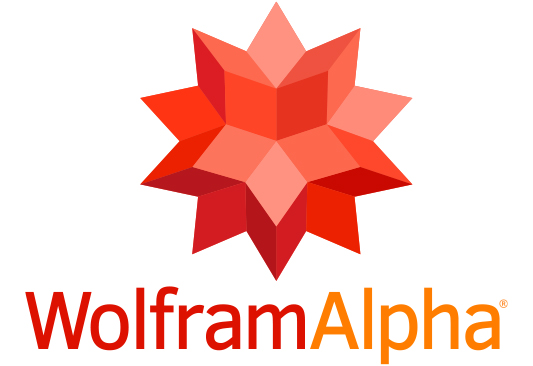
\includegraphics[width=0.25\textwidth]{img/chapter02/logo_wolfram.jpg}
	\caption[Logotipo de WolframAlpha.]{Logotipo de WolframAlpha. \textit{Fuente: ~\cite{wolframMatemathica}}}
	\label{fig:logo-wolfram}  % Etiqueta para la figura
\end{figure}
En contraste con otros motores de búsqueda, en vez de ofrecer una lista de sitios web o documentos, proporciona respuestas precisas y exhaustivas basándose en los conceptos introducidos en su motor de búsqueda. Entre algunas de sus capacidades, este potente software permite tiene funciones propias para resolver y graficar series de Fourier ~\cite{wolfram2024}:
%\begin{itemize}
%	\item \texttt{FourierSeries[exp, t, n]}: Calcula la expansión de la serie de Fourier de la función \texttt{exp} donde esta puede ser de un solo trozo o definida a varios trozos en términos de de la variable \texttt{t} hasta el \texttt{n}.
%	\item \texttt{FourierTrigSeries[exp, t, n]}: Expande en una serie trigonométrica...
%\end{itemize}
\begin{itemize}
		\item \texttt{FourierSeries[exp, t, n]}
		\item \texttt{FourierTrigSeries[exp, t, n]}
		\item \texttt{FourierSinSeries[exp, t, n]}
		\item \texttt{FourierCosSeries[exp, t, n]}
\end{itemize} 
Estas funciones nos permiten obtener expansión de la serie de Fourier, ya sea compleja, trigonométrica, en senos o cosenos  de una función \texttt{exp} con periodo de $2\pi$ donde esta puede ser de un solo trozo o definida a varios trozos, para esto se usaría la función \texttt{Piecewise[{{val1,cond1},{val2,cond2},…}]}~\cite{wolframMatemathicaPiecewise}, en términos de de la variable \texttt{t} hasta el \texttt{n}-ésimo término. Además nos mostrará una gráfica estática de una aproximación con \texttt{n} términos. También tiene funciones para calcular los coeficientes de la serie ~\cite{wolframMatemathica}:
\begin{itemize}
	\item \texttt{FourierSeriesCoefficient[exp, t, n]}
	\item \texttt{FourierSinCoefficient[exp, t, n]}
	\item \texttt{FourierCosCoefficient[exp, t, n]}
\end{itemize} 
Estas funciones nos permiten calcular el \texttt{n}-ésimo coeficiente de la serie de Fourier exponencial compleja, de senos o de cosenos, de una función \texttt{exp} con periodo de $2\pi$, recordando que puede ser a trozos o de un solo trozo. \newline
Podemos observar que las funciones propias de Wolfram Alpha para problemas que impliquen series de Fourier limitan el periodo en el que las funciones matemáticas son definidas, limitándolo en $2\pi$, para estos casos se podría resolver el coeficiente directamente usando la función de \texttt{Integrate[f,{x,xmin,xmax}]}~\cite{wolframMatemathicaPiecewise} para calcular individualmente cada coeficiente, ya sea $a_0, a_n$ y $b_n$ para las series trigonométricas o $c_0$ y $c_n$ para la serie compleja, pero así no nos proporciona la pequeña gráfica que si nos da al usar las funciones para expandir la serie, además de que la gráfica que se proporciona no es interactiva, y si quieremos verla con más detalle debemos pagar su suscripción.

\subsubsection{Prueba Wolfram Alpha}
Para nuestra primer prueba, calcularemos la serie de Fourier trigonométrica de la función calculada en el  \hyperref[app1:trig-coeff]{Apendice A}, para hacerlo usaremos la función \texttt{FourierTrigSeries(exp, t, n)} de WolframAlpha, que nos permite calcular la serie trigonométrica de Fourier de la función \texttt{exp} respecto a la variable \texttt{t} obteniendo la serie hasta el término \texttt{n}.
\begin{figure}[H]
	\centering
	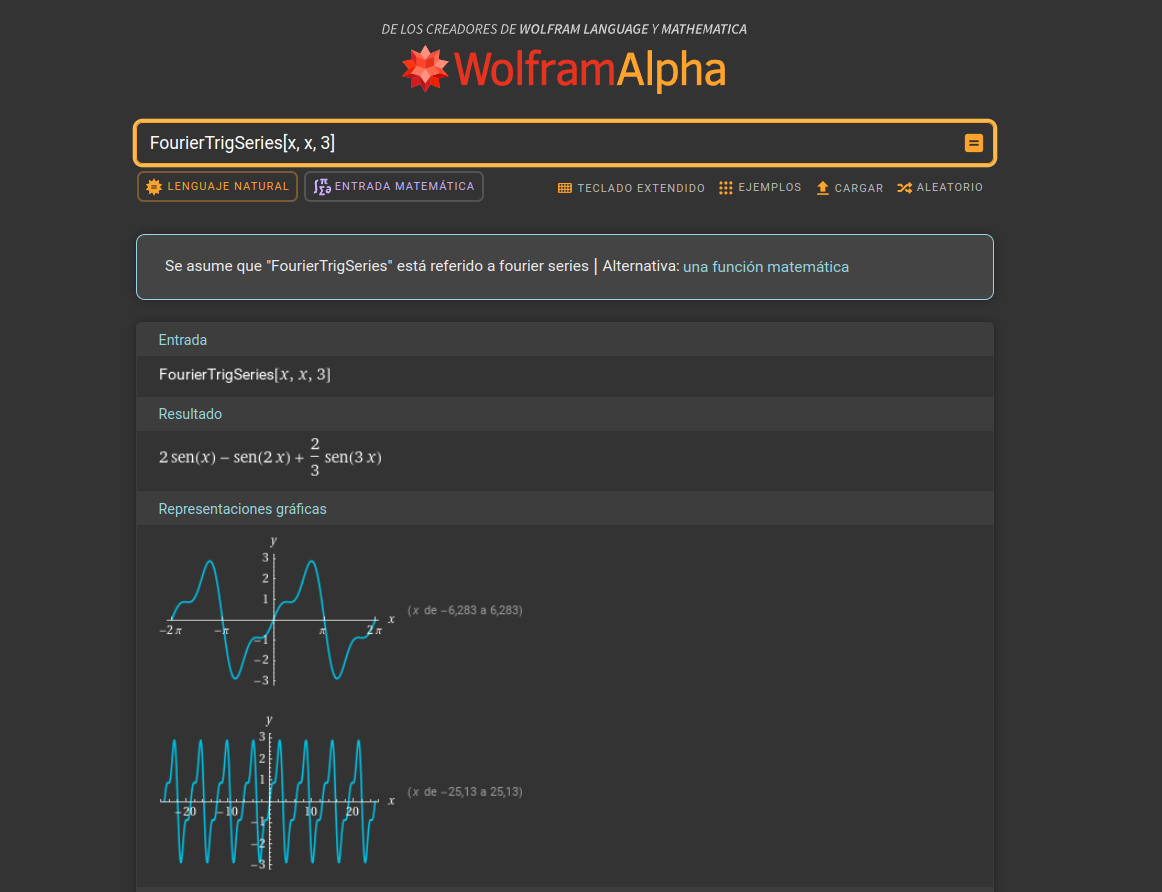
\includegraphics[width=1\textwidth]{img/chapter02/wolfram_trig_series.png}
	\caption{Calculo de una serie trigonométrica de Fourier en WolframAlpha}
	\label{fig:wolfram-trig-series}  % Etiqueta para la figura
\end{figure}
Ahora usaremos la función de \texttt{FourierSeries(exp, t, n)} de WolframAlpha, esta función no permite calcular la serie exponencial compleja de Fourier de la función \texttt{exp} respecto a la variable \texttt{t} obteniendo la serie hasta el término \texttt{n}.
\begin{figure}[H]
	\centering
	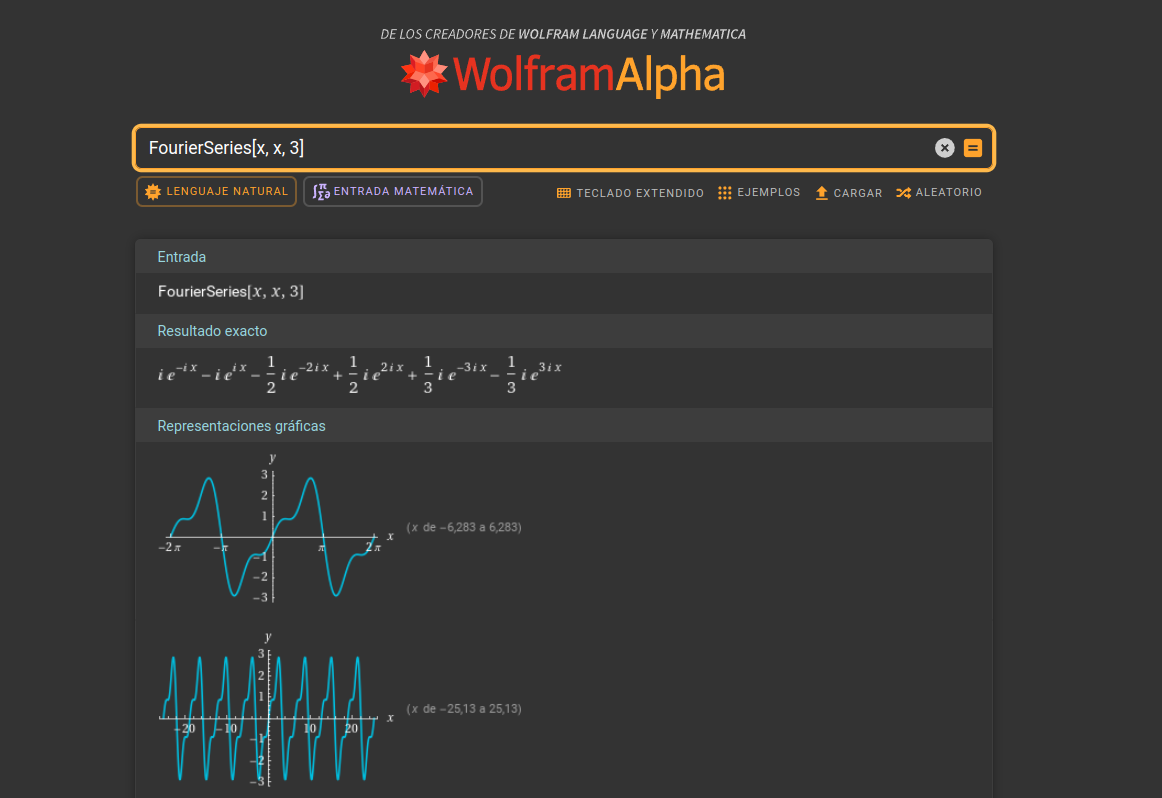
\includegraphics[width=1\textwidth]{img/chapter02/wolfram_complex_series.png}
	\caption{Calculo de una serie trigonométrica de Fourier en WolframAlpha}
	\label{fig:wolfram-exp-series}  % Etiqueta para la figura
\end{figure}
Wolfram nos devuelve la expansión de cada serie en su forma mas reducida, ademas de dos pequeñas gráficas de nuestra aproximación vista desde  no nos devuelve los coeficientes de la serie ni tampoco su expresión final en notación de serie.

\subsection{Symbolab}
Symbolab es una calculadora digital que ayuda a resolver problemas matemáticos, como ecuaciones, álgebra o cálculo. Se trata de una herramienta que cuyo principal proposito es ayudar a sus usuarios a aprender matemáticas, ya que ofrece resoluciones paso a paso y conocimientos impulsados por inteligencia artificial. ~\cite{symbolabDocs}. 
\begin{figure}[H]
	\centering
	
\includegraphics[width=0.15\textwidth]{img/chapter02/logo_symbolab.png}
	\caption[Logotipo de Symbolab.]{Logotipo de Symbolab. \textit{Fuente: ~\cite{symbolabDocs}}}
	\label{fig:logo-symbolab}  % Etiqueta para la figura
\end{figure}
Symbolab se centra en la enseñanza de procedimientos matemáticos mediante explicaciones detalladas. Su interfaz es especialmente útil para estudiantes, ya que presenta guías paso a paso para temas como derivadas, integrales y ecuaciones algebraicas complejas, lo cual es ideal para el aprendizaje autodidacta. Este cuenta con una función para resolver series de Fourier en su forma trigonométrica denominada \texttt{fourier series (f), [-L, L]} ~\cite{symbolabDocs} en donde \texttt{f} es una función definida en el intervalo de \texttt{[-L, L]}. A pesar de contar con funciones para definir funciones matemáticas a trozos y funciones para hacer gráficas, no es posible unificarlas en la misma aplicación, ademas de no contar con funciones para otras series de Fourier como extensiones de medio rango o exponencial compleja, pero, al igual que en Wolfram Alpha, se pueden calcular individualmente los coeficientes con la función \texttt{integral from a to b of x}~\cite{symbolabDocs}.

\subsubsection{Prueba Symbolab}
Para nuestra siguiente prueba, calcularemos la serie de Fourier trigonométrica de de la función calculada en el \hyperref[app1:trig-coeff]{Apendice A}, para hacerlo usaremos la función \texttt{fourier series (f), [-L, L]} de Symbolab, que nos permite calcular la serie trigonométrica de Fourier de la función \texttt{f} respecto a la variable obteniendo desde el intervalo \texttt{-L} a \texttt{L}.
\begin{figure}[H]
	\centering
	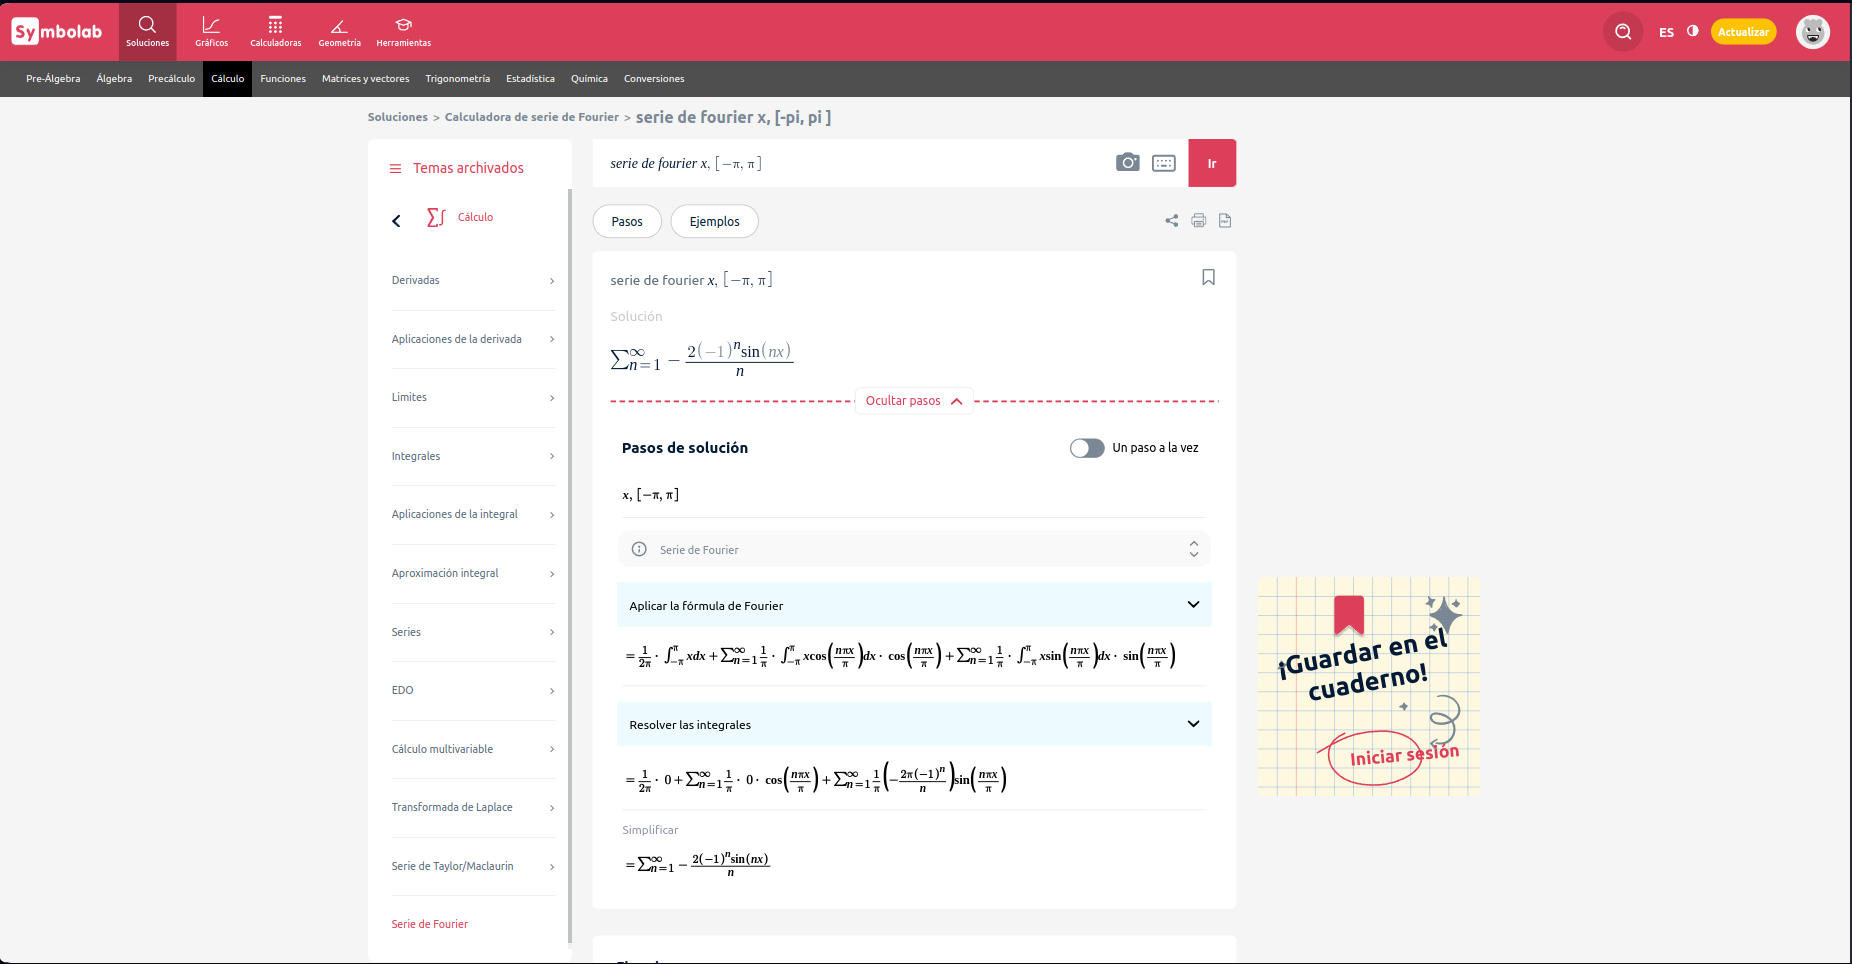
\includegraphics[width=1\textwidth]{img/chapter02/symbolab-trig-series.png}
	\caption{Calculo de una serie trigonométrica de Fourier en Symbolab}
	\label{fig:symbolab-trig-series}  % Etiqueta para la figura
\end{figure}
Symbolab nos dará la expresión en forma de serie, y solo podremos hacerlo para la serie trigonométrica, ademas de que no nos muestra ninguna gráfica.

\subsection{MATLAB} 
MATLAB es un entorno de programación y un lenguaje de alto nivel comercial ampliamente utilizado en ingeniería, física y matemáticas aplicadas para el análisis numérico, la visualización de datos y el desarrollo de algoritmos. Su robusta caja de herramientas, especialmente la \textit{Signal Processing Toolbox} y la \textit{Symbolic Math Toolbox}, facilitan el cálculo y la graficación de series de Fourier  ~\cite{MathWorks2024}.

\begin{figure}[H]
	\centering
	
\includegraphics[width=0.3\textwidth]{img/chapter02/logo_matlab.png}
	\caption[Logotipo de Matlab.]{Logotipo de Matlab. \textit{Fuente: ~\cite{MathWorks2024}}}
	\label{fig:logo-matlab}  % Etiqueta para la figura
\end{figure}

A pesar de que MATLAB cuenta con funciones especiales para el análisis de Fourier como la transformada de Fourier (\texttt{fourier(f)}) o la Transformada rápida de Fourier (\texttt{fft(f)}) no cuenta con funciones especificas para series de Fourier, sin embargo, podemos definir nuestros coeficientes para hacer el gráfico de ambas series.

\subsubsection{Prueba Matlab}
Para la prueba con Matlab, primero ejecutaremos el código en \hyperref[app2:trig-code-matlab]{Apendice B}, que nos graficará la serie de Fourier a partir de sus coeficientes trigonométricos \ref{fig:matlab-trig-series}. 
\begin{figure}[H]
	\centering
	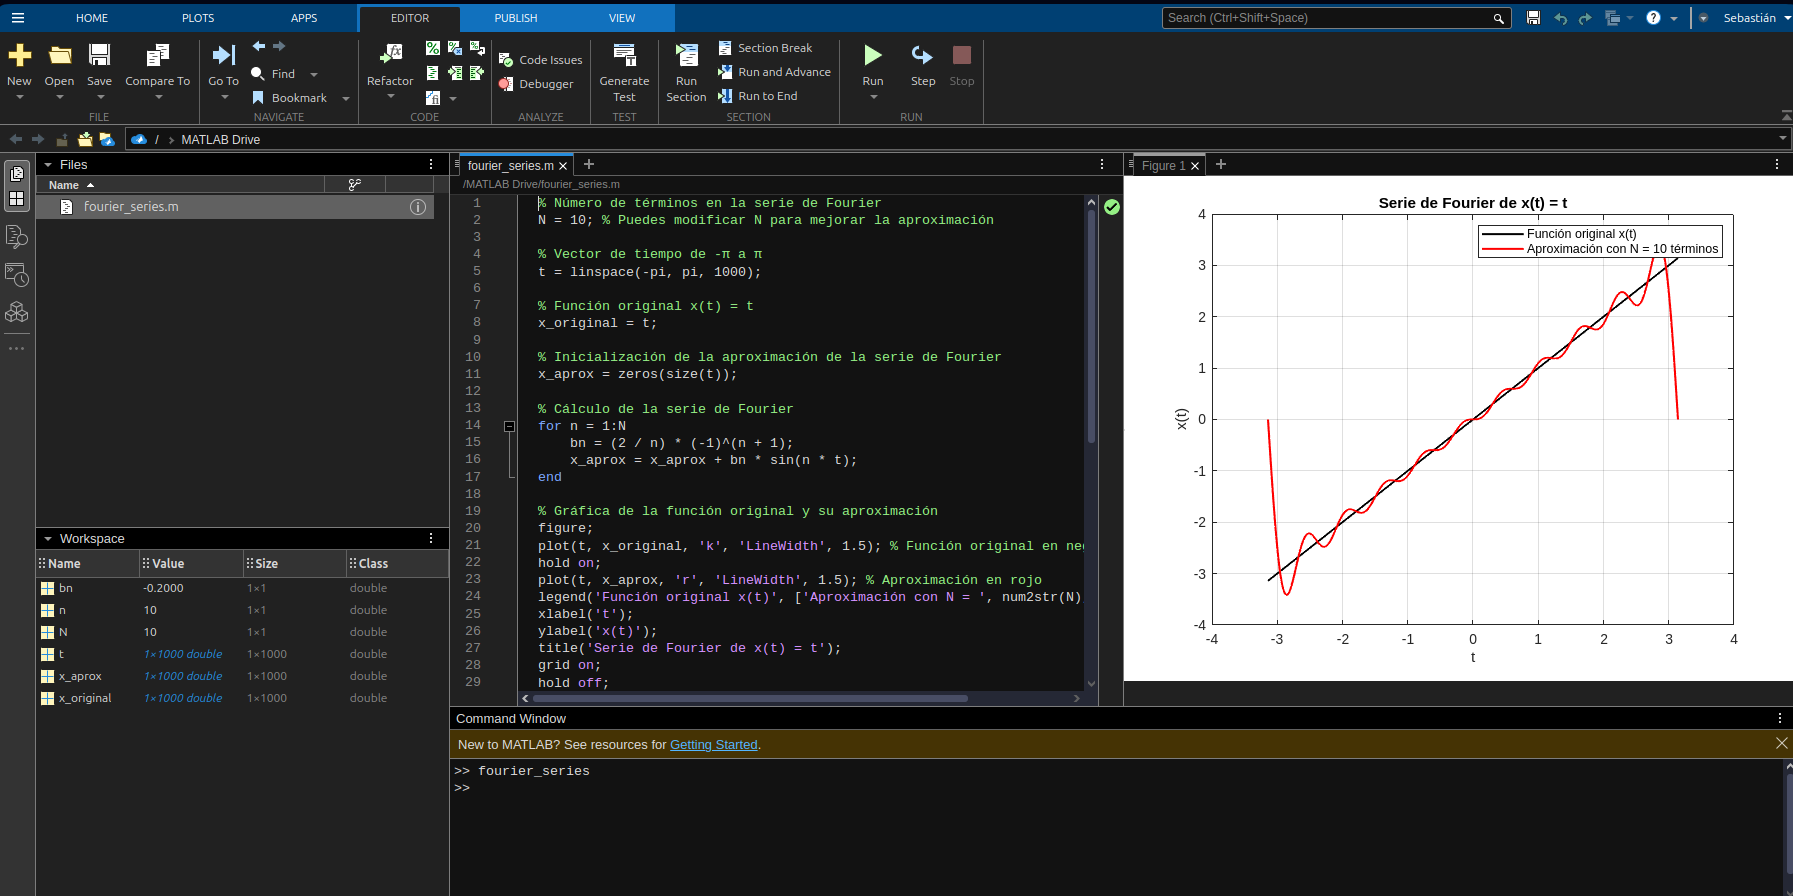
\includegraphics[width=1\textwidth]{img/chapter02/matlab-fourier-trig.png}
	\caption{Graficación de una serie trigonométrica de Fourier en Matlab}
	\label{fig:matlab-trig-series}  % Etiqueta para la figura
\end{figure}
Ahora usamos el código en \hyperref[app2:complex-code-matlab]{Apendice B} para graficar la misma serie pero ahora usando su coefciente complejo \ref{fig:matlab-complex-series}.
\begin{figure}[H]
	\centering
	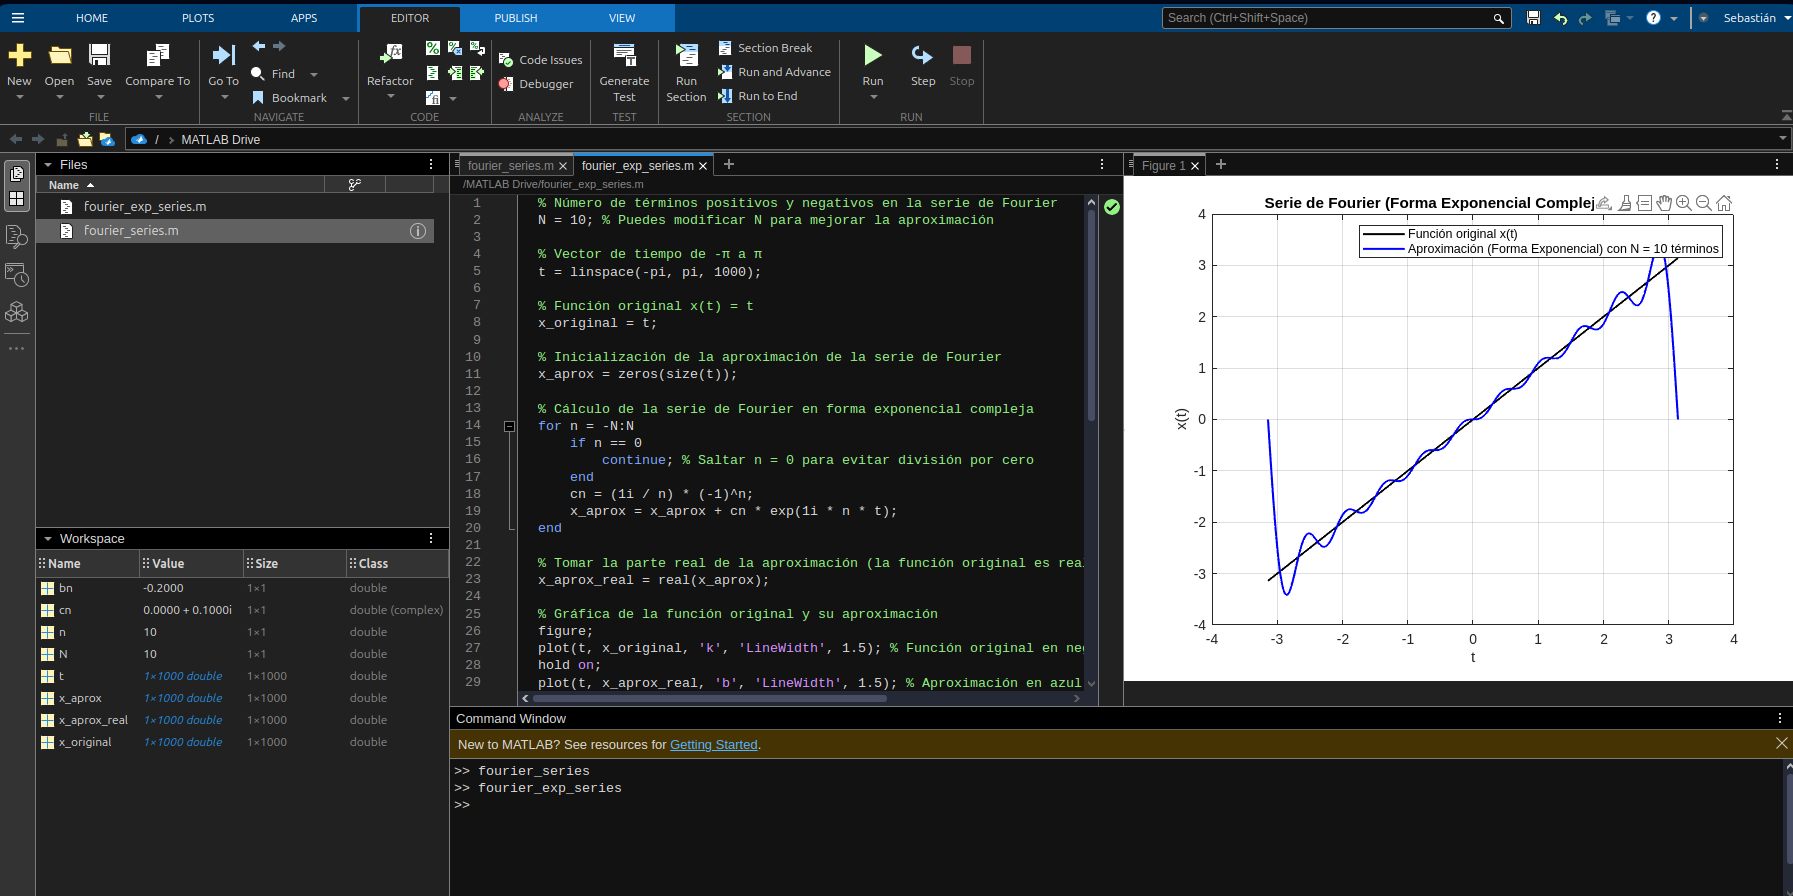
\includegraphics[width=1\textwidth]{img/chapter02/matlab-complex-series.png}
	\caption{Graficación de una serie compleja de Fourier en Matlab}
	\label{fig:matlab-complex-series}  % Etiqueta para la figura
\end{figure}
Matlab es capaz de graficar muy buenas aproximaciones de ambas series en una gráfica que nos brinda cierto nivel de interactividad pero todo dependerá de nuestros cálculos y de que tanto detalle plasmemos en nuestro código para aumentar las funcionalidades

\subsection{Maple}
Maple, desarrollado por Maplesoft, es un Sistema de Álgebra Computacional comercial que permite realizar cálculos matemáticos simbólicos y numéricos, resolver ecuaciones, analizar datos y crear visualizaciones gráficas en 2D y 3D. Maple utiliza el paradigma REPL (Read-Eval-Print Loop), un entorno interactivo donde cada línea de código ingresada es leída, evaluada y su resultado es impreso inmediatamente, facilitando así la experimentación y el desarrollo incremental de cálculos complejos.~\cite{maple2024}.
\begin{figure}[H]
	\centering
	
\includegraphics[width=0.3\textwidth]{img/chapter02/logo_maple.png}
	\caption[Logotipo de Maple.]{Logotipo de Maple. \textit{Fuente: ~\cite{maple2024}}}
	\label{fig:logo-maple}  % Etiqueta para la figura
\end{figure}
Si bien este CAS cuenta con funciones dedicadas al calculo de series de Fourier, estás vienen definidas en paquetes desarrollados por la comunidad de Maplesoft ~\cite{mapleFourier}, así que resulta más eficiente y conveniente usar las funciones de integración (\texttt{int(f, x = a..b)} calcula simbólicamente la integral de \texttt{f}, que depende de la variable \texttt{x} desde el punto \texttt{a} hasta el \texttt{b}) para calcular los coeficientes, y para expandir series (\texttt{seq(m, n = a..b)} en donde \texttt{m} es la función a sumar,sobre la variable \texttt{n} desde el punto \texttt{a} hasta el \texttt{b}) las funciones de expansión, además de poder declarar una función a trozos con la función \texttt{piecewise(cond-1, f-1, cond-2, f-2, ..., cond-n, f-n, f-otherwise)}.

\subsubsection{Prueba Maple}
Para la prueba con Maple, primero ejecutaremos el código en \hyperref[app2:trig-code-maple]{Apendice B}, que, primeramente, calculará los coeficientes de la serie trigonométrica \ref{fig:maple-trig-series}. 
\begin{figure}[H]
	\centering
	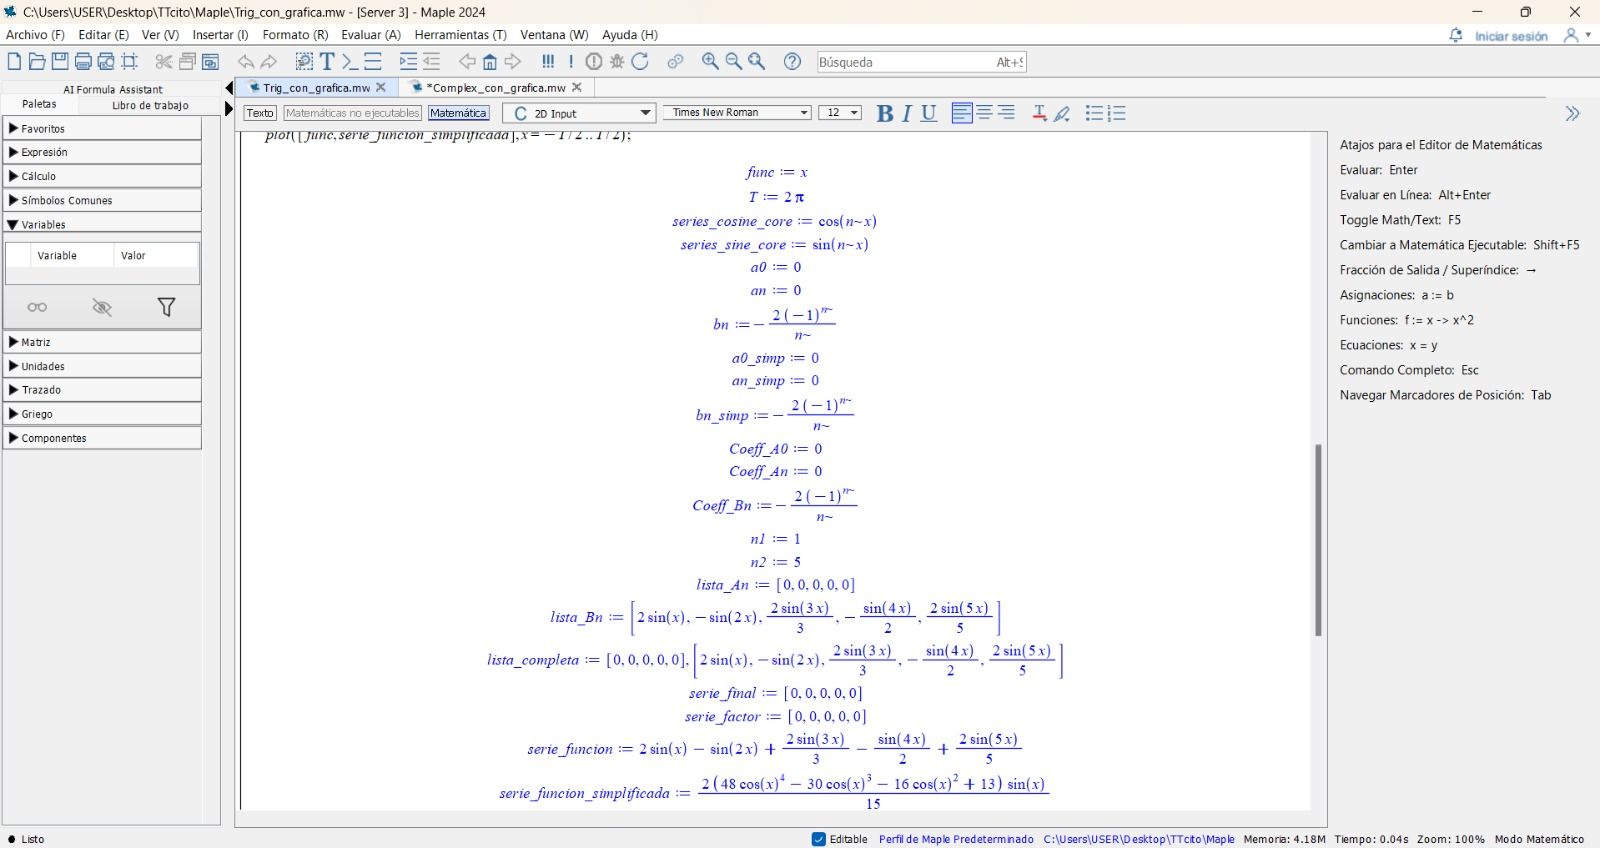
\includegraphics[width=1\textwidth]{img/chapter02/maple-trig-series-coeff.jpeg}
	\caption{Cálculos de coeficientes trigonométricos de Fourier en Maple}
	\label{fig:maple-trig-series}  % Etiqueta para la figura
\end{figure}

Posteriormente, este código nos dará una gráfica estática con los valores que le establecimos \hyperref[app2:trig-code-maple]{Apendice B} \ref{fig:maple-trig-series-graph}. 
\begin{figure}[H]
	\centering
	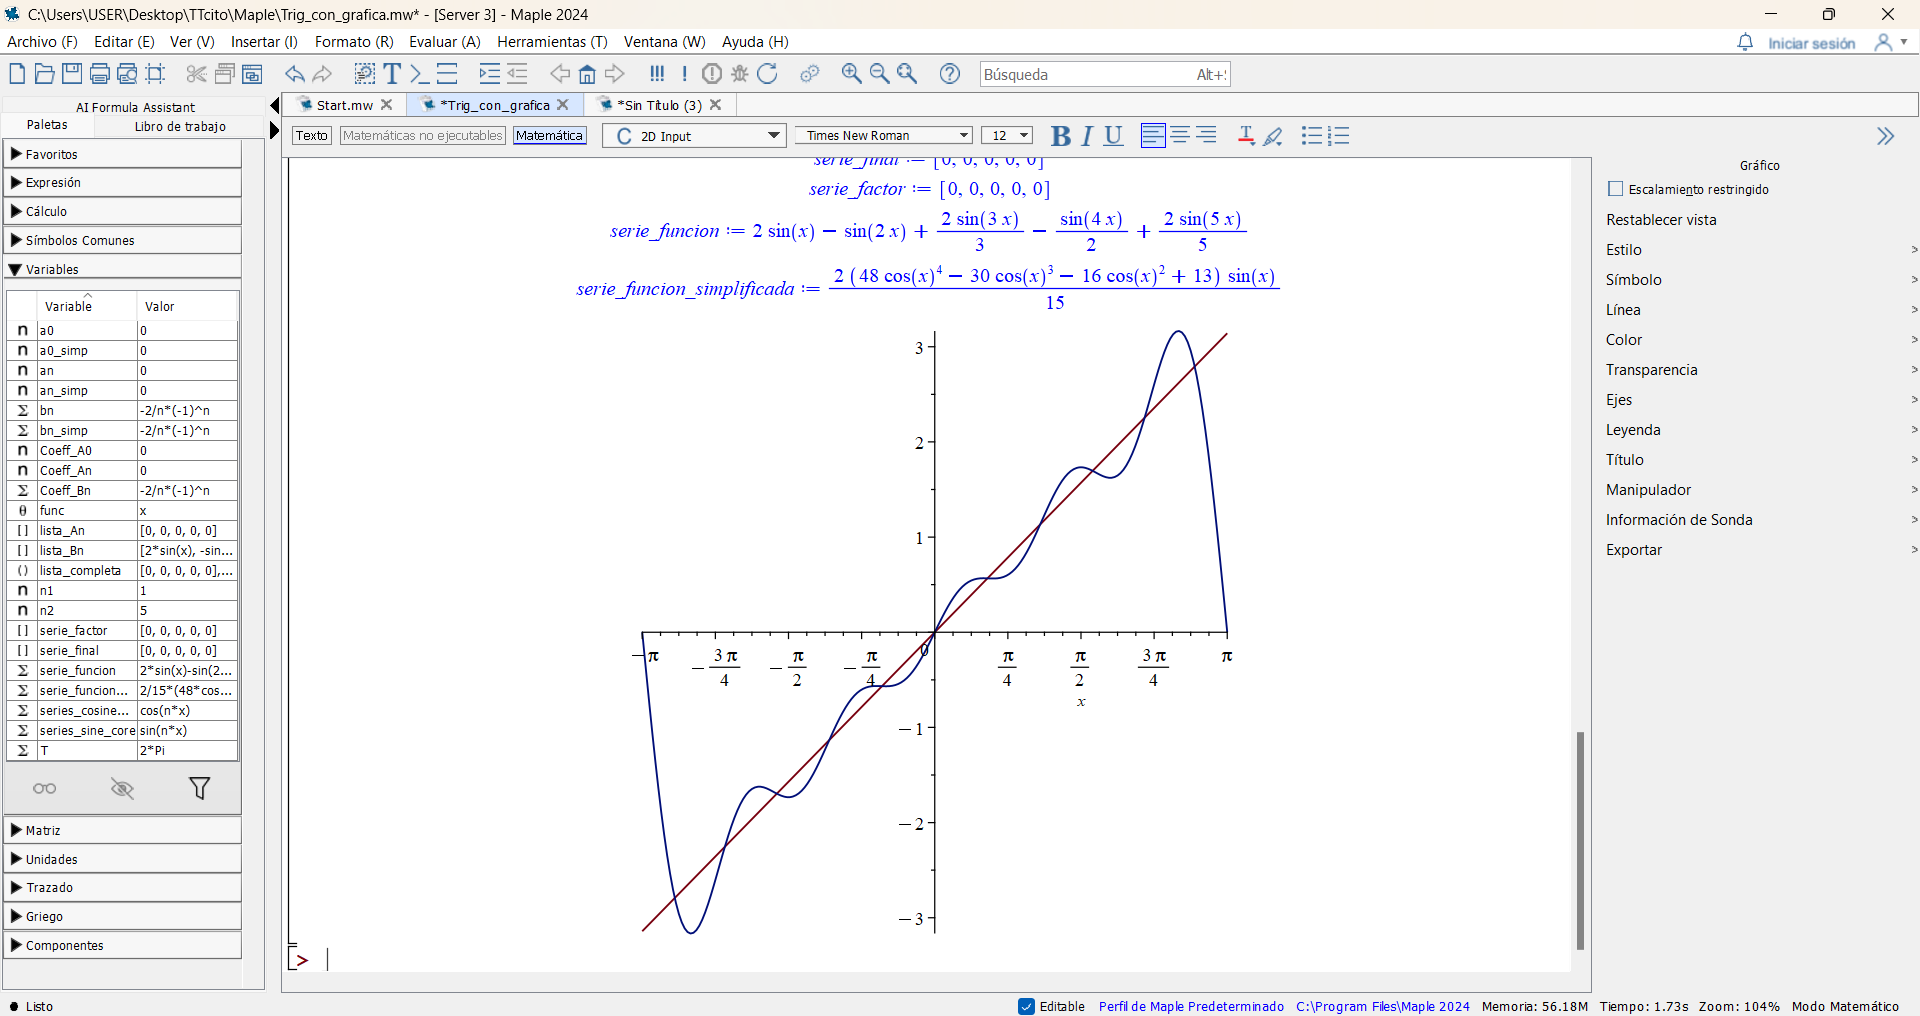
\includegraphics[width=1\textwidth]{img/chapter02/maple-trig-graph.png}
	\caption{Grafica de la serie de Fourier trigonométrica en Maple}
	\label{fig:maple-trig-series-graph}  % Etiqueta para la figura
\end{figure}
Podemos ver que puede resolver la serie trigonométrica sin problema alguno, ahora veamos la misma función pero desarrollada en una serie exponencial compleja  \hyperref[app2:complex-code-maple]{Apendice B}.
\begin{figure}[H]
	\centering
	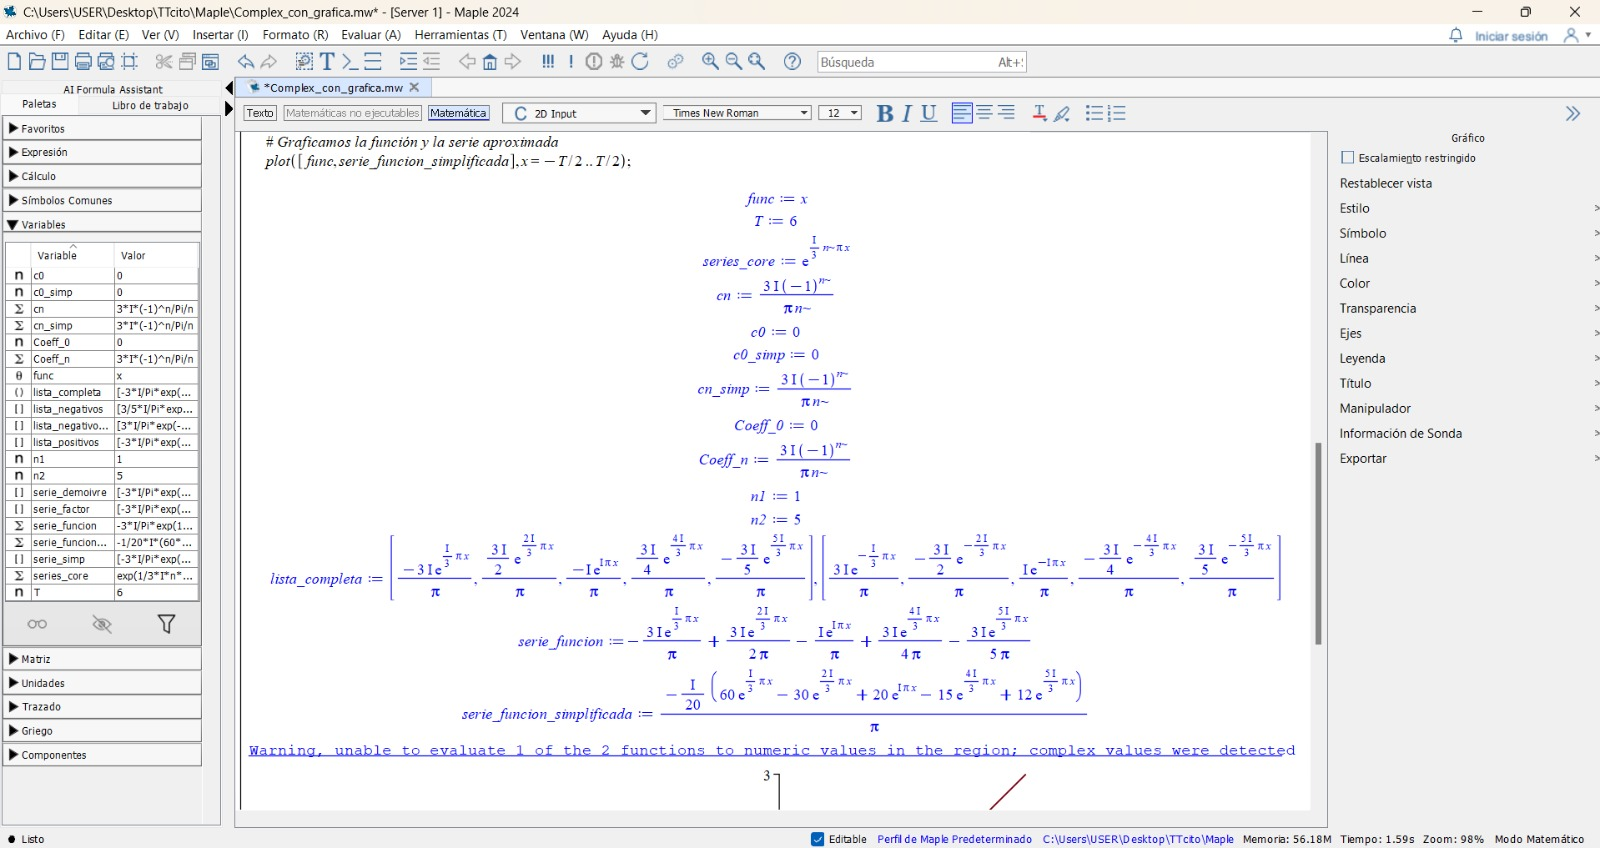
\includegraphics[width=1\textwidth]{img/chapter02/maple-complex-series-coeff.jpeg}
	\caption{Cálculo del coeficiente complejo de Fourier en Maple}
	\label{fig:maple-complex-series}  % Etiqueta para la figura
\end{figure}

De igual modo, este código nos dará una gráfica estática con los valores que le establecimos \hyperref[app2:trig-code-maple]{Apendice B} \ref{fig:maple-trig-series-graph}. 
\begin{figure}[H]
	\centering
	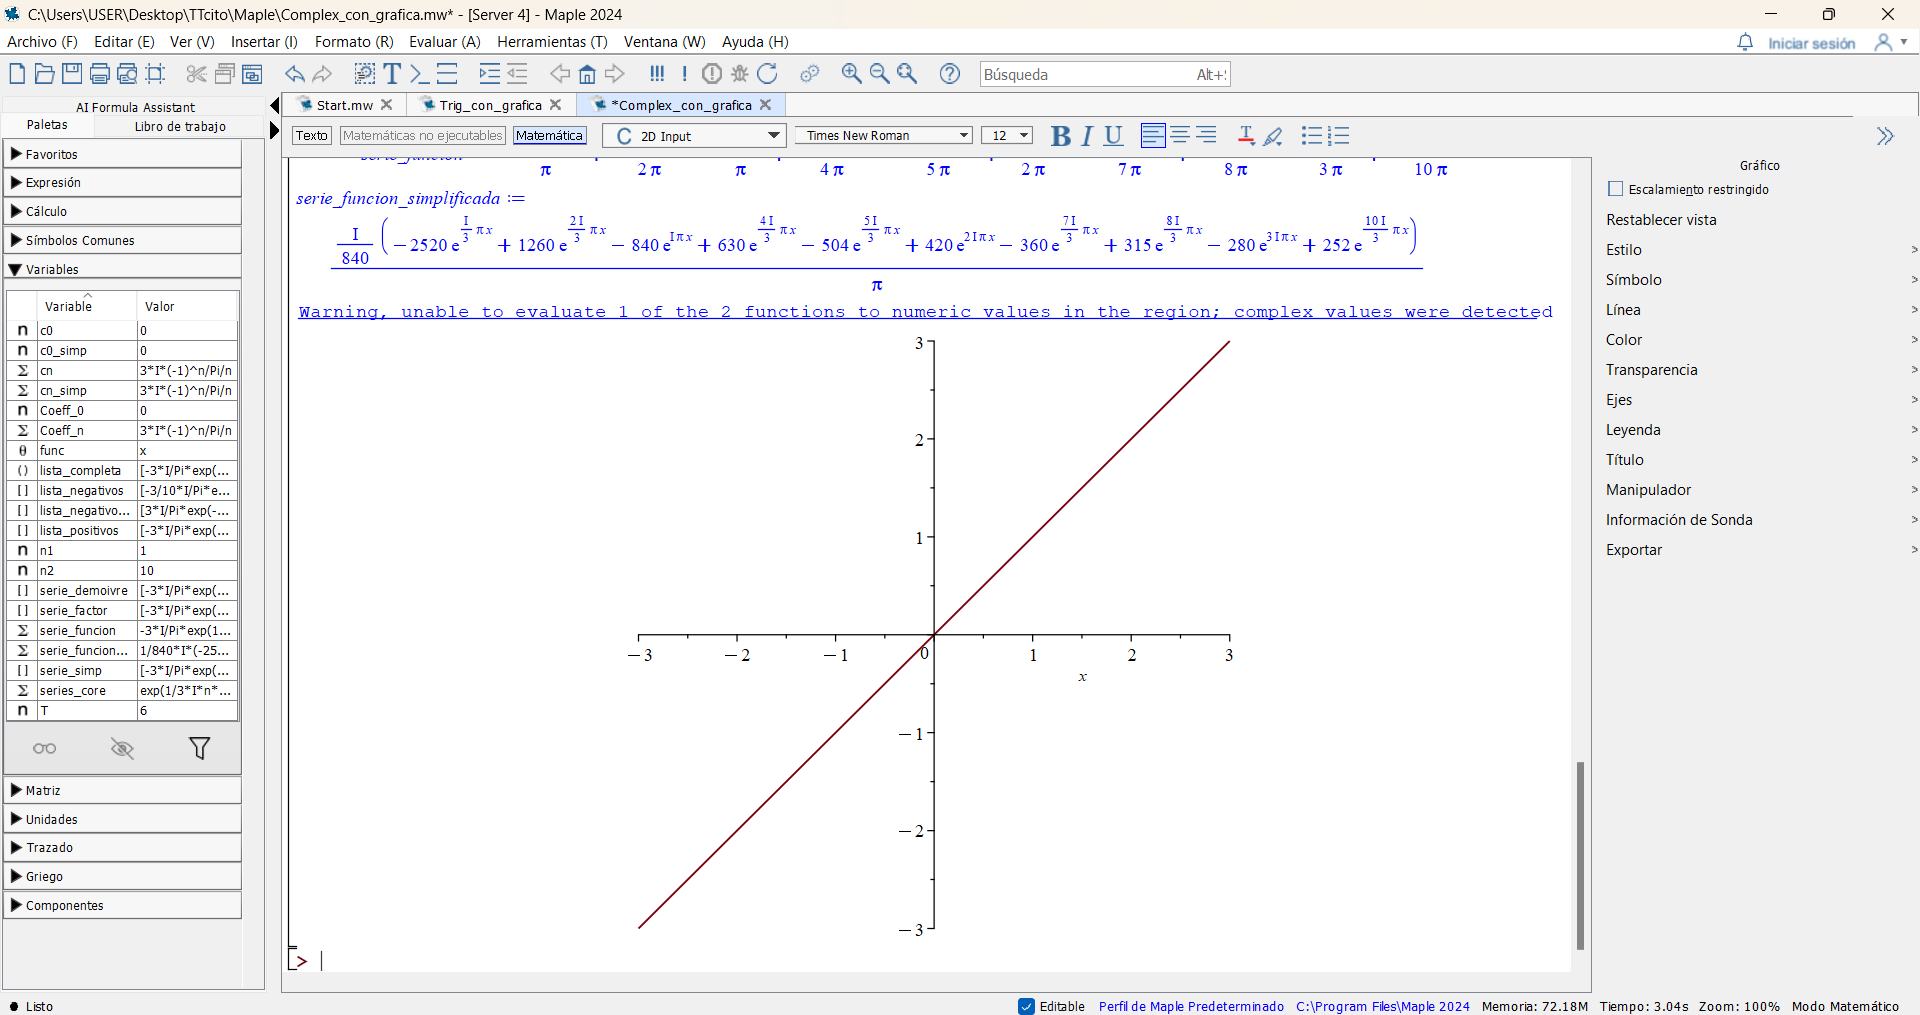
\includegraphics[width=1\textwidth]{img/chapter02/maple-complex-graph.png}
	\caption{Grafica de la serie de Fourier compleja en Maple}
	\label{fig:maple-complex-series-graph}  % Etiqueta para la figura
\end{figure}
El detalle está en que no hay forma de graficar nuestra función serie compleja ya que no puede hacer las cancelaciones entre los números imaginarios al expandir la serie, por lo tanto, la función la mantiene en el dominio de los números complejos y no la puede graficar en el plano real. Una alternativa sería graficar la serie trigonométrica que obtuvimos en \ref{fig:maple-trig-series-graph} ya que son equivalentes.

\subsection{Maxima}
Maxima es un Sistema de Álgebra Computacional de código abierto y gratuito, derivado del sistema Macsyma desarrollado en la década de 1980. Permite realizar cálculos simbólicos y numéricos avanzados, como derivadas, integrales, simplificación de expresiones algebraicas, resolución de ecuaciones y generación de gráficos en 2D y 3D. Maxima emplea el paradigma REPL (Read-Eval-Print Loop), proporcionando un entorno interactivo donde cada comando ingresado se procesa de inmediato, lo que facilita la verificación y corrección rápida de cálculos ~\cite{MaximaSourgeforce}. 
\begin{figure}[H]
	\centering
	
\includegraphics[width=0.25\textwidth]{img/chapter02/logo_maxima.png}
	\caption[Logotipo de Maxima.]{Logotipo de Maxima. \textit{Fuente: ~\cite{MaximaSourgeforce}}}
	\label{fig:logo-maxima}  % Etiqueta para la figura
\end{figure}
Si bien, este CAS al igual que Maple, cuenta con módulo que importa funciones especiales para el análisis de Fourier, este si es propio de Maxima. Sin embargo, igual que en Maple, resulta más practico trabajar con las funciones propias de Maxima para integrar (\texttt{integrate (expr, x, a, b)} Calcula simbólicamente la integral de \texttt{expr} con límites en \texttt{a} y \texttt{b} ) así como su función para expandir una función en serie (\texttt{makelist(expr, i, i\_min, i\_max, step)} Genera una lista evaluando \texttt{expr} para cada valor de \texttt{i} desde \texttt{i\_min} hasta \texttt{i\_max}, incrementando \texttt{i} en \texttt{step} en cada iteración). 

\subsubsection{Prueba Maxima}
Para la prueba con Maxima, ejecutaremos el código en \hyperref[app2:trig-code-maxima]{Apendice B}, que primero calculará los coeficientes de la serie trigonométrica \ref{fig:maple-trig-series}. 
\begin{figure}[H]
	\centering
	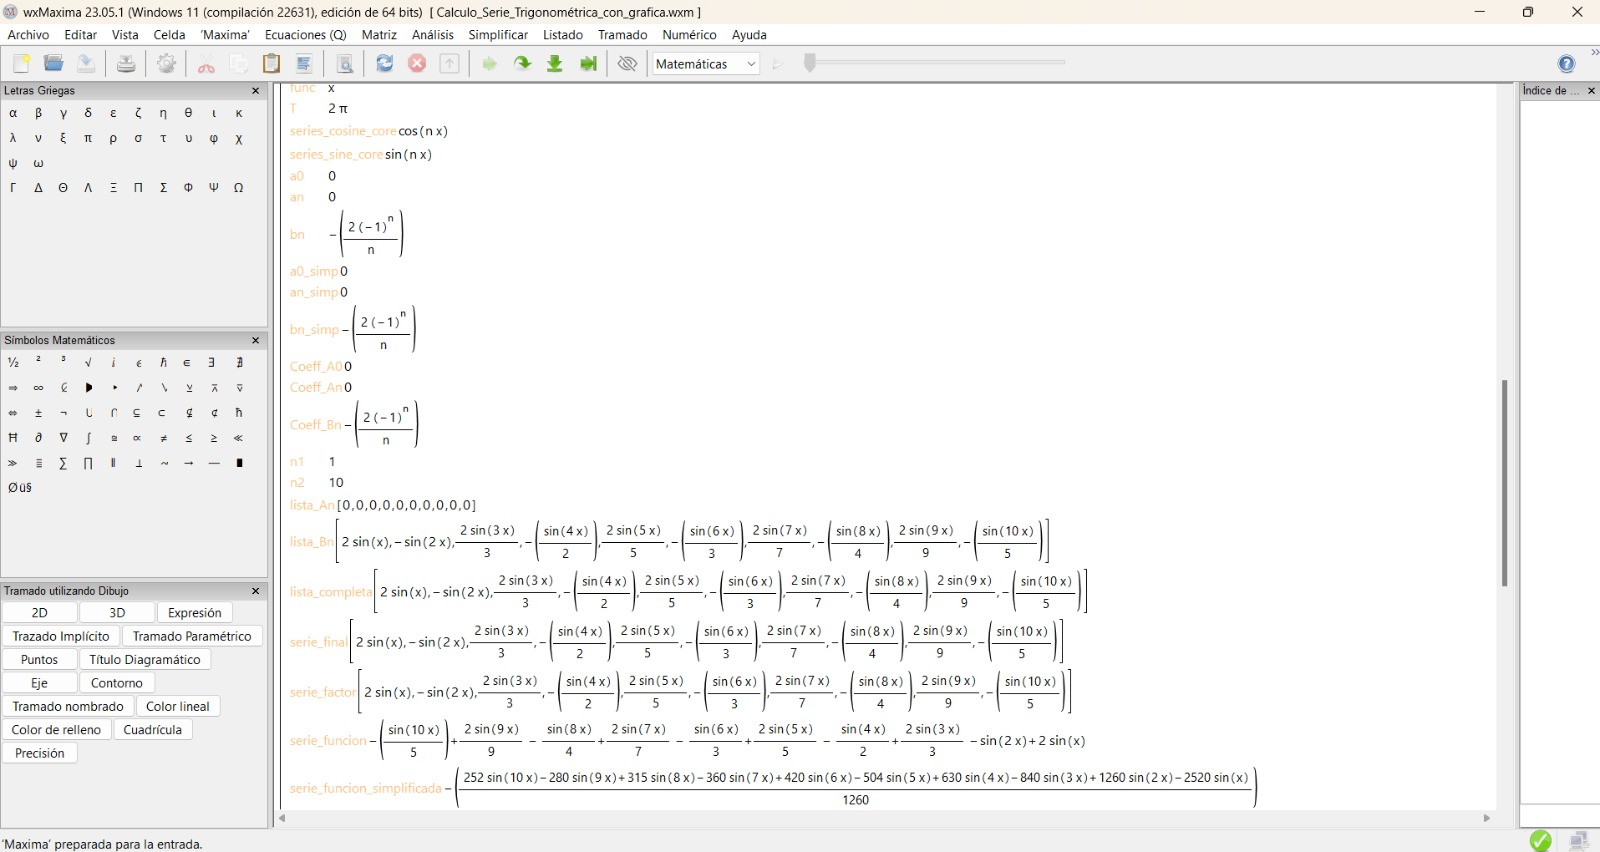
\includegraphics[width=1\textwidth]{img/chapter02/maxima-trig-series-coeff.jpeg}
	\caption{Cálculos de coeficientes trigonométricos de Fourier en Maxima}
	\label{fig:maxima-trig-series}  % Etiqueta para la figura
\end{figure}
Posteriormente, este código nos dará una gráfica dinámica con los valores que le establecimos.
\begin{figure}[H]
	\centering
	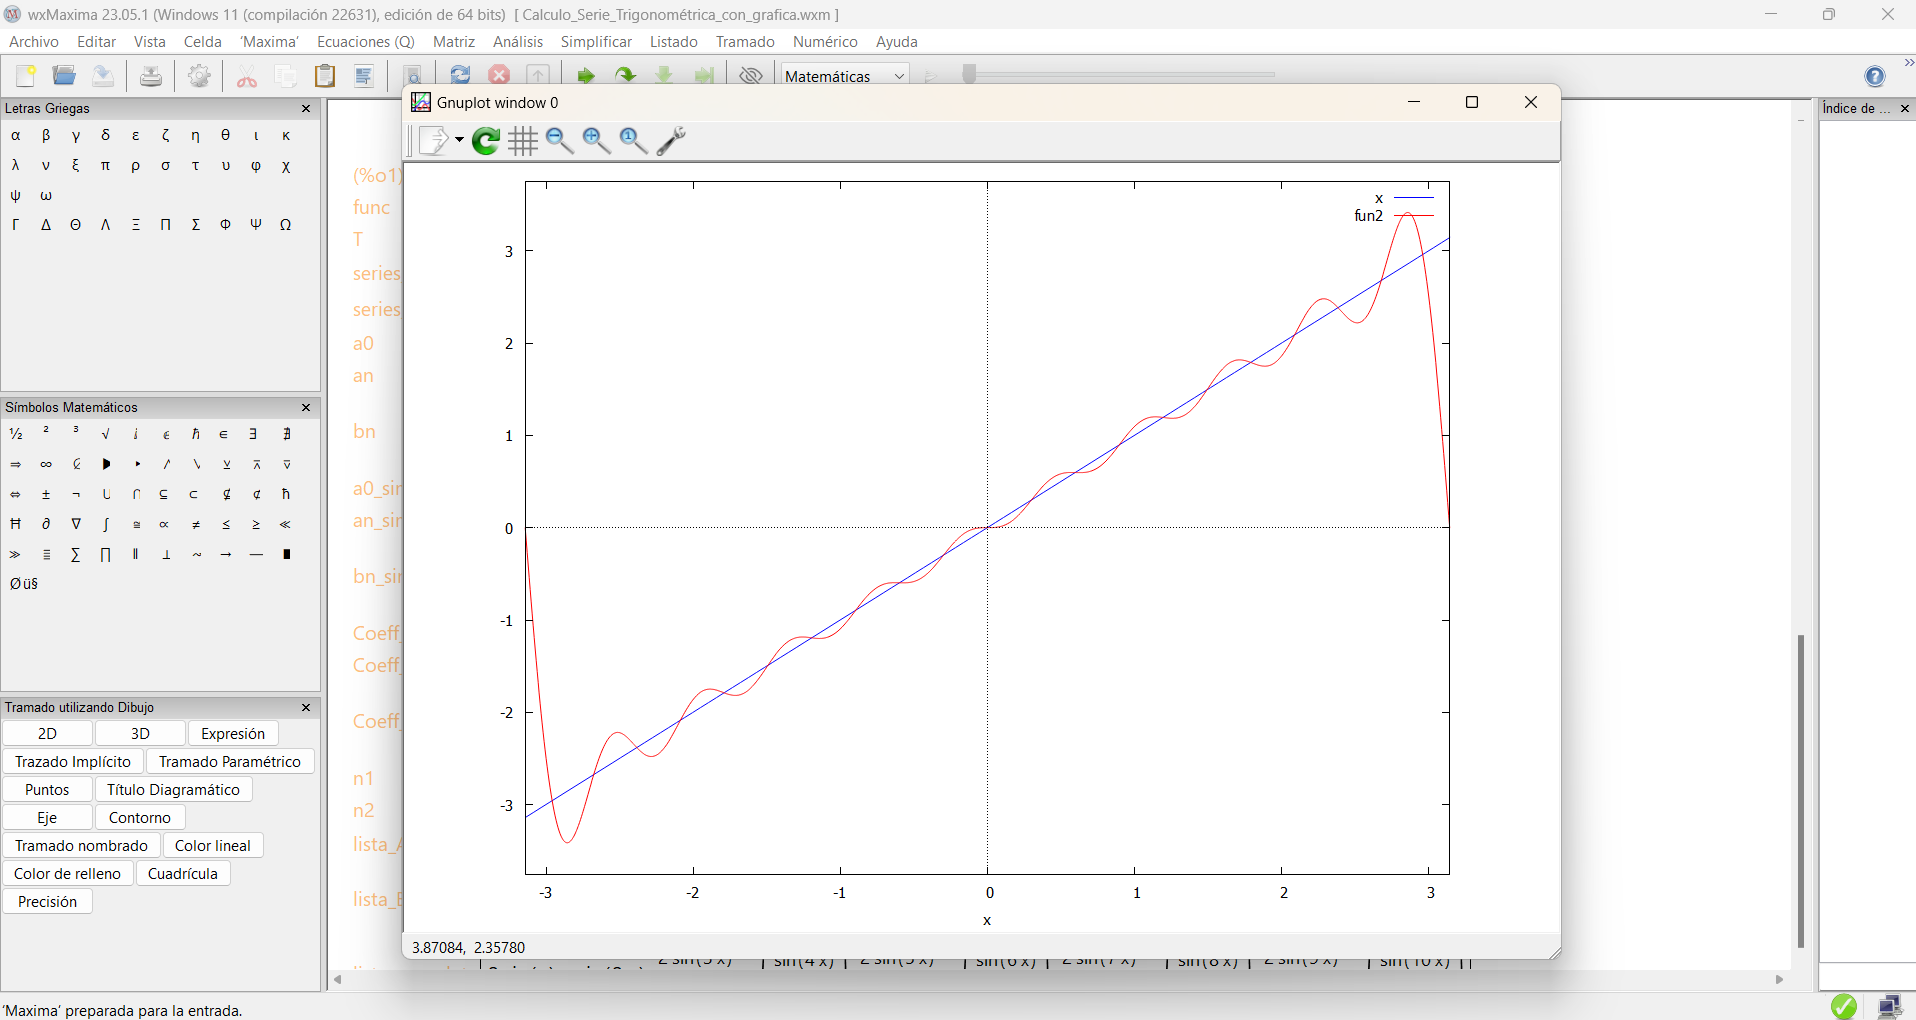
\includegraphics[width=1\textwidth]{img/chapter02/maxima-trig-series-graph.png}
	\caption{Grafica de la serie de Fourier trigonométrica en Maxima}
	\label{fig:maxima-trig-series-graph}  % Etiqueta para la figura
\end{figure}

Podemos ver que sin problema alguno se construye la gráfica, ahora, probemos haciendo el problema de la misma función pero para la serie compleja  \hyperref[app2:complex-code-maxima]{Apendice B}. 

\begin{figure}[H]
	\centering
	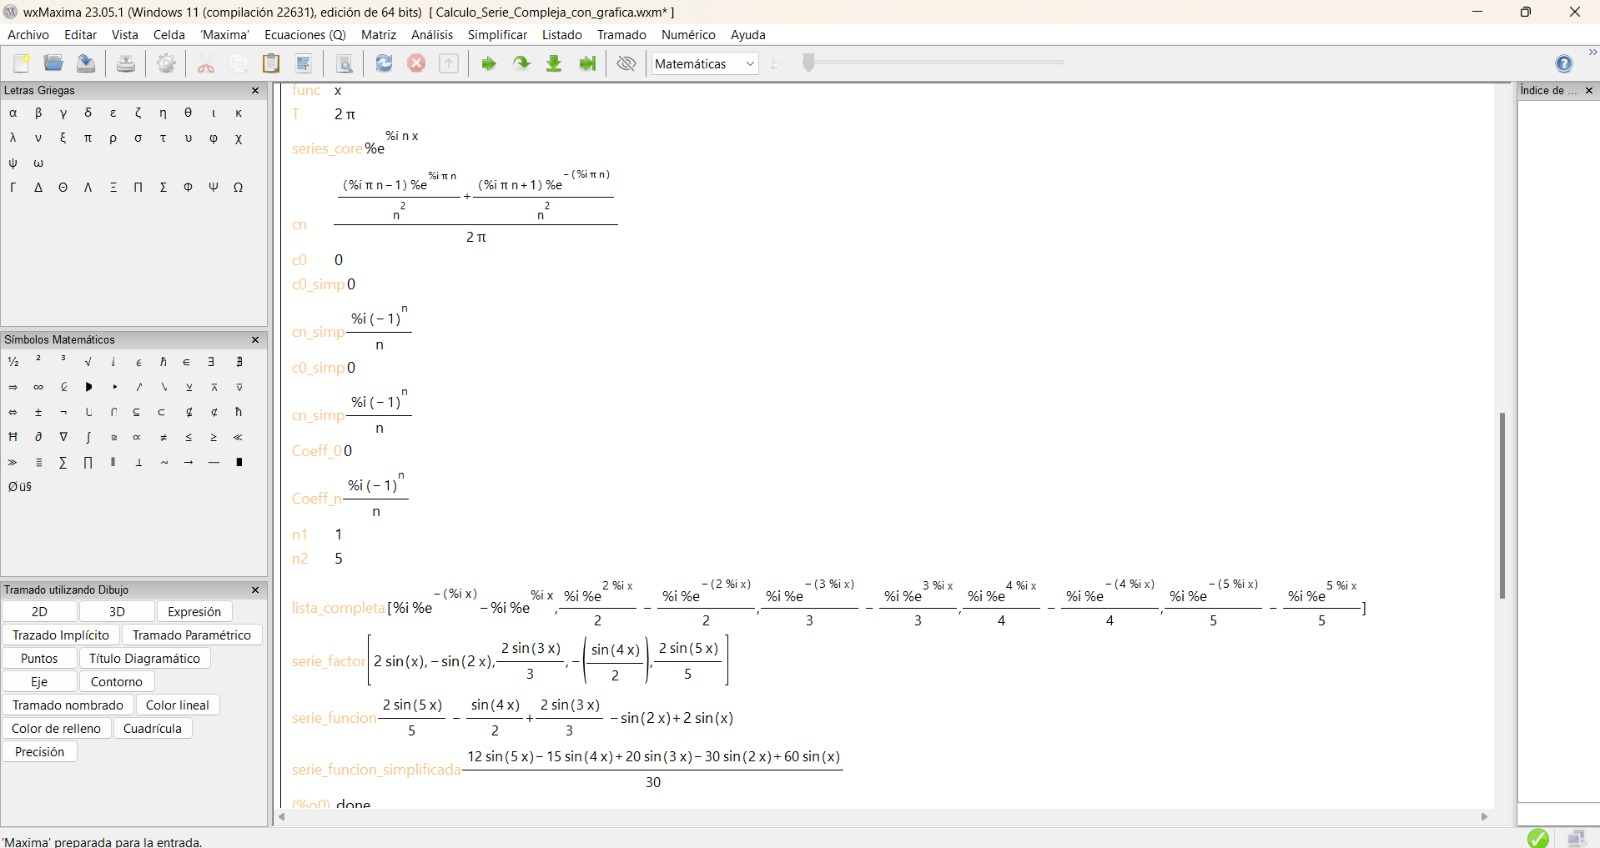
\includegraphics[width=1\textwidth]{img/chapter02/maxima-complex-series-coeff.jpeg}
	\caption{Cálculos de coeficientes compleja de Fourier en Maxima}
	\label{fig:maxima-complex-series}  % Etiqueta para la figura
\end{figure}
De igual modo, este código nos dará una gráfica dinámica con los valores que le establecimos.
\begin{figure}[H]
	\centering
	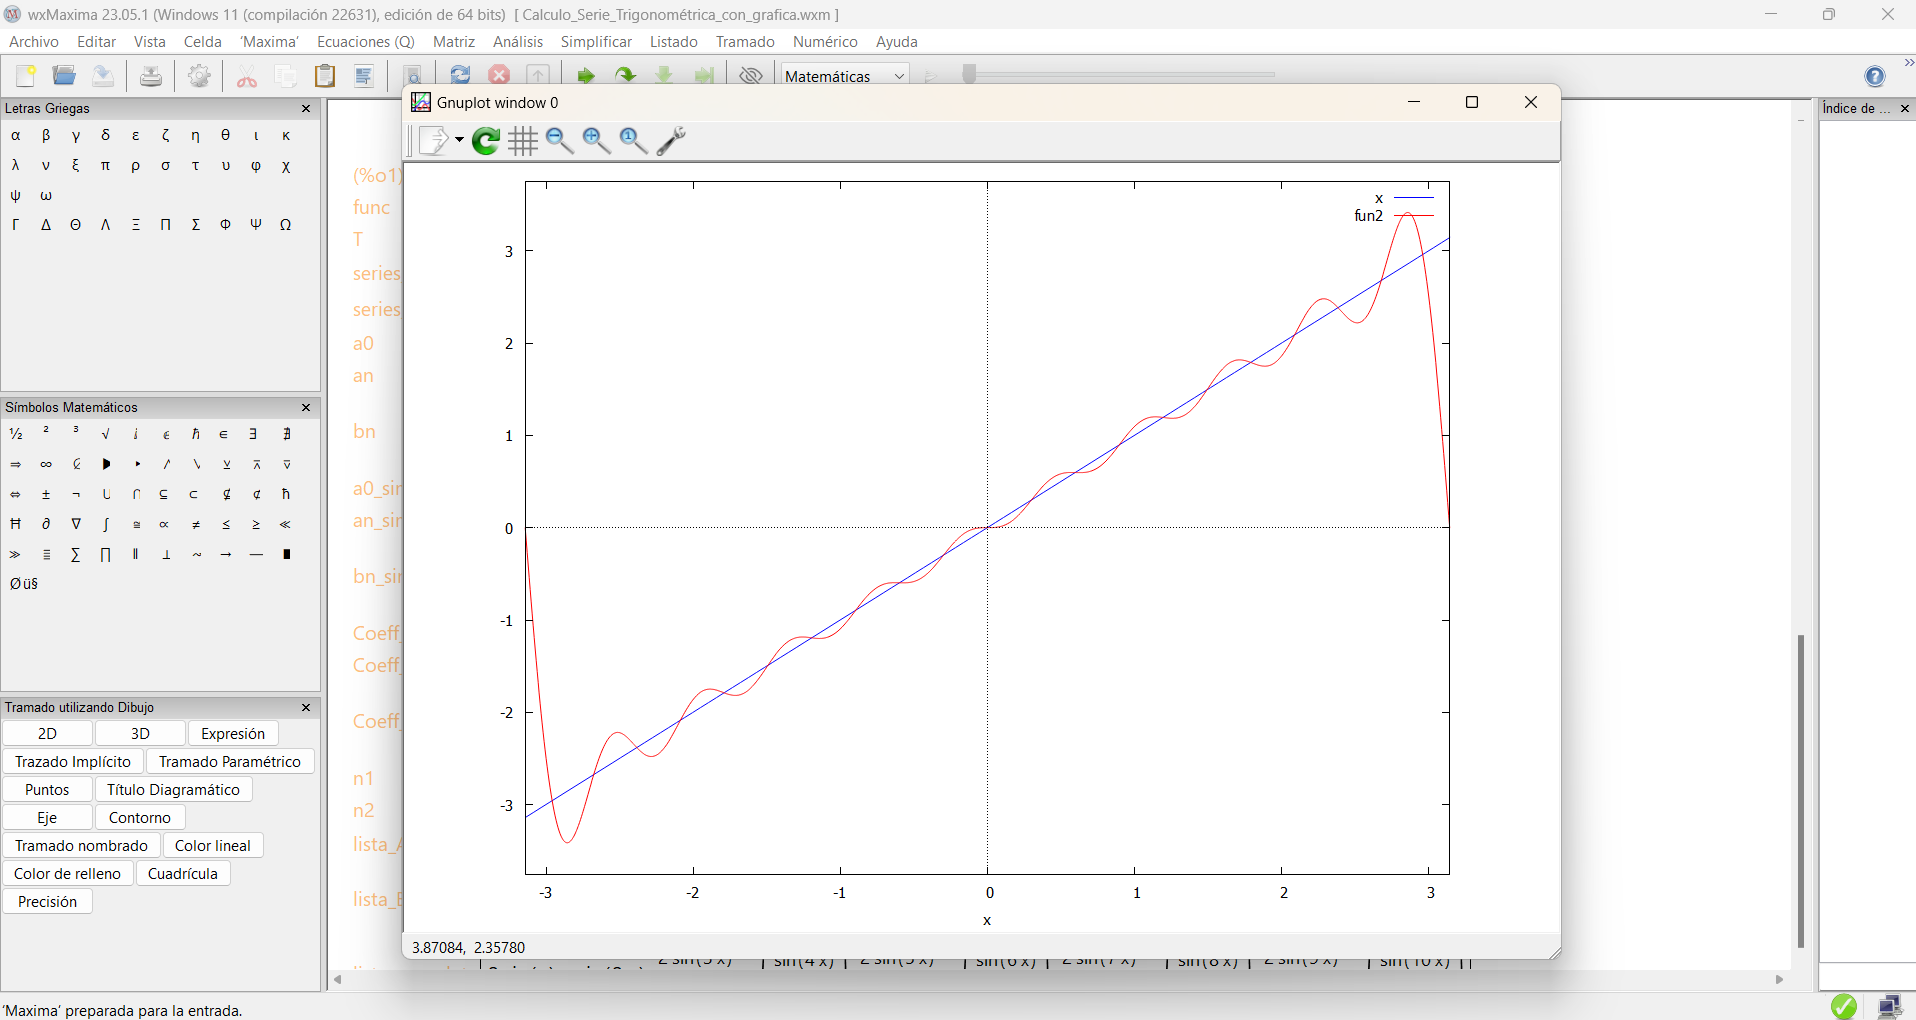
\includegraphics[width=1\textwidth]{img/chapter02/maxima-trig-series-graph.png}
	\caption{Grafica de la serie de Fourier compleja en Maxima}
	\label{fig:maxima-complex-series-graph}  % Etiqueta para la figura
\end{figure}
Podemos observar que sin problemas podemos hacer el gráfico ya que la función \texttt{demoivre()} se encarga de separar la parte real e imaginaria y con esto, hacer la gráfica equivalente.
A pesar de que Maxima no cuenta con una función para declarar funciones a trozos, podemos calcular las integrales por separado o usar matrices (\texttt{matrix (fila\_1, ..., fila\_n)}), pero esto se verá más adelante. 
\subsection{Geogebra / Desmos}
GeoGebra y Desmos son dos herramientas educativas digitales, gratuitas y de código abierto, utilizadas para la enseñanza y el aprendizaje de las matemáticas. Ambas permiten a los usuarios graficar funciones, trabajar conceptos algebraicos y geométricos de manera interactiva, facilitando la visualización y comprensión de diversos temas matemáticos. Estas presentan algunas diferencias: GeoGebra ofrece una suite más completa que incluye módulos para álgebra, geometría, cálculo y estadística, lo que la hace especialmente útil para crear construcciones geométricas dinámicas y realizar análisis más complejos ~\cite{GeoGebra2024}. Por otro lado, Desmos se destaca por su interfaz intuitiva y facilidad de uso, enfocándose principalmente en la gráfica de funciones y proporcionando herramientas sencillas para crear visualizaciones rápidas y efectivas, lo que la hace ideal para estudiantes y educadores que buscan una plataforma accesible y potente para la enseñanza de conceptos fundamentales ~\cite{Desmos2024}.

\begin{figure}[H]
	\centering
	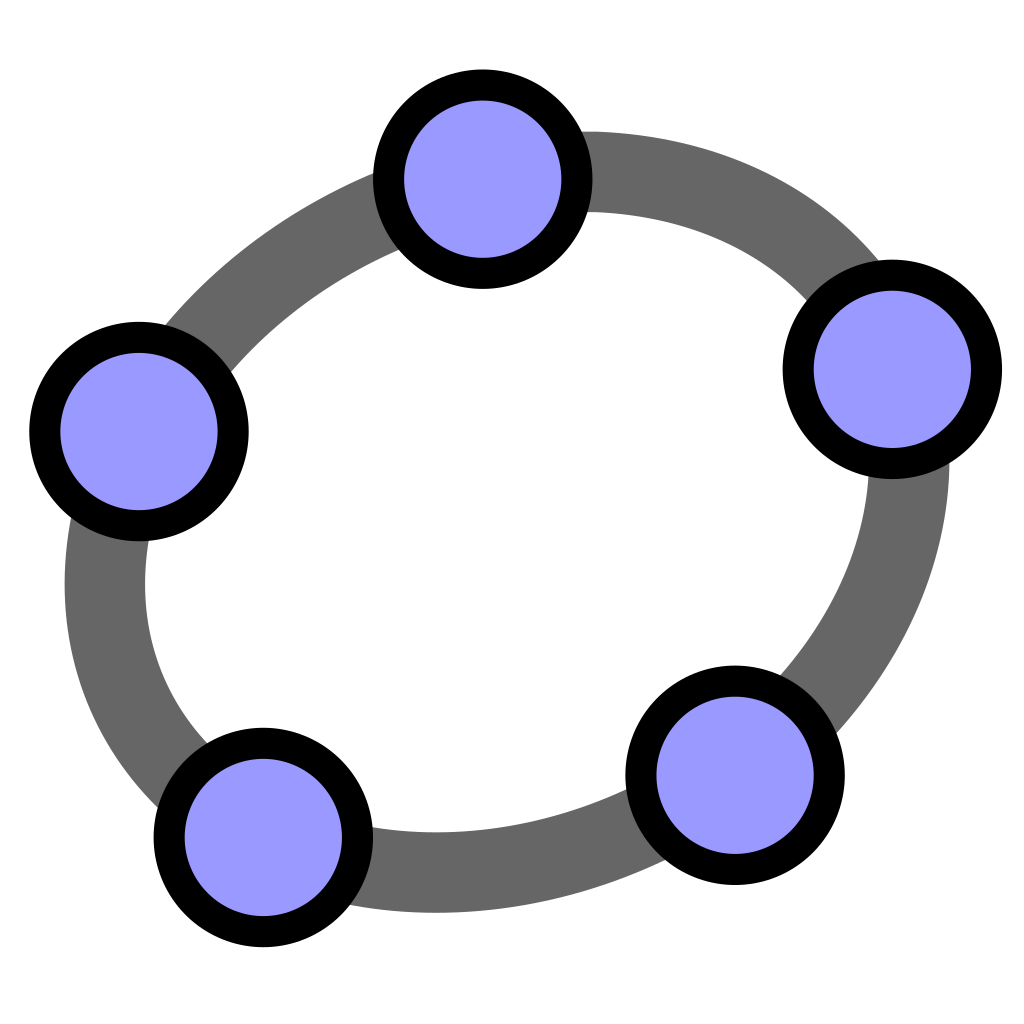
\includegraphics[width=0.2\textwidth]{img/chapter02/logo_geogebra.png}
	\caption[Logotipo de Geogebra.]{Logotipo de Geogebra. \textit{Fuente: ~\cite{GeoGebra2024}}}
	\label{fig:logo-geogebra}
\end{figure}


\begin{figure}[H]
	\centering
	
\includegraphics[width=0.3\textwidth]{img/chapter02/logo_desmos.jpg} 
	\caption[Logotipo de Desmos.]{Logotipo de Desmos. \textit{Fuente: ~\cite{Desmos2024}}}
	\label{fig:logo-desmos}
\end{figure}

Si bien, no tienen funciones especificas para el análisis de Fourier, ambas pueden hacer las gráficas de sumas correspondientes a los coeficientes. A continuación mostraremos la gráfica de la serie de Fourier de \ref{app1:trig-coeff} con ambas herramientas.

\subsubsection{Prueba Geogebra}
Para la prueba con Geogebra, crearemos un slider desde 1 hasta el valor que querramos con la única condición de que este de saltos de 1 en 1, es decir, sea un slider de números enteros, también usamos la función de \texttt{Suma(Expresión, Variable, Valor Inicial, Valor Final)} en donde \texttt{Expresión} será la función de la serie, \texttt{Variable} es el n-ésimo termino en la serie, \texttt{Valor Inicial} será 1 y   \texttt{Valor Final} será el valor que toma el slider.
\begin{figure}[H]
	\centering
	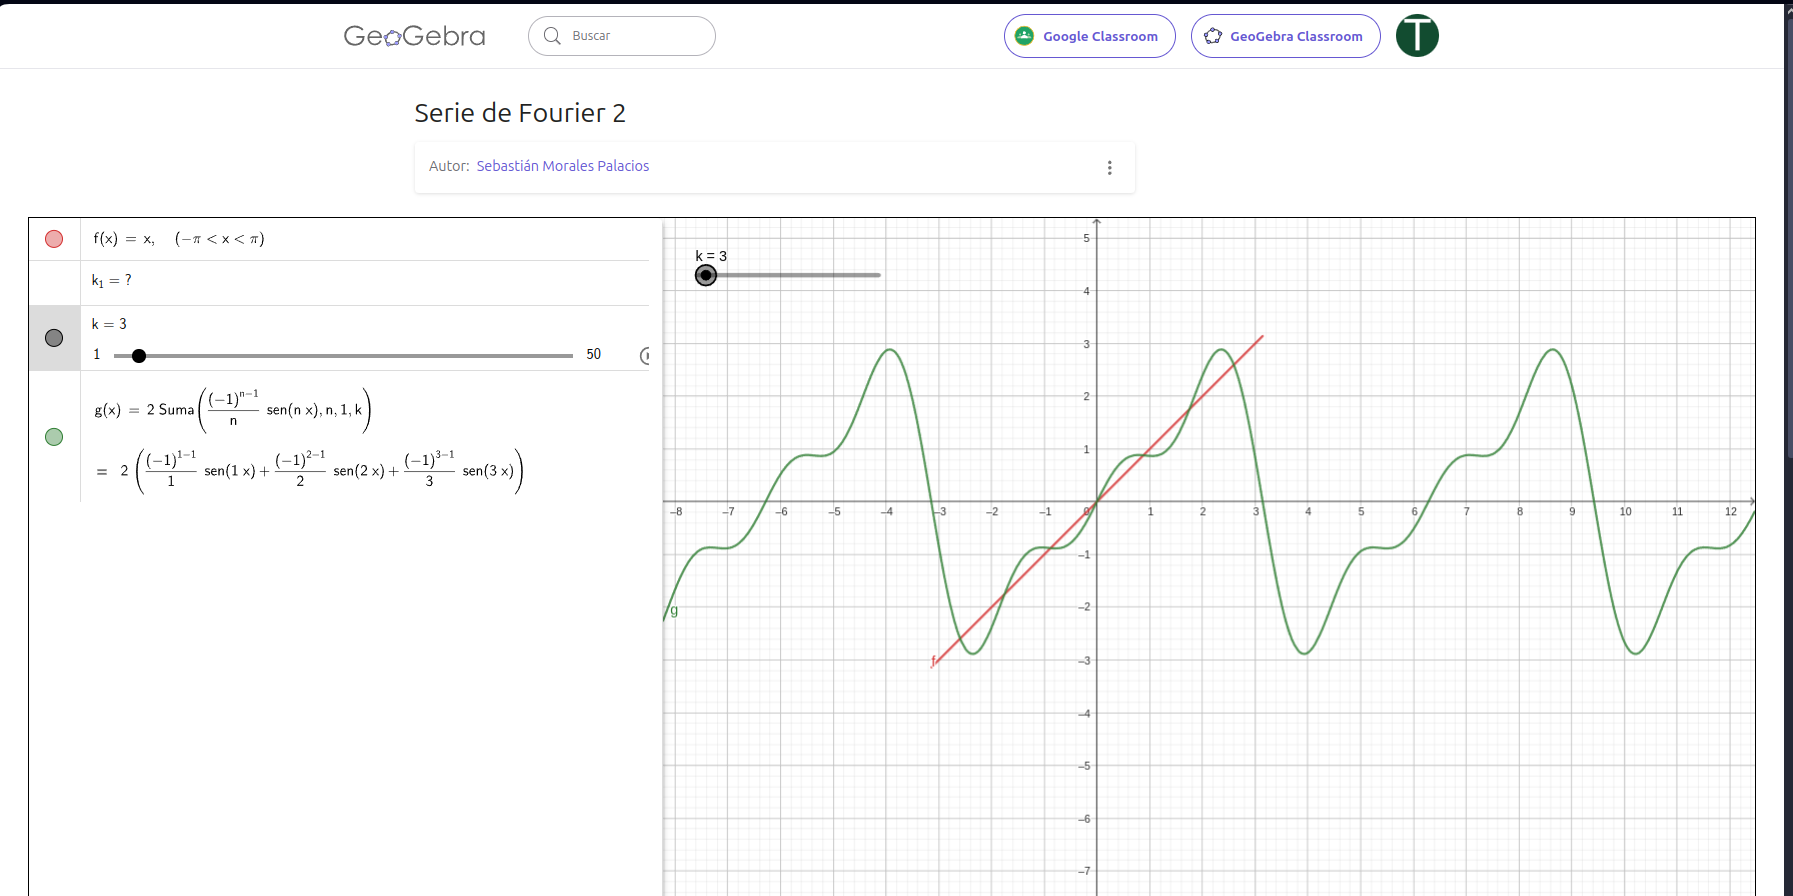
\includegraphics[width=1\textwidth]{img/chapter02/geogebra-trig-series.png}
	\caption{Gráfica de la serie trigonométrica de Fourier en Geogebra}
	\label{fig:geogebra-trig-series}  % Etiqueta para la figura
\end{figure}
Geogebra nos dará una gráfica completamente dinámica pero será un tanto pesada, ya que al añadir más de 5 términos la página comenzará a tener problemas con el dinamismo.

\subsubsection{Prueba Desmos}
Para Desmos será algo más sencillo que en Geogebra, ya que solo tendremos que computar la expresión de la serie sin definir funciones, al terminar de computar la serie nos generará en automático el slider, solo 
\begin{figure}[H]
	\centering
	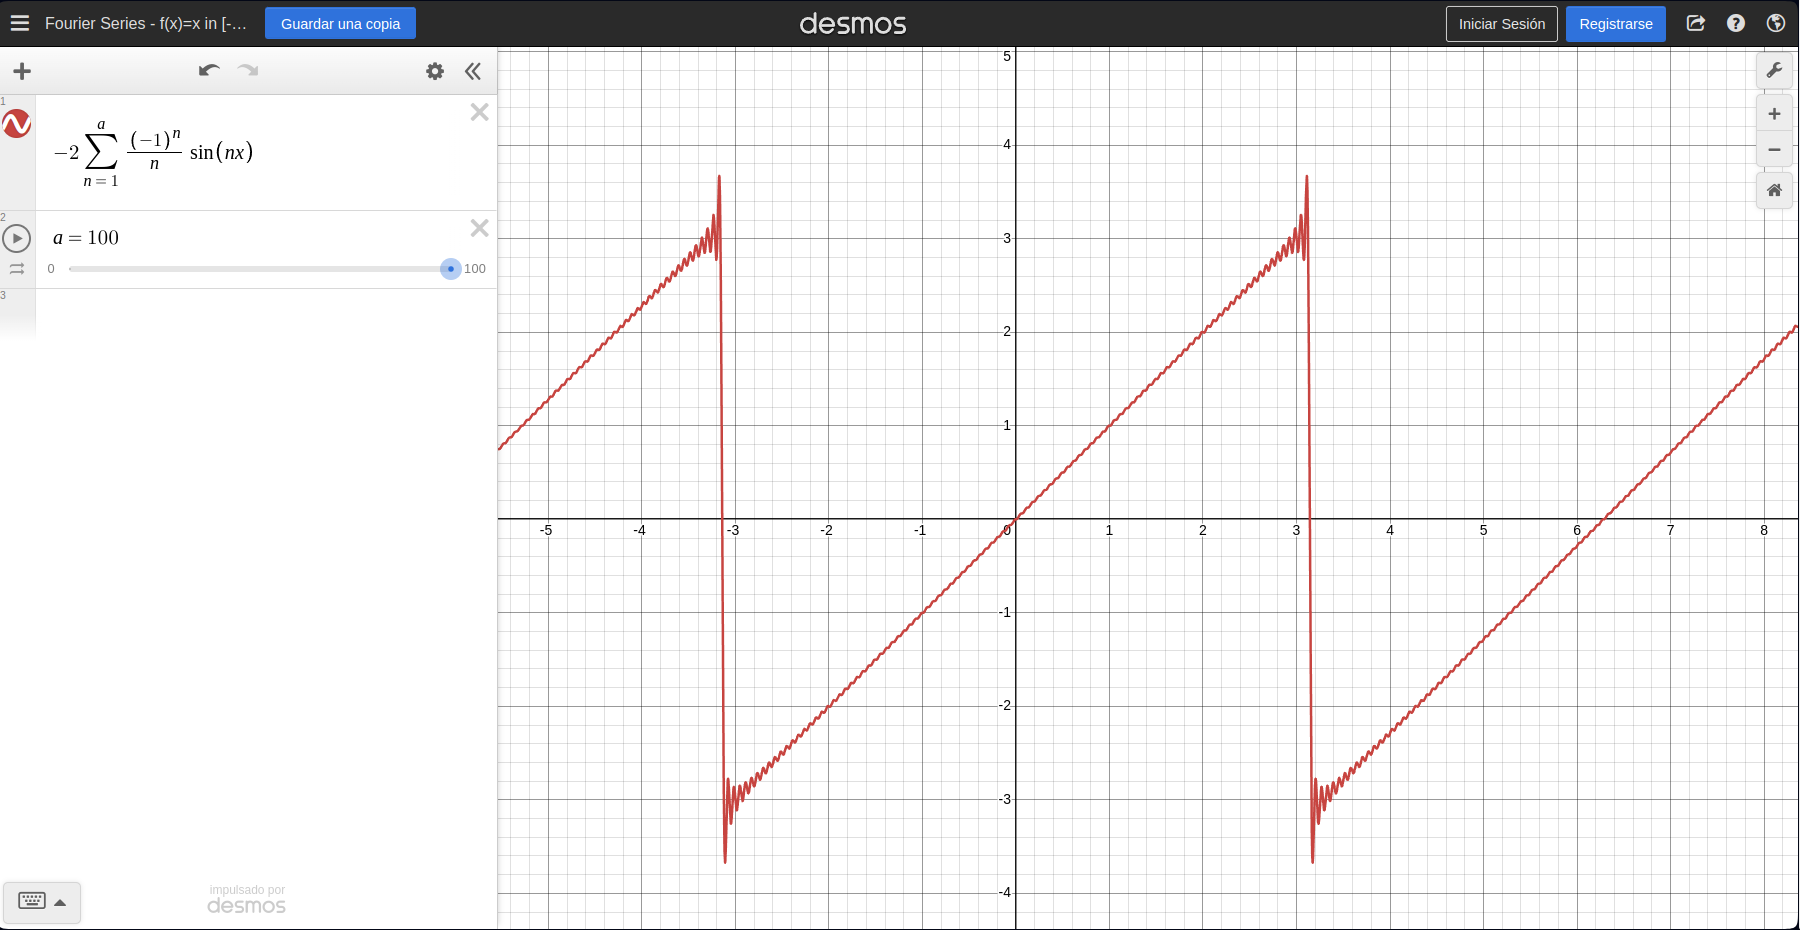
\includegraphics[width=1\textwidth]{img/chapter02/desmos-trig-series-graph.png}
	\caption{Gráfica de la serie trigonométrica de Fourier en Geogebra}
	\label{fig:desmos-trig-series}  % Etiqueta para la figura
\end{figure}
A diferencia de geogebra, la gráfica tendrá un todo un tanto más simple pero será mucho más rápida, ya que podremos hacer una serie con 100 términos y no perderá fluidez como lo haría geogebra.

\subsection{Python}
Python es un lenguaje de programación ampliamente utilizado en las aplicaciones web, el desarrollo de software, la ciencia de datos y el machine learning (ML). Los desarrolladores utilizan Python porque es eficiente y fácil de aprender, además de que se puede ejecutar en muchas plataformas diferentes. El software Python se puede descargar gratis, se integra bien a todos los tipos de sistemas y aumenta la velocidad del desarrollo ~\cite{amazonPython}.
\begin{figure}[H]
	\centering
	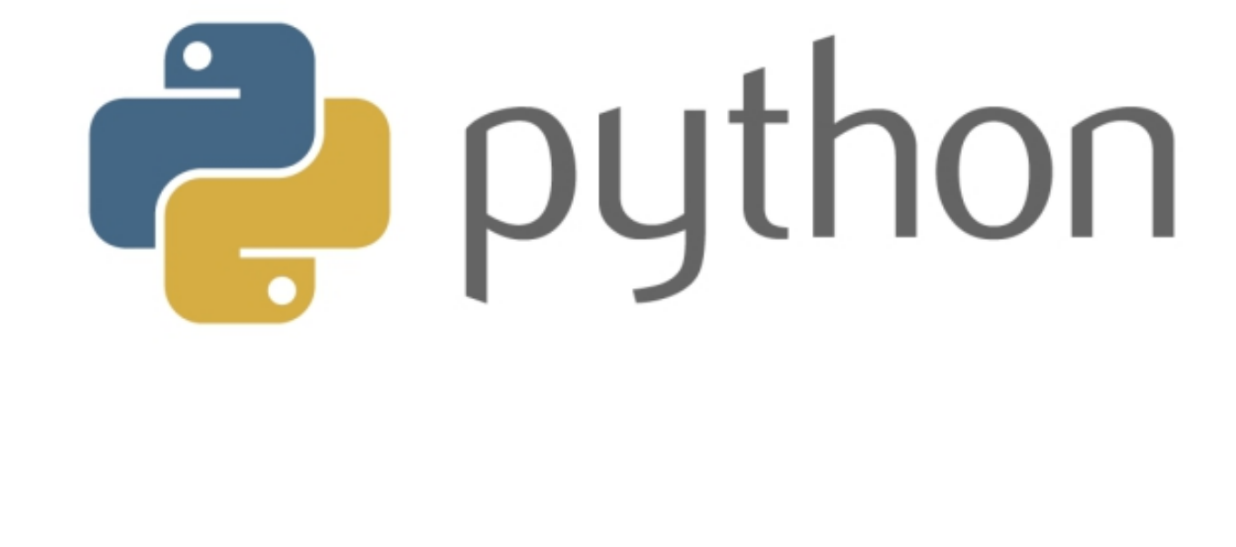
\includegraphics[width=0.3\textwidth]{img/chapter02/logo_python.png}
	\caption{Logo de Python}
	\label{fig:pythonl-ogo}  % Etiqueta para la figura
\end{figure}
La versatilidad de python permiten que se creen bibliotecas para todo tipo de tareas con él, una de ellas es la de hacer cálculos matemáticos y creación de gráficos, de los cuales, podemos tomar funciones especificas para ayudarnos en el calculo de series de Fourier. 

\subsubsection{Sympy / Matplotlib}
SymPy y Matplotlib son dos bibliotecas de Python utilizadas en el dentro de las matemáticas y la visualización de datos. SymPy es una biblioteca de matemáticas simbólicas que permite realizar manipulaciones algebraicas, resolver ecuaciones, derivar e integrar funciones ~\cite{sympy2024}. Por otro lado, Matplotlib es una biblioteca de visualización que permite crear gráficos estáticos, interactivos y animados ~\cite{matplotlib2024}. Al combinar SymPy con Matplotlib, es posible pueden realizar cálculos simbólicos complejos y representar visualmente los resultados de manera clara y efectiva. 
\subsubsection{Prueba Python con Sympy y Matplotlib}
Para este caso, utilizaremos las funciones de integración numérica de Sympy para calcular los coeficientes de la serie trigonométrica y usando las funciones de graficación de Matplotlib, crearemos un gráfico para visualizar la función original con su aproximación de Fourier, para esto usamos el código en \hyperref[app2:complex-code-python-matplotlib-sympy]{Apendice B}. 
\begin{figure}[H]
	\centering
	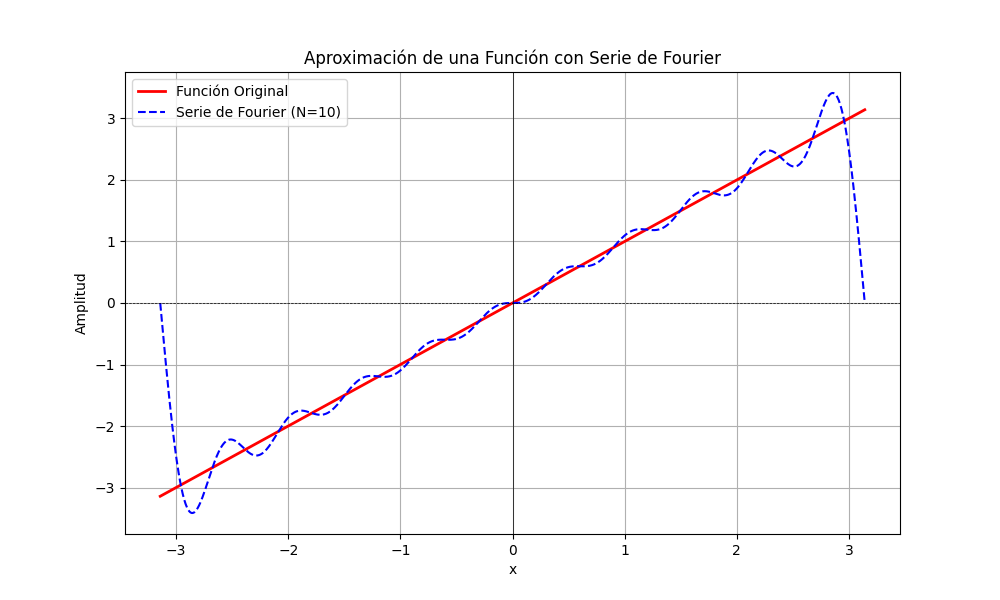
\includegraphics[width=1\textwidth]{img/chapter02/python-sympy-matplotlib.png}
	\caption{Gráfica de la serie trigonométrica y/o exponencial de Fourier en Python con Sympy y Matplotlib}
	\label{fig:python-matplotlib-sympy-trig-series}  % Etiqueta para la figura
\end{figure}
Ahora, si hacemos unos cambios en el código para que calcule el coeficiente de la serie exponencial compleja \hyperref[app2:complex-code-python-matplotlib-sympy], obtendremos exactamente la misma gráfica en \ref{fig:python-matplotlib-sympy-trig-series}, notando que Sympy es capaz de simplificar la parte imaginaria de la serie exponencial compleja para poder ver la parte real resultante en la gráfica.

\subsubsection{Manim}
Manim es una biblioteca de Python de código abierto diseñada para la creación de animaciones matemáticas de alta calidad. Desarrollada inicialmente por Grant Sanderson para su canal de YouTube "3Blue1Brown", Manim permite crear animaciones dinámicas y precisas de manera intuitiva y atractiva. La herramienta ofrece un control detallado sobre cada aspecto de la animación~\cite{Manim2024}.
\subsubsection{Prueba Python con Manim}
Para poder usar a manim, debemos definir toda la expresión de la serie trigonométrica y usar las funciones que nos ofrece manim para hacer la animación como se detalla en el código en \hyperref[app2:trig-code-python-manim]{Apendice B}.
\begin{figure}[H]
	\centering
	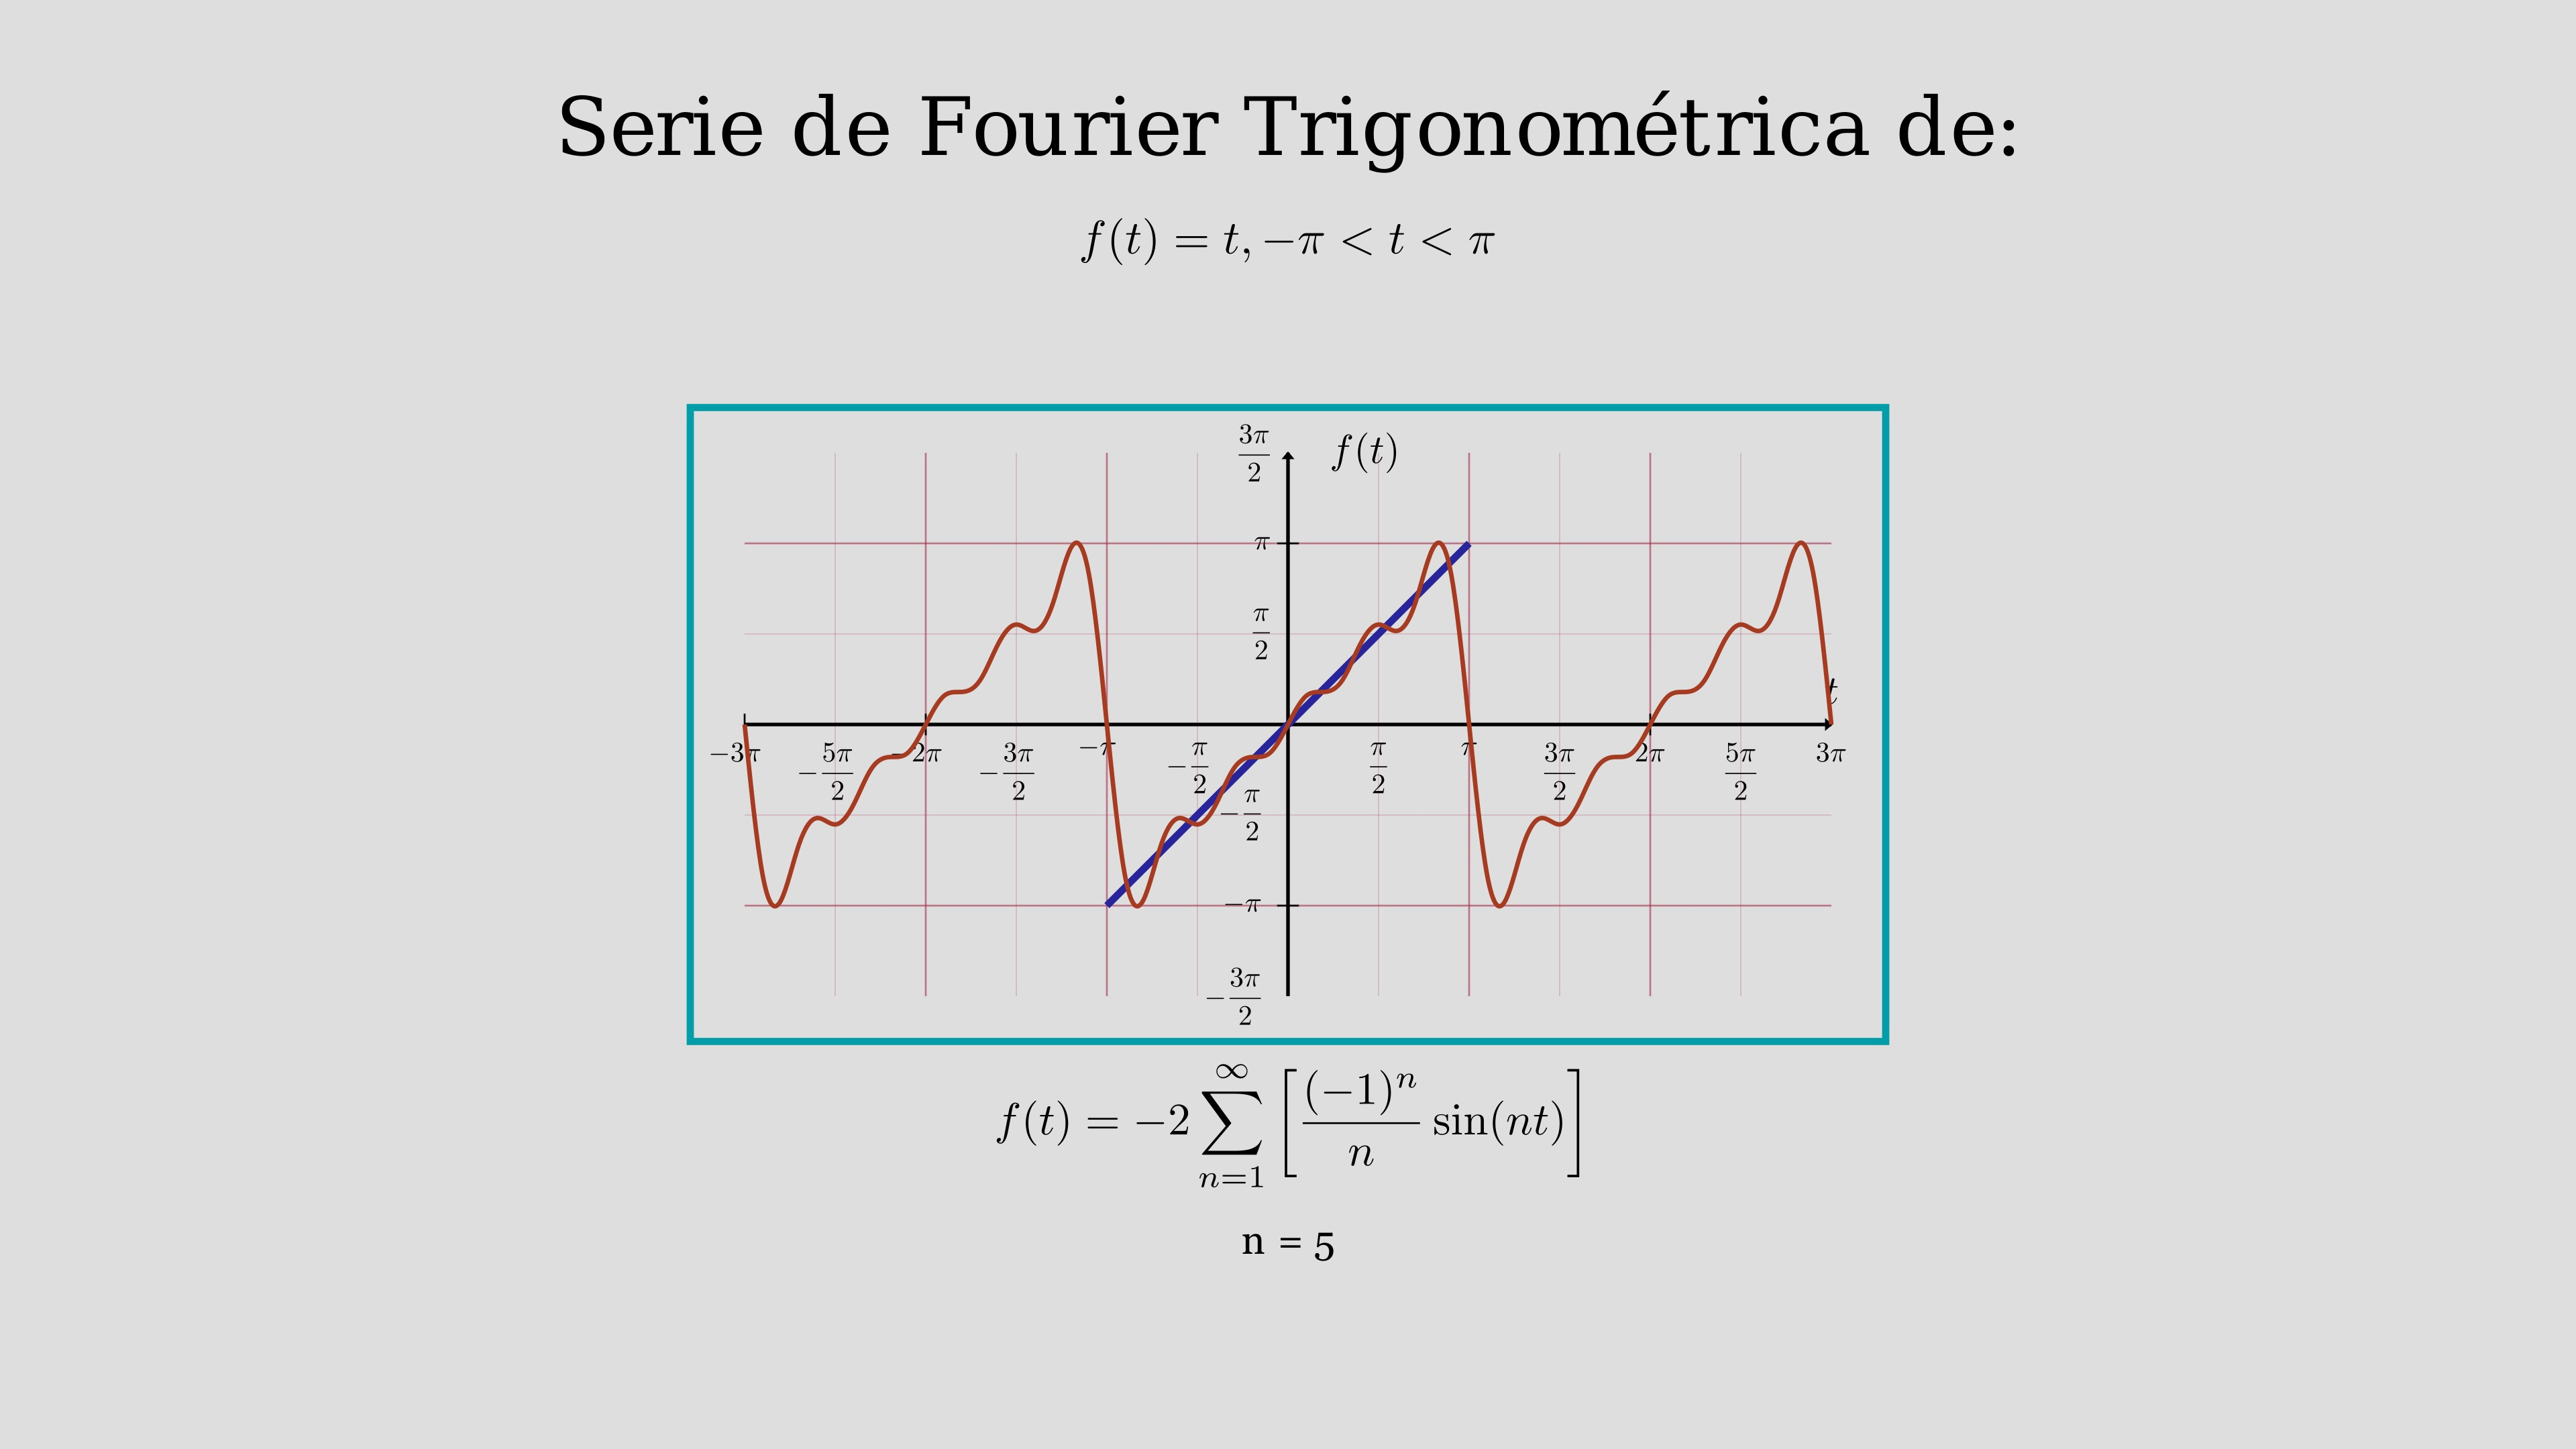
\includegraphics[width=1\textwidth]{img/chapter02/manim-trig-series-graph.jpg}
	\caption{Gráfica de la serie trigonométrica de Fourier en Python con Manim}
	\label{fig:python-manim-trig-series}  % Etiqueta para la figura
\end{figure}
Ahora, ejecutamos el código en \hyperref[app2:complex-code-python-manim]{Apendice B} para la serie compleja y obtenemos la siguiente salida.
\begin{figure}[H]
	\centering
	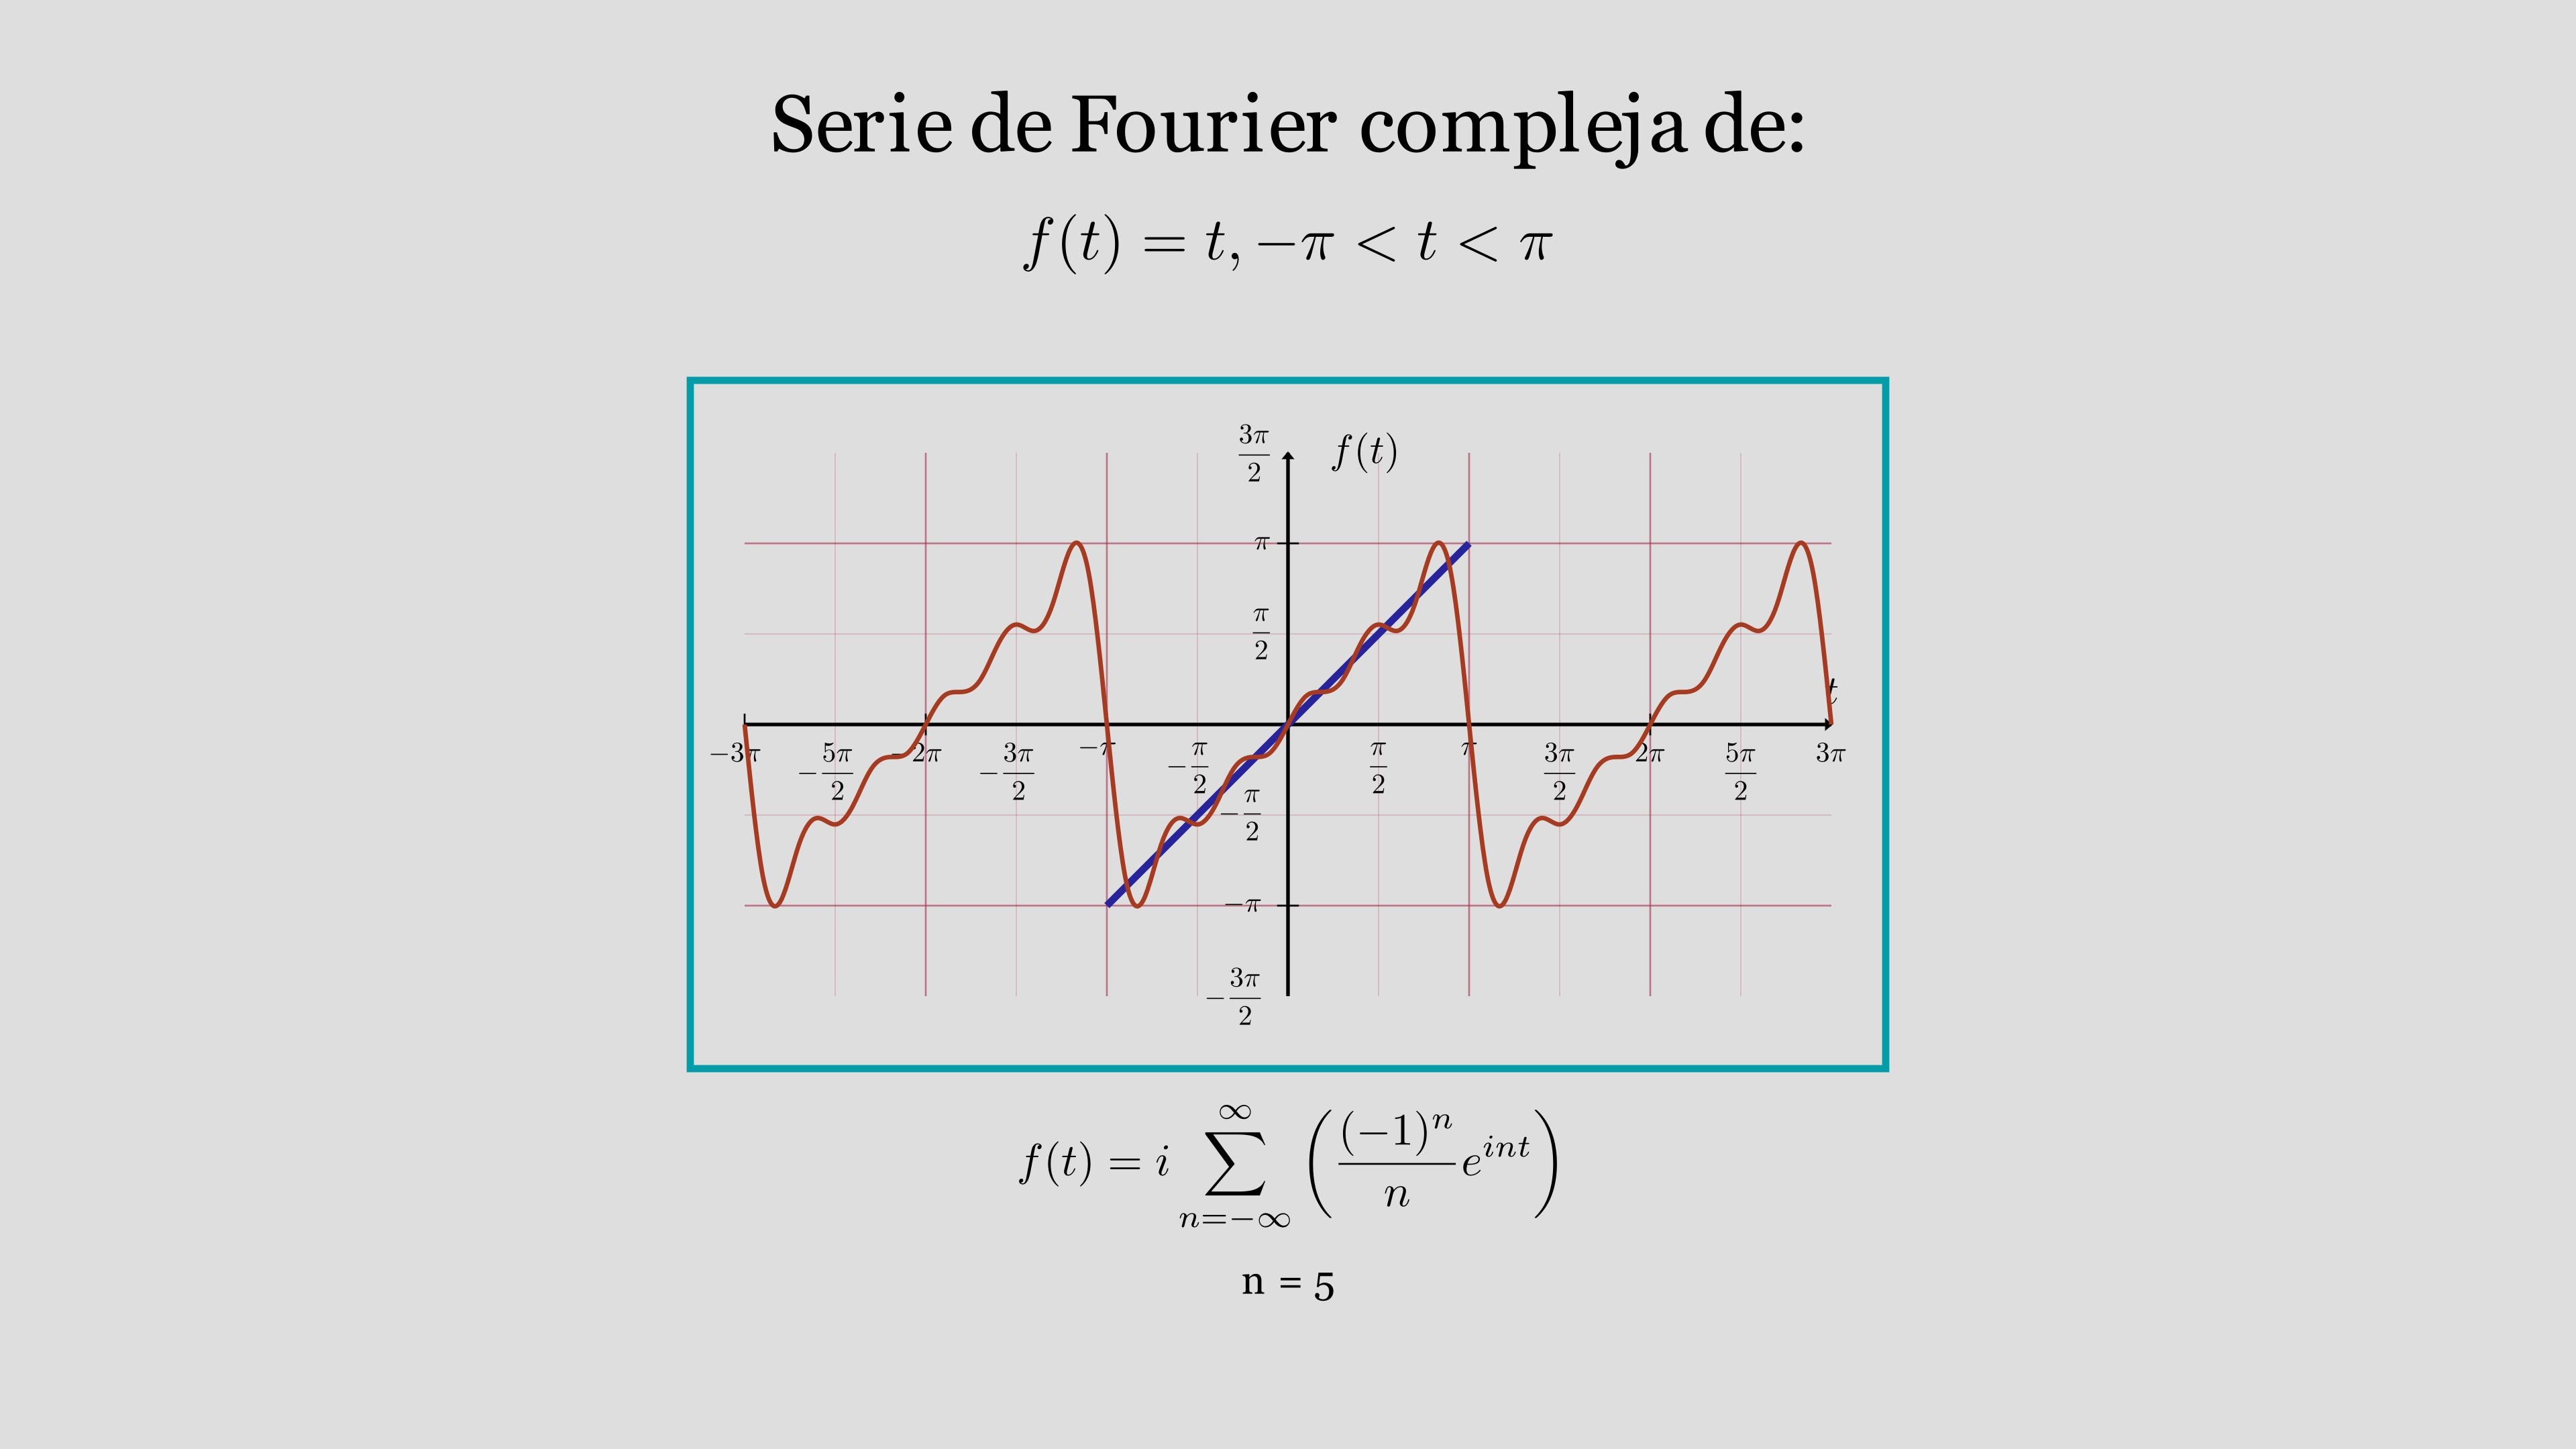
\includegraphics[width=1\textwidth]{img/chapter02/manim-complex-series-graph.jpg}
	\caption{Gráfica de la serie compleja de Fourier en Python con Manim}
	\label{fig:python-manim-complex-series}  % Etiqueta para la figura
\end{figure}
Manim genera gráficas impecables con animaciones fluidas y limpias, sin embargo debemos recordar que los coeficientes deben ser calculados previamente ademas de que tardará bastante tiempo en renderizar el video o imagen dependiendo de la cantidad de calculo que tenga que resolver o la calidad de la imagen.
\section{Comparativa del Funcionamiento de las Herramientas}
En base a la evaluación de cada herramienta, se muestra la tabla \ref{tabla:Comparativa de los sistemas vistos en función de las series de Fourier} a modo de resumen.
\begin{longtable}{ | c | m{6.5cm} | m{4.5cm} | }
	\rowcolor{black!75}
	\head {Herramienta} & \head {Resumen del Funcionamiento} & \head {Costo \newline (Noviembre 2024)} \\ \hline
	\endfirsthead
	\multicolumn{3}{c}{{\tablename\ \thetable{} -- continuación}} \\
	\rowcolor{black!75}
	\head {SOFTWARE} & \head {Resumen del Funcionamiento} & \head {PRECIO} \\ \hline
	\endhead
	\hline \multicolumn{3}{r}{{Continúa en la siguiente página}} \\
	\endfoot
	\hline
	\endlastfoot
	Wolfram Alpha & Con sus funciones especiales para series de Fourier se pueden obtener diferentes expansiones de funciones de un solo trozo o varios, esta función debe ser de un periodo de 2$\pi$, además de mostrar una gráfica estática de la aproximación en serie de Fourier. Para obtener los n-ésimos coeficientes o para funciones de otro periodo, se pueden usar sus funciones de integración.  & Tiene un plan gratuito suficiente para hacer los cálculos. También cuenta con un plan mensual de MXN\$239 que habilita soluciones paso a paso, además de soporte. Está bajo una licencia comercial propietaria. No permite modificación ni redistribución; solo los usuarios que tienen una licencia activa pueden utilizar el software. \\ \hline
	
	Symbolab & Cuenta con una función para calcular la serie trigonométrica de una función de un solo trozo de cualquier periodo. Para otro tipo de series, se pueden usar sus funciones de integración para obtener los resultados & Tiene un plan gratuito suficiente para hacer los cálculos. También cuenta con un plan mensual de MXN\$140 que habilita soluciones paso a paso. Al ser un servicio en linea propietario no permite redistribución o modificación del código ni el software.
	\\ \hline
	
	Matlab & Se puede diseñar un código que integre numéricamente para obtener los coeficientes y luego graficarlos, o tener el resultado y directamente graficarlo. & Tiene licencia gratuita para alumnos de diversas universidades. Fuera de esto, tiene planes desde USD\$99 anuales para estudiantes. Está bajo una licencia comercial propietaria. No permite modificación ni redistribución; solo los usuarios que tienen una licencia activa pueden utilizar el software. \\ \hline
	
	Maple & Si bien no tiene funciones propias para series de Fourier, con sus funciones de integración es posible integrar simbólicamente cualquier función matemática (mientras sea válida) ya sea de uno o varios trozos, para obtener los coeficientes, expandir la serie y reconstruir la gráfica. Aunque tiene problemas para graficar la serie exponencial por los números complejos, si obtiene sus coeficientes. & Cuenta con planes desde USD\$75 para estudiantes. Está bajo una licencia comercial propietaria. No permite modificación, redistribución ni acceso al código fuente. \\ \hline
	
	Maxima & Cuenta con funciones para trabajar con diversos tipos de problemas de series de Fourier, además de que cuenta con funciones de integración simbólica, lo que permite calcular los coeficientes y la expansión trigonométrica y la exponencial de cualquier función matemática (mientras sea válida) ya sea de uno o varios trozos sin problemas,además de poder generar un gráfico. & Es un sistema gratuito bajo la Licencia Pública General (GNU), además de ser de código abierto. \\ \hline
	
	Geogebra & Cuenta con funciones para graficar series de funciones, en las que se puede graficar la serie trigonométrica de forma dinámica, habiendo realizado previamente los cálculos de los coeficientes necesarios & Es un sistema gratuito bajo la Licencia Pública General (GNU), además de ser de código abierto.  \\ \hline
	
	Desmos & Al igual que con Geogebra, cuenta con una función para graficar series de funciones sobre un lienzo dinámico, con la diferencia de tener una interfas mas sencilla y con mayor rendimiento que Geogebra & Es un sistema gratuito bajo la Licencia Pública General (GNU), además de ser de código abierto.  \\ \hline
	
	Matplotlib / Sympy & Si bien estas bibliotecas no tienen funciones propias para trabajar con series de Fourier, es posible crear un programa en pyhton que use las funciones de integración numérica de Sympy para luego hacer una gráfica en matplotlib de la serie de Fourier obtenida. & Ambas son bibliotecas gratuitas licenciadas bajo BSD, además de ser de código abierto. \\ \hline
	
	Manim & Si bien Manim no cuenta con ninguna función de integración, es posible crear un programa en python que genere gráficos como imagen o video de cualquier serie de Fourier, mientras ya hayamos calculado los coeficientes, los recursos que crea son altamente personalizables desde el código  & Es una bibliotecas gratuita bajo la Licencia MIT, además de ser de código abierto. \\ \hline
	
	%\caption{Comparación de software para cálculos matemáticos y visualización de datos} \label{tabla:Comparativa de los sitemas vistos en función de las series de Fourier} \\
\end{longtable}
\captionof{table}{Comparación de software para cálculos matemáticos y visualización de datos} \label{tabla:Comparativa de los sistemas vistos en función de las series de Fourier}
\vspace{0.5cm}



De esta tabla podemos observar que si bien, hay opciones que para calculo simbólico sumamente potentes que nos permiten calcular los coeficientes, estás se ven limitadas en la visualización de generar una gráfica dinámica e intuitiva, mientras que las que ofrecen una mejor visualización de las series en las gráficas no siempre pueden hacer los cálculos o algunas no tienen forma de graficar cuando la serie presenta números complejos, sin mencionar que la mayoría requiere de conocimientos en programación especializado en el lenguaje de la herramienta.

%\section{Trabajos y Proyectos Relacionados}
%En esta sección se analizarán trabajos académicos y proyectos de investigación que han desarrollado herramientas similares o que abordan la enseñanza de series de Fourier y el uso de plataformas interactivas para la educación matemática. 

%\begin{table}[h]
%	\centering
%	\begin{tabular}{ | m{2.5cm} | m{6.5cm} | m{4cm} | }
%		\rowcolor{black!75}
%		\head {SOFTWARE} & \head {CARACTERÍSTICAS} & \head {PRECIO} \\ \hline
%		Wolfram Alpha & Potente motor de conocimiento computacional para cálculos matemáticos y gráficos. No especializado en series de Fourier.~\cite{wolfram2024}  & Desde MXN \$1,200.00 anuales para estudiantes, plan gratuito limitado. \\ \hline
%		Geogebra & Herramienta dinámica para construcciones geométricas y gráficas. Requiere cálculos previos para series de Fourier.~\cite{GeoGebra2024} & Software libre y código abierto \\ \hline
%		Desmos  & Similar a Geogebra es una calculadora gráfica en línea para cálculos y gráficos, incluida la representación de series de Fourier. Requiere cálculos previos para series de Fourier.~\cite{Desmos2024} & Software libre y código abierto\\ \hline
%		Manim & Librería de animación en Python para visualizaciones matemáticas, incluida la animación de series de Fourier. Requiere conocimientos de programación y cálculos previos.~\cite{Manim2024} & Software libre y código abierto \\ \hline
%		Matlab  & Entorno de programación para cálculos numéricos y visualización de datos, con herramientas específicas para series de Fourier. Requiere conocimientos en programación.~\cite{MathWorks2024} & Desde USD\$99 (aprox. MXN\$1627.82) anuales para estudiantes.\\ \hline
%	\end{tabular}
%	\caption{Comparación de software para cálculos matemáticos y visualización de datos}
%	\label{tabla:software}
%\end{table}

	\chapter{Marco Teórico}\label{ch:Marco Teórico}
En este capítulo se presentará la teoría necesaria para el desarrollo de nuestra calculadora de series de Fourier. Comenzaremos explorando la historia y evolución de las series de Fourier, se detallarán las fórmulas matemáticas para comprender la descomposición de funciones periódicas en sumas de senos y cosenos, resaltando los conceptos de coeficientes de Fourier. Además, se presentan las tecnologías necesarias para la elaboración del proyecto.

\section{Origen e historia de las series de Fourier}
Uno de los problemas del que se ocuparon los matemáticos del siglo XVIII es el que se conoce con el nombre del \textit{problema de la cuerda vibrante}. Este problema fue estudiado por D’Alambert y Euler (usando el método de propagación de las ondas) y un poco más tarde, concretamente en 1753, por Daniel Bernoulli. La solución dada por este difería de la proporcionada por los anteriores y consistió básicamente en expresar la solución del problema como superposición (en general infinita) de ondas sencillas. 

Las ideas de Bernoulli fueron aplicadas y perfeccionadas por Fourier, en 1807, en el estudio de problemas relacionados con la conducción del calor. Quedaron plasmadas por escrito en el libro clásico \emph{Théorie analytique de la chaleur}, publicado en 1822. Los razonamientos realizados por Fourier en este libro plantearon de manera inmediata numerosas controversias y cuestiones que han tenido una influencia significativa en la historia de la Matemática ~\cite{historia-alambert-fourier-euler}.

\subsection{El problema de la cuerda oscilante}

Uno de los problemas más interesantes que abordaron los científicos del siglo XVIII, y que aparece con frecuencia en problemas físicos relacionados con procesos oscilatorios, es el conocido como \textit{problema de la cuerda vibrante}. Este se puede describir en su forma más elemental de la siguiente manera: Supongamos que tenemos una cuerda flexible y tensa, cuyos extremos están fijos, convenientemente, en los puntos $(0, 0)$ y $(\ell, 0)$ sobre el eje horizontal. Si la cuerda se tira de modo que su forma inicial corresponde a la curva definida por $y = f(x)$, y luego se suelta, la pregunta es: ¿Cuál será el movimiento resultante de la cuerda?

Los desplazamientos de la cuerda siempre se encuentran en un mismo plano, y el vector desplazamiento es perpendicular en cualquier momento. Para describir este movimiento se utiliza una función $u(x, t)$, donde $u(x, t)$ representa el desplazamiento vertical de la cuerda en la posición $x$ (con $0 \leq x \leq \ell$) y en el instante $t$ (con $t \geq 0$). El problema es determinar $u(x, t)$ a partir de $f(x)$ ~\cite{weinbergerEDP}.

\subsubsection{D’Alambert y Euler}
El primer matemático que propuso un modelo adecuado para este problema fue Jean Le Rond D’Alambert ~\cite{unal_52162}. Bajo diversas hipótesis (asumiendo, por ejemplo, que las vibraciones son "pequeñas"), en 1747 D’Alambert dedujo la ecuación de onda en la siguiente forma:

\begin{equation} \label{eq1}
	\begin{split}
		\frac{\partial^2 u(x,t)}{\partial t^2} &=  \frac{\partial^2 u(x,t)}{\partial x^2}, \quad 0 < x < \ell, \ t > 0 \\
	\end{split}
\end{equation}
en donde:
\begin{itemize}
	\item \( u(x,t) \): Es la función que describe el desplazamiento de la onda en función de la posición \( x \) y el tiempo \( t \).
	\item \( \frac{\partial^2 u(x,t)}{\partial t^2} \): Segunda derivada parcial de \( u(x,t) \) respecto al tiempo \( t \), que representa la aceleración del desplazamiento de la onda.
	\item \( \frac{\partial^2 u(x,t)}{\partial x^2} \): Segunda derivada parcial de \( u(x,t) \) respecto a la posición \( x \), que describe la curvatura espacial de la onda.
\end{itemize}

 y esta debe satisfacer las condiciones siguientes:

\begin{equation} \label{eq2}
	\begin{split}
		u(x,0) &= f(x), \quad 0 \leq x \leq \ell \\
		\frac{\partial u(x,0)}{\partial t} &= 0, \quad 0 \leq x \leq \ell \\
		u(0,t) &= u(\ell,t) = 0, \quad t \geq 0.
	\end{split}
\end{equation}


En donde la primera ecuación establece la posición inicial de la cuerda, mientras que la segunda indica que la velocidad inicial de la cuerda es cero (recordando que, una vez desplazada a la posición $f(x)$, la cuerda es liberada). La última condición expresa que, para cualquier tiempo, los extremos de la cuerda permanecen fijos. En la figura \ref{fig:cuerda-vibrante} La variable $u = u(x,t)$ mide el desplazamiento sobre la vertical a tiempo $t > 0$ en la posición $x \in [0,\ell]$.

\begin{figure}[h]
	\centering
	
	\begin{tikzpicture}[scale=1.0]
		% Ejes coordenados
		\draw[->,ultra thick] (-0.5,0) -- (7,0) node[right] {$x$};
		\draw[->,ultra thick] (0,-1) -- (0,2) node[above] {$u(x,t)$};
		
		% Extremos fijos en x=0 y x=L
		\draw[thick] (0,0) circle (0.05) node[below] {$x=0$};
		\draw[thick] (6,0) circle (0.05) node[below] {$x=\ell$};
		
		% Desplazamiento inicial de la cuerda
		\draw[domain=0:6,smooth,variable=\x,guinda,thick] plot ({\x},{1.8*sin(180*\x/6)});
		
		% Etiqueta de la cuerda
		\node[above,guinda] at (3,1.9) {$u(x,0) = f(x)$};
		
		% Condiciones de contorno (Movidas hacia arriba para evitar superposición)
		\draw[<-] (0,0.1) -- (-0.5,0.4) node[left] {$u(0,t)=0$};
		\draw[<-] (6,0.1) -- (6.5,0.4) node[right] {$u(\ell,t)=0$};
		
		% Indicación de tiempo inicial
		\node at (3,-0.8) {$t = 0$};
		
		% Flecha de tiempo (opcional)
		% \draw[->] (6.5,1) -- (6.5,1.5) node[right] {$t$ aumenta};
	\end{tikzpicture}
	\caption[Ilustración del problema de la cuerda vibrante.] {Ilustración del problema de la cuerda vibrante. \textit{Fuente: Elaboración propia} }
	\label{fig:cuerda-vibrante}  % Etiqueta para la figura
\end{figure}
%https://teorica.fis.ucm.es/pparanda/EDPdf/EDPviejas/ppedp6.pdf

Y apartir de esto, construyó la solución ~\cite{demostracion-onda}:

\begin{equation}\label{eq3}
	u(x,t) =   F\left( x+t \right) + G\left( x-t \right)
\end{equation}

Que, estando sujeta a las condiciones de frontera \ref{eq2} se podía reducir a ~\cite{demostracion-onda}:

\begin{equation}\label{eq4}
	u(x,t) =   F\left( x+t \right) + F\left( x-t \right)
\end{equation}

siempre y cuando la función \( F \) fuese periódica, impar y diferenciable en todas partes. D’Alambert demostraba con esto que la ecuación de onda admitía “un número infinito de soluciones”. \newline 

Euler entra en escena al criticar varias de las suposiciones que D'Alambert hiciera para encontrar su solución. Una de particular interés es la de suponer que la forma inicial de la curva o cuerda era continua y diferenciable “como una anguila”. Esta suposición para Euler, le quitaba generalidad a la solución de D' Alambert pues omitía funciones, notablemente la que representa una cuerda al
ser pulsada, como se muestra en la figura \ref{fig:cuerda-vibrante}.
Euler derivó una ecuación de onda ligeramente más general que la de D'Alembert \ref{eq1}:
\begin{equation}\label{eq5}	
	\frac{1}{c^2} \frac{\partial^2 u(x,t)}{\partial t^2} = \frac{\partial^2 u(x,t)}{\partial x^2} 
\end{equation}

con la solución ~\cite{demostracion-onda}:

\begin{equation}\label{eq6}	
	u(x,t) = F(x+ct) + G(x-ct)
\end{equation}

que con las mismas condiciones de frontera resulta en ~\cite{demostracion-onda}:

\begin{equation}\label{eq7}	
	u(x,t) = F(x+ct) + F(x-ct)
\end{equation}


Euler argumentaba, a diferencia de D'Alembert, que la función \( F \) quedaba determinada por la posición y velocidad inicial de la cuerda. Si denotamos por \( w(x) \) y \( v(x) \) a éstas, respectivamente, entonces la solución puede representarse como:


\begin{equation}\label{eq8}	
	u(x,t) = \frac{1}{2} \left( w(x+ct) + w(x-ct) + \frac{1}{c} \int_{x-ct}^{x+ct} v(s) ds \right)
\end{equation}

Las funciones \( w \) y \( v \) podían ser arbitrarias (en el sentido que podían representar cualquier curva que pudiera “dibujarse a mano”) e incluía, implícitamente, a la curva “triangular” de la figura. Como dicen los autores ~\cite{bernoulli_Mechanics} a D'Alembert no le quitaba el sueño sacrificar realismo físico por pureza matemática; Euler, por el contrario, usaba la realidad física para contraargumentar la generalidad de las soluciones obtenidas por el francés aunque su interés no fuera tanto realismo físico sino la generalidad de las soluciones admitidas por la ecuación de onda.

\subsubsection{Bernoulli}
Otra manera de obtener la solución del problema \ref{eq1}, distinta a la de sus distinguidos interlocutores, fue propuesta por Daniel Bernoulli en 1753 ~\cite{bernoulli_Mechanics} La idea clave es obtener la solución de \ref{eq1} como superposición de ondas más sencillas, concretamente aquellas que son de la forma ~\cite{springer1999Physics}:

\begin{equation}\label{eq9}	
	u(x) = \alpha \sin \frac{\pi x}{\ell} + \beta \sin \frac{2\pi x}{\ell} + \gamma \sin \frac{3\pi x}{\ell} + \delta \sin \frac{4\pi x}{\ell} + \dots
\end{equation}

que incorporaban el hecho experimental de que cualquier modo de vibración de una cuerda puede obtenerse superponiendo modos vibratorios simples representados por cada término. Estas funciones representan, para \( n = 1 \), el modo fundamental, y para \( n > 1 \) , sus armónicos. De esta manera, cualquier vibración de la cuerda puede describirse como una superposición de estos armónicos, como se puede ver en la figura \ref{fig:armonicos_cuerda}.

\begin{figure}[h]
	\centering
	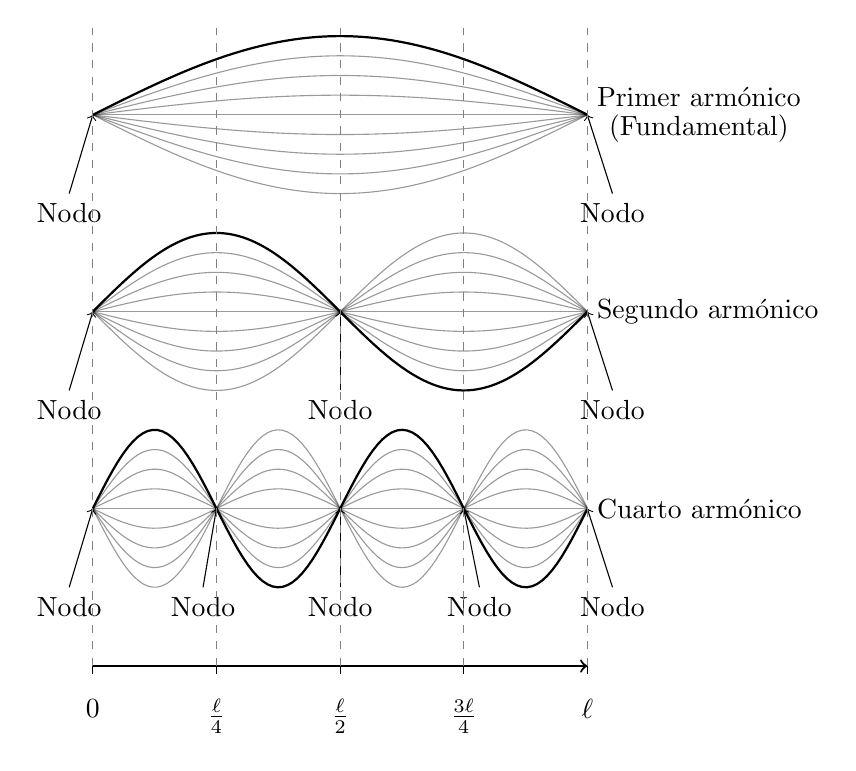
\begin{tikzpicture}[xscale=2]
		
		% Primera onda (n=1)
		\draw[thick] plot[domain=0:3.14, samples=100] (\x,{sin(\x r)});
		\draw [opacity = 0.4] plot[domain=0:3.14, samples=100] (\x,{0.75*sin(\x r)});
		\draw [opacity = 0.4] plot[domain=0:3.14, samples=100] (\x,{0.5*sin(\x r)});
		\draw [opacity = 0.4] plot[domain=0:3.14, samples=100] (\x,{0.25*sin(\x r)});
		\draw [opacity = 0.4] plot[domain=0:3.14, samples=100] (\x,{0*sin(\x r)});
		\draw [opacity = 0.4] plot[domain=0:3.14, samples=100] (\x,{-0.5*sin(\x r)});
		\draw [opacity = 0.4] plot[domain=0:3.14, samples=100] (\x,{-0.25*sin(\x r)});
		\draw [opacity = 0.4] plot[domain=0:3.14, samples=100] (\x,{-0.75*sin(\x r)});
		\draw [opacity = 0.4] plot[domain=0:3.14, samples=100] (\x,{-sin(\x r)});
		\node[right] at (3.14, 0) {\shortstack{Primer armónico \\ (Fundamental)}};
		
		
		\draw[->] (-0.15, -1) node[below] {Nodo} -- (0, 0);
		\draw[->] (3.3, -1) node[below] {Nodo} -- (3.14, 0);
		
		
		% Segunda onda en la parte inferior (misma onda desplazada hacia abajo)
		\begin{scope}[shift={(0,-2.5)}] % Mueve todo el segundo gráfico hacia abajo
			\draw[thick] plot[domain=0:3.14, samples=100] (\x,{sin(2*\x r)});
			\draw [opacity = 0.4] plot[domain=0:3.14, samples=100] (\x,{0.75*sin(2*\x r)});
			\draw [opacity = 0.4] plot[domain=0:3.14, samples=100] (\x,{0.5*sin(2*\x r)});
			\draw [opacity = 0.4] plot[domain=0:3.14, samples=100] (\x,{0.25*sin(2*\x r)});
			\draw [opacity = 0.4] plot[domain=0:3.14, samples=100] (\x,{0*sin(2*\x r)});
			\draw [opacity = 0.4] plot[domain=0:3.14, samples=100] (\x,{-0.5*sin(2*\x r)});
			\draw [opacity = 0.4] plot[domain=0:3.14, samples=100] (\x,{-0.25*sin(2*\x r)});
			\draw [opacity = 0.4] plot[domain=0:3.14, samples=100] (\x,{-0.75*sin(2*\x r)});
			\draw [opacity = 0.4] plot[domain=0:3.14, samples=100] (\x,{-sin(2*\x r)});
			\node[right] at (3.14, 0) {Segundo armónico};
			
			\draw[->] (-0.15, -1) node[below] {Nodo} -- (0, 0);
			\draw[->] (1.57, -1) node[below] {Nodo} -- (1.57, 0);
			\draw[->] (3.3, -1) node[below] {Nodo} -- (3.14, 0);
		\end{scope}
		
		
		% Segunda onda en la parte inferior (misma onda desplazada hacia abajo)
		\begin{scope}[shift={(0,-5)}] % Mueve todo el segundo gráfico hacia abajo
			\draw[thick] plot[domain=0:3.14, samples=100] (\x,{sin(4*\x r)});
			\draw [opacity = 0.4] plot[domain=0:3.14, samples=100] (\x,{0.75*sin(4*\x r)});
			\draw [opacity = 0.4] plot[domain=0:3.14, samples=100] (\x,{0.5*sin(4*\x r)});
			\draw [opacity = 0.4] plot[domain=0:3.14, samples=100] (\x,{0.25*sin(4*\x r)});
			\draw [opacity = 0.4] plot[domain=0:3.14, samples=100] (\x,{0*sin(4*\x r)});
			\draw [opacity = 0.4] plot[domain=0:3.14, samples=100] (\x,{-0.5*sin(4*\x r)});
			\draw [opacity = 0.4] plot[domain=0:3.14, samples=100] (\x,{-0.25*sin(4*\x r)});
			\draw [opacity = 0.4] plot[domain=0:3.14, samples=100] (\x,{-0.75*sin(4*\x r)});
			\draw [opacity = 0.4] plot[domain=0:3.14, samples=100] (\x,{-sin(4*\x r)});
			\node[right] at (3.14, 0) {Cuarto armónico};
			
			% Flechas hacia los nodos
			\draw[->] (-0.15, -1) node[below] {Nodo} -- (0, 0);
			\draw[->] (0.7, -1) node[below] {Nodo} -- (0.785, 0);
			\draw[->] (1.57, -1) node[below] {Nodo} -- (1.57, 0);
			\draw[->] (2.455, -1) node[below] {Nodo} -- (2.355, 0);
			\draw[->] (3.3, -1) node[below] {Nodo} -- (3.14, 0);
		\end{scope}
		
		
		
		\begin{scope}[shift={(0,1)}] 
			% Eje x graduado en múltiplos de pi/4
			\draw[thick, ->] (0,-8) -- (3.14,-8) node[anchor=north] {}; % Eje x
			\foreach \x in {0,0.785,1.57,2.355,3.14} {
				\draw (\x,-8.1) -- (\x,-7.9); % Marcas de tic
			}
			\foreach \x/\label in {0/$0$,0.785/$\frac{\ell}{4}$,1.57/$\frac{\ell}{2}$,2.355/$\frac{3\ell}{4}$,3.14/$\ell$} {
				\draw (\x,-8.3) node[anchor=north] {\label}; % Etiquetas
			}
			
			% Líneas verticales punteadas
			\foreach \x in {0,0.785,1.57,2.355,3.14} {
				\draw[dashed, gray] (\x,-8) -- (\x,0.1); % Líneas punteadas desde el eje x hacia arriba
			}
		\end{scope}
	\end{tikzpicture}
	
	\caption[Ilustración de 3 armónicos y sus nodos de la cuerda al vibrar.] {Ilustración de 3 armónicos y sus nodos de la cuerda al vibrar.\textit{Fuente: Elaboración propia}} 
	\label{fig:armonicos_cuerda}  % Etiqueta para la figura
\end{figure}

Si la solución propuesta por Bernouilli fuese correcta, ello obligaría a que

\begin{equation}\label{eq10}
	u(x, 0) = \sum_{n=1}^{\infty} C_n \sen(nx)
\end{equation}

y por tanto a que

\begin{equation}\label{eq11}
f(x) = \sum_{n=1}^{\infty} C_n \sen(nx), \quad \forall x \in [0, \ell],
\end{equation}

para “una adecuada elección de los coeficientes \( C_n \)”. \newline


Pero esta fórmula no es correcta del todo pues le falta, a cada término, el producto por la función coseno (función del tiempo). Más aún, Bernoulli fue incapaz de mostrar cómo podían obtenerse los coeficientes \( \alpha \), \( \beta \), \( \gamma \), \( \delta \), ... cosa que sí hizo Euler un poco después con el método de integrar la expansión después de multiplicarla por senos o cosenos. Es claro que la solución de Bernoulli no es tan general como la de D’Alembert pero algo que aún el gran Euler no pudo realmente entender es que la solución de Bernoulli permitía funciones iniciales más generales que, a decir de otros autores, fue tema de críticas por parte de Euler a la propuesta de D’Alembert ~\cite{springer1999Physics}.
Bernoulli y Euler mantuvieron una correspondencia epistolar productiva, y se puede afirmar que ambos dependían del otro para realizar su trabajo: Bernoulli necesitaba de Euler para orientar sus estudios matemáticos, mientras que Euler dependía de Bernoulli para comprender los fenómenos físicos que sustentaban su investigación matemática. A pesar de que partían de estudios matemáticos comunes, al final no lograron resolver ni juntos, ni de manera individual, ni desde una perspectiva experimental, donde la matemática jugara un papel metodológico predominante, ni desde el punto de vista matemático donde la física del problema guiara y definiera la teoría. Euler nunca consideró especialmente relevante el trabajo matemático de Daniel Bernoulli, ya que sus métodos eran algo imprecisos, aunque con gran intuición física. Por su parte, Bernoulli tampoco valoraba mucho los estudios matemáticos de Euler, pues estaban distantes de los experimentos. Bernoulli incluso llegó a comentar que Euler "tomaba sus pruebas de la naturaleza y no de algún principio de análisis". ~\cite{springer1999Physics}


\subsection{La ecuación de calor}
Hubo que esperar 54 años hasta que las ideas de Bernoulli fueron tomadas en cuenta por el barón Jean Baptiste-Joseph Fourier, matemático y físico francés, quien, entre otras actividades acompañó a Napoleón, en calidad e científico, en la campaña de éste en Egipto. Allí, como secretario del "Instituto de Egipto", hizo gala de gran competencia en diversos asuntos administrativos. ~\cite{almira2017fourier}

\subsubsection{Fourier}
Al regresar a Francia, y como profesor de Análisis de la Escuela Politécnica, Fourier se interesó por la teoría de la conducción del calor en los cuerpos sólidos. En 1807 envió un artículo a la Academia de Ciencias de París, que trataba sobre dicho tema. Más concretamente, Fourier consideró una varilla delgada de longitud dada \( \ell \), cuyos extremos se mantienen a \( 0^\circ \) centígrados y cuya superficie lateral está aislada. Si la distribución inicial de temperatura en la varilla viene dada por una función \( f(x) \) (se supone que la temperatura de la varilla en cada sección transversal de la misma es constante), ¿Cuál será la temperatura de cualquier punto \( x \) de la varilla en el tiempo \( t \)? Suponiendo que la varilla satisface condiciones físicas apropiadas, Fourier demostró que si \( u(x,t) \) representa la temperatura en la sección \( x \) y en el tiempo \( t \), entonces la función \( u \) debe tener la siguiente forma:

\begin{equation} \label{eq12}
	\begin{split}
		\frac{\partial u(x,t)}{\partial t} &= \alpha^2 \frac{\partial^2 u(x,t)}{\partial x^2} , \quad 0 < x < \ell, \ 0 < t < \infty \\
	\end{split}
\end{equation}

en donde: 
\begin{itemize}
	\item \(\frac{\partial u}{\partial t}(x,t)\): Representa la derivada parcial de \(u\) con respecto al tiempo \(t\), es decir, cómo cambia la temperatura \(u(x,t)\) en el punto \(x\) a lo largo del tiempo \(t\).
	\item \(u(x,t)\): Es la función que describe la temperatura en un punto \(x\) en el espacio y en un tiempo \(t\). Depende tanto de la posición espacial \(x\) como del tiempo \(t\).
	
	\item \(\alpha^2\): Es el coeficiente de difusión térmica, que depende del material en cuestión. Este coeficiente es constante y está relacionado con la capacidad del material para difundir el calor. La unidad de \(\alpha\) es metros cuadrados por segundo \((\text{m}^2/\text{s})\).
	\item \(\frac{\partial^2 u}{\partial x^2}(x,t)\): Representa la derivada parcial segunda de \(u\) con respecto a la posición \(x\), es decir, cómo cambia la pendiente (o curvatura) de la temperatura a lo largo del espacio. Esta cantidad indica cómo el calor se distribuye espacialmente.
\end{itemize}

Esta ecuación modela la difusión del calor en un medio a lo largo del tiempo. La derivada en el tiempo \(\left(\frac{\partial u}{\partial t}\right)\) está relacionada con la derivada segunda en el espacio \(\left(\frac{\partial^2 u}{\partial x^2}\right)\), lo que refleja que el cambio en la temperatura con el tiempo depende de cómo está distribuido el calor en el espacio.
y esta debe satisfacer las siguientes condiciones:

\begin{equation} \label{eq13}
	\begin{split}
		u(0,t) &= u(\ell,t) = 0, \quad 0 \leq t \leq \infty \\
		u(x,0) &= f(x), \quad 0 \leq x \leq \ell.
	\end{split}
\end{equation}

\begin{figure}[h]
	\centering
	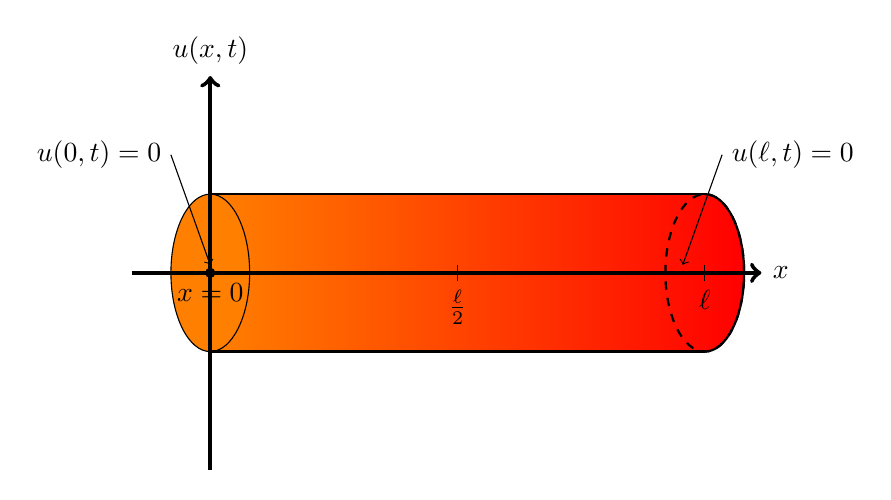
\begin{tikzpicture}
		% Aplicar un sombreado degradado del cilindro (de naranja a rojo)
		\shade[left color=orange, right color=red] (0,1) -- (6.28,1) arc (90:-90:0.5 and 1) -- (0,-1) arc (-90:90:0.5 and 1);
		
		\filldraw [color=orange, draw=black](0,0) ellipse (0.5 and 1);  % Parte delantera del cilindro
		%\shade[left color=orange, right color=red] (0,0) ellipse (0.5 and 1);
		
		% Dibujar las líneas laterales con degradado
		\draw[thick, draw=black] (0,1) -- (6.28,1);
		\draw[thick, draw=black] (0,-1) -- (6.28,-1);
		\draw[thick, draw=black] (6.28,1) arc (90:-90:0.5 and 1);  % Arco frontal
		\draw[dashed, thick, draw=black] (6.28,0) ellipse (0.5 and 1);  % Parte trasera del cilindro
		
		% Dibujar el plano coordenado xy
		\draw[->,ultra thick] (-1,0) -- (7,0) node[right] {$x$};  % Eje x
		\draw[->,ultra thick] (0,-2.5) -- (0,2.5) node[above] {$u(x,t)$};  % Eje y
		
		% Extremos fijos en x=0 y x=L
		\draw[thick] (0,0) circle (0.05) node[below] {$x=0$};
		\draw (3.14,0.1) -- (3.14,-0.1) node[below] {$\frac{\ell}{2}$};
		\draw (6.28,0.1) -- (6.28,-0.1) node[below] {$\ell$};
		
		% Condiciones de contorno (Movidas hacia arriba para evitar superposición)
		\draw[<-] (0,0.1) -- (-0.5,1.5) node[left] {$u(0,t)=0$};
		\draw[<-] (6,0.1) -- (6.5,1.5) node[right] {$u(\ell,t)=0$};
	\end{tikzpicture}
 	\caption[Ilustración del problema de transferencia de calor en una barra de longitud $\ell$.  ]{ Ilustración del problema de transferencia de calor en una barra de longitud $\pi$.  \textit{ Fuente: Elaboración propia} }
	\label{fig:barra-pi}  % Etiqueta para la figura
\end{figure}

La primera condición en \ref{eq12} es una Ecuación en Derivadas Parciales de segundo orden, conocida con el nombre de Ecuación del Calor. La segunda significa que la temperatura, en los extremos de la varilla, se mantiene a \( 0^\circ \) centígrados en cualquier tiempo, mientras que la última relación representa la distribución inicial de temperatura en la varilla considerada.

Partiendo de las ideas de Bernoulli, para la ecuación de ondas, Fourier buscó las soluciones más sencillas que puede presentar la ecuación del calor: aquellas que son de la forma:
\begin{equation} \label{eq14}
	\begin{split}
		u(x,t) = X(x)P(t) \\
	\end{split}
\end{equation}

 Imponiendo la condición de que tales funciones satisfagan, formalmente, dicha ecuación, obtenemos, como en el caso de la ecuación de ondas, los dos problemas siguientes de ecuaciones diferenciales ordinarias ~\cite{demostracion-calor}:
\begin{equation} \label{eq15}
	\begin{split}
		X''(x) + \mu X(x) &= 0, \quad x \in (0, \ell), \ X(0) = X(\ell) = 0 \\
		P'(t) + \mu P(t) &= 0, \quad t > 0
	\end{split}
\end{equation}

Utilizando el método de separación de variables ~\cite{demostracion-calor-feldman}, Fourier propuso que la solución a la ecuación del calor podría expresarse como el producto de dos funciones, una dependiente de la posición \( X(x) \) y otra del tiempo \( P(t) \), como se indica en \eqref{eq13}. Esto descompone la ecuación en dos ecuaciones diferenciales ordinarias: una espacial \eqref{eq15} y una temporal \eqref{eq15}. Fourier resolvió cada una de estas ecuaciones por separado. La solución espacial \( X(t) \) resulta en una serie de funciones sinusoidales que satisfacen las condiciones de frontera en los extremos de la varilla, mientras que la solución temporal \( P(t) \) resulta en exponentes negativos que representan la disipación de calor en el tiempo. Así, disponemos de un procedimiento que nos permite calcular infinitas “soluciones elementales” de la ecuación del calor, a saber, las funciones de la forma \( b_n v_n \), donde \( v_n \) se define como:

\begin{equation} \label{eq16}
	\begin{split}
		v(x,t) = \sin \left( \frac{n \pi}{\ell} x \right) e^{- \alpha^2 \frac{n^2 \pi^2}{\ell^2} k t}
	\end{split}
\end{equation}

Es trivial que, si la distribución inicial de temperatura, \( f \), es algún múltiplo de \( \sen(nx) \) (o una combinación lineal finita de funciones de este tipo), entonces la solución buscada de \eqref{eq16} es un múltiplo adecuado de \( v_n \) (respectivamente, una adecuada combinación lineal de funciones de esta forma).

Ahora bien, \( f(x) \) no es, en general, de la forma justo mencionada, pero, y aquí demostró Fourier, como Bernouilli, una enorme intuición, ¿Será posible obtener la solución \( u(x,t)\) de \eqref{eq16}, para cualquier \( f(x)\) dada, como superposición de las anteriores soluciones sencillas \( v_n \)? Es decir, ¿Será posible elegir adecuadamente los coeficientes \( b_n \) tal que la única solución de \eqref{eq16} sea de la forma:

 
\begin{equation} \label{eq17}
	\begin{split}
		u(x,t) = \sum_{n=1}^{\infty} b_n \sin \left( \frac{n \pi}{\ell} x \right) e^{- \alpha^2 \frac{n^2 \pi^2}{\ell^2} k t}
	\end{split}
\end{equation}

Fourier afirmó en su artículo que esto era correcto. Observemos que nuevamente llegamos a que, entonces, se debe satisfacer la relación \eqref{eq9}. Esto plantea la misma cuestión para dos problemas completamente distintos, el problema \eqref{eq1} y el problema \eqref{eq12}, en donde los coeficientes  \( b_n \) toman la forma:

\begin{equation} \label{eq18}
	\begin{split}
		b_n = \frac{2}{\ell} \int_0^{\ell} f(x) \sin \left( \frac{n \pi x}{\ell} \right) \, dx
	\end{split}
\end{equation}

Los coeficientes \( b_n \) se determinan en función de la distribución inicial de temperatura \( f(x) \) a través de la expresión en \eqref{eq18}, lo que permite que la solución refleje la distribución inicial específica de la varilla. Así, la solución general toma la forma de una serie de Fourier, como se observa en \eqref{eq17}, donde cada término de la serie combina una función sinusoidal en el espacio con un decaimiento exponencial en el tiempo. \newline

El artículo Fourier fue evaluado por Lagrange, Laplace y Legendre y fue rechazado por la Academia Francesa, principalmente debido a la forma en que dedujo la ecuación del calor y por la falta de rigor en sus conclusiones (según la opinión de los académicos mencionados). Sin embargo, los miembros de dicha institución reconocían la relevancia de los problemas relacionados con la propagación del calor, y los resultados teóricos que Fourier presentó mostraban gran concordancia con varios experimentos realizados previamente ~\cite{historia-alambert-fourier-euler}. 

Debido a esto, la Academia estableció un premio sobre el tema. Dicho premio fue otorgado a Fourier en 1812, pero, a pesar de esto, los académicos continuaron criticando la falta de rigor, de modo que, aunque ganó el premio, Fourier no logró publicar su trabajo en la famosa serie “\textit{Mémoires}” de la Academia Francesa. Con gran perseverancia, Fourier continuó trabajando en el tema, y en 1822 publicó su célebre libro \textit{Théorie Analytique de la Chaleur, Firmin Didot, Père et Fils, 1822, París}, donde incluyó gran parte de su artículo de 1812 casi sin modificaciones. Este libro es actualmente una de las obras clásicas en matemáticas ~\cite{historia-alambert-fourier-euler}.

Dos años después, obtuvo el puesto de Secretario de la Academia Francesa, lo que le permitió finalmente publicar su artículo en la serie “\textit{Mémoires}” ~\cite{historia-alambert-fourier-euler}.

\section{Series de Fourier}
Luego de que las soluciones para la ecuación de onda y de calor fueron desarrolladas, Joseph Fourier propuso un nuevo método para expresar funciones periódicas en función de sinusoides. Las bases de lo que hoy conocemos como series de Fourier fueron establecidas por esta propuesta.\newline

A continuación, se describen los conceptos matemáticos en los cuales se basan las series de Fourier, ofreciendo una base firme para entenderlas y aplicarlas en el estudio de funciones que se repiten periódicamente.
\subsection{Funciones Periódicas}
Una función es llamada \textit{función periódica} si existe una constante \( T > 0\) tal que

\begin{equation} \label{eq19}
	\begin{split}
		f(t) = f(t \pm T)
	\end{split}
\end{equation}
para todo valor de \( t \) en el dominio de definición de $f(t)$, donde la constante \( T \) se denomina \textit{periodo} de la función. El periodo también se puede definir como el tiempo transcurrido entre dos puntos equivalentes de una función ~\cite{fourierTolstov}.

Las funciones periódicas aparecen en muchas aplicaciones de matemáticas para problemas de física e ingeniería. Es evidente que la suma, diferencia, producto o cociente de dos funciones con período $T$ también será una función con período $T$ ~\cite{fourierTolstov}.

Si graficamos una función periódica $f(t)$ en un intervalo cerrado $a \leq t \leq a \pm T$, podemos obtener la gráfica completa de $f(t)$ repitiendo periódicamente la porción de la gráfica correspondiente a $a \leq t \leq a \pm T$ \ref{fig:funcion-periodica}.

\begin{figure}[H]
	\centering
	\begin{tikzpicture}[scale=1]
		\begin{axis}[
			axis lines=middle,
			enlargelimits=false,
			width=15cm,
			height=7cm,
			ylabel={\large $f(t)$},
			xlabel={\large $t$},
			xtick={-4*pi, -2*pi, 0, 2*pi, 4*pi},
			xticklabels={$a - 2T$, $a - T$, $a$, $a + T$, $a + 2T$},
			ymin=-4, ymax=4,
			xmin=-4*pi, xmax=4*pi,
			samples=400,
			domain=-4*pi:4*pi,
			axis background/.style={fill=white},
			yticklabels={}, 
			grid=none,
			xticklabel style={yshift=-3cm} % Ajusta el valor según necesites
			]
			
			
			\addplot[guinda, ultra thick] {2 * ((-1)^(1-1)/1 * sin(deg(1*x)) + (-1)^(2-1)/2 * sin(deg(2*x)) + (-1)^(3-1)/3 * sin(deg(3*x)))};    
			
			\addplot[dashed, black, thick] coordinates {(2*pi, -4) (2*pi, 4)};
			\addplot[dashed, black, thick] coordinates {(-2*pi, -4) (-2*pi, 4)};
			\addplot[dashed, black, thick] coordinates {(4*pi, -4) (4*pi, 4)};
			\addplot[dashed, black, thick] coordinates {(-4*pi, -4) (-4*pi, 4)};
			
		\end{axis}
	\end{tikzpicture}
	
		\caption[Gráfica de una función periódica $f(t)$ con periodo $T$.]  {Gráfica de una función periódica $f(t)$ con periodo $T$.\textit{ Fuente: Elaboración propia} }
	\label{fig:funcion-periodica}  % Etiqueta para la figura
\end{figure}
Si $T$ es un período de la función $f(t)$, entonces los números $2T$, $3T$, $4T$, $\dots$ también son períodos. Esto se deduce fácilmente al inspeccionar la gráfica de una función periódica o a partir de la serie de igualdades ~\cite{fourierHsu}
\begin{equation} \label{eq20}
	\begin{split}
		f(t) = f(t \pm T) = f(t \pm 2T) = f(t \pm 3T) = \dots f(t \pm nT), \quad n = 0, \pm1, \pm2, \dots
	\end{split}
\end{equation}
que se obtiene mediante el uso repetido de la condición \eqref{eq19}. Así, si \( T \) es un periodo, también lo es \( nT \), donde \( n \) es cualquier entero positivo, es decir, si existe un periodo, no es único ~\cite{fourierHsu}. Ademas, podemos definir como el \textit{periodo fundamental} \( T_0 \) de \( f(t) \) a el valor positivo más pequeño de \( T \) para el cual se satisface \eqref{eq19}. ~\cite{fourierCinvestav} \newline

Ahora, consideremos la siguiente propiedad de cualquier función \( f(t) \) con período \( T \):

Si \( f(t) \) es integrable en cualquier intervalo de longitud \( T \), entonces es integrable en cualquier otro intervalo de la misma longitud, y el valor de la integral es el mismo. Es decir,

\begin{equation} \label{eq21}
	\int_a^{a+T} f(t) \, dx = \int_b^{b+T} f(t) \, dt
\end{equation}

para cualquier \( a \) y \( b \).

Esta propiedad es una consecuencia directa de la interpretación del área bajo la curva como la integral. De hecho, cada integral de la ecuación anterior representa el área entre la curva \( f(t) \), el eje \( t \), y las líneas verticales en los puntos extremos del intervalo. Las áreas sobre el eje \( t \) se consideran positivas y las áreas bajo el eje \(t\) como negativas. En este caso, las áreas representadas por ambas integrales son iguales debido a la periodicidad de \( f(t) \) ~\cite{fourierTolstov} \ref{fig:area-periodica}.

\begin{figure}
	
	\begin{tikzpicture}[scale=1]
		\begin{axis}[
			axis lines=middle,
			enlargelimits=false,
			width=15cm,
			height=7cm,
			ylabel={\large $f(t)$},
			xlabel={\large $t$},
			xtick={-5*pi/2, -pi/2, pi/4, 9*pi/4},
			xticklabels={\large $a$, $a + T$, $b$, $b + T$},
			ymin=-4, ymax=4,
			xmin=-3*pi, xmax=3*pi,
			samples=400,
			domain=-3*pi:3*pi,
			axis background/.style={fill=white},
			yticklabels={}, 
			grid=none,
			xticklabel style={yshift=-3.2cm, xshift=0} % Ajusta el valor según necesites
			]
			
			% Colorear el área bajo la curva entre a y a+T con patrón
			\addplot [
			draw=none,
			pattern=north east lines, % <-- Cambia fill por pattern
			pattern color=blue,       % <-- Define el color del patrón
			domain=-5*pi/2:-pi/2,
			samples=400,
			] {2 * ((-1)^(1-1)/1 * sin(deg(1*x)) + (-1)^(2-1)/2 * sin(deg(2*x)) + (-1)^(3-1)/3 * sin(deg(3*x)))} \closedcycle;
			
			% Colorear el área bajo la curva entre b y b+T con patrón
			\addplot [
			draw=none,
			pattern=north west lines, % <-- Cambia fill por pattern
			pattern color=red,        % <-- Define el color del patrón
			domain=pi/4:9*pi/4,
			samples=400,
			] {2 * ((-1)^(1-1)/1 * sin(deg(1*x)) + (-1)^(2-1)/2 * sin(deg(2*x)) + (-1)^(3-1)/3 * sin(deg(3*x)))} \closedcycle;
			
			\addplot[guinda, ultra thick] {2 * ((-1)^(1-1)/1 * sin(deg(1*x)) + (-1)^(2-1)/2 * sin(deg(2*x)) + (-1)^(3-1)/3 * sin(deg(3*x)))};    
			
			\addplot[dashed, black, thick] coordinates {(-5*pi/2, -4) (-5*pi/2, 4)};
			\addplot[dashed, black, thick] coordinates {(-pi/2, -4) (-pi/2, 4)};
			\addplot[dashed, black, thick] coordinates {(pi/4, -4) (pi/4, 4)};
			\addplot[dashed, black, thick] coordinates {(9*pi/4, -4) (9*pi/4, 4)};
			
		\end{axis}
	\end{tikzpicture}
	\caption[Gráfica del área bajo la curva de $f(t)$ entre los intervalos desde $a$ hasta $a + T$ y desde $b$ hasta $b + T$. ]{Gráfica del área bajo la curva de $f(t)$ entre los intervalos desde $a$ hasta $a + T$ y desde $b$ hasta $b + T$. \textit{ Fuente: Elaboración propia} }
	\label{fig:area-periodica}  % Etiqueta para la figura
\end{figure}

A partir de ahora, cuando afirmemos que una función \( f(t) \) de período \( T \) es integrable, queremos decir que es integrable en un intervalo de longitud \( T \). Esto implica, a partir de la propiedad recién demostrada, que \( f(t) \) es integrable en cualquier intervalo de longitud finita ~\cite{fourierTolstov}. \newline

Las funciones periódicas más representativas son las funciones trigonométricas \(\sin(t)\) y \(\cos(t)\), ambas con periodo \( T = 2\pi \) (Figura \ref{fig:sen-cos}). Por lo tanto, de acuerdo con \eqref{eq19}, se tiene que \(\sin(t + 2\pi) = \sin(t)\) y \(\cos(t + 2\pi) = \cos(t)\) ~\cite{fourierCinvestav}.

\begin{figure}[H]
	
	\begin{minipage}{0.5\textwidth} % Reducimos el ancho al 48%
		\begin{tikzpicture}[scale=0.46]
			\begin{axis}[
				axis lines=middle,
				grid=both,
				enlargelimits=false,
				width=15cm, % Ancho de la gráfica
				height=13cm, % Altura de la gráfica
				xlabel={\Huge $t$},
				ylabel={\Huge $f(t) = A \sin(t)$},
				xtick={0, 1.5708, 3.1416, 4.7124, 6.2832, 7.8540, 9.4248, 10.9956, 12.5664},
				xticklabels={$0$, $\frac{\pi}{2}$, $\pi$, $\frac{3\pi}{2}$, $2\pi$, $\frac{5\pi}{2}$, $3\pi$, $\frac{7\pi}{2}$, $4\pi$},
				xticklabel style={font=\LARGE},
				ytick={-1.5, -1, -0.5, 0, 0.5, 1, 1.5}, % Gradación de 0.5 en 0.5 en el eje y
				yticklabel style={font=\LARGE},
				ymin=-1.5, ymax=1.5,
				xmin=0, xmax=4*pi,
				samples=400,
				domain=0:4*pi,
				axis background/.style={fill=white}
				]
				
				\addplot[guinda, ultra thick] {( sin(180*x/pi) )};
				
				\addplot[dashed, black, thick] coordinates {(2*pi, -1.5) (2*pi, 1.5)};
				\draw[<->, ultra thick, red] (0,-1.25) -- (2*pi,-1.25) node[midway, below, black] {\LARGE $T$};
				\draw[<->, ultra thick, red] (3*pi/2,0) -- (3*pi/2,-1) node[midway, below right, black, xshift=0.1cm] {\LARGE $A$};
			\end{axis}
		\end{tikzpicture}
	\end{minipage}
	\hspace{0.1cm} % Espacio de 0.5 cm entre las gráficas
	\begin{minipage}{0.5\textwidth} % Reducimos el ancho al 48%
		\begin{tikzpicture}[scale=0.46]
			\begin{axis}[
				axis lines=middle,
				grid=both,
				enlargelimits=false,
				width=15cm, % Ancho de la gráfica
				height=13cm, % Altura de la gráfica
				xlabel={\Huge $t$},
				ylabel={\Huge $f(t) = A \cos(t)$},
				xtick={0, 1.5708, 3.1416, 4.7124, 6.2832, 7.8540, 9.4248, 10.9956, 12.5664},
				xticklabels={$0$, $\frac{\pi}{2}$, $\pi$, $\frac{3\pi}{2}$, $2\pi$, $\frac{5\pi}{2}$, $3\pi$, $\frac{7\pi}{2}$, $4\pi$},
				xticklabel style={font=\LARGE},
				ytick={-1.5, -1, -0.5, 0, 0.5, 1, 1.5}, % Gradación de 0.5 en 0.5 en el eje y
				yticklabel style={font=\LARGE},
				ymin=-1.5, ymax=1.5,
				xmin=0, xmax=4*pi,
				samples=400,
				domain=0:4*pi,
				axis background/.style={fill=white}
				]
				
				\addplot[guinda, ultra thick] {( cos(180*x/pi) )};
				
				\addplot[dashed, black, thick] coordinates {(2*pi, -1.5) (2*pi, 1.5)};
				\draw[<->, ultra thick, red] (0,-1.25) -- (2*pi,-1.25) node[midway, below, black] {\LARGE $T$};
				\draw[<->, ultra thick, red] (pi,0) -- (pi,-1) node[midway, below right, black, xshift=0.1cm] {\LARGE $A$};
			\end{axis}
		\end{tikzpicture}
	\end{minipage}
	\caption[Gráfica de las funciones trigonométricas $sin(t)$ y $cos(t)$.  ]{Gráfica de las funciones trigonométricas $sin(t)$ y $cos(t)$. \textit{ Fuente: Elaboración propia} }
	\label{fig:sen-cos}  % Etiqueta para la figura
\end{figure}

\subsection{Frecuencia}
La relación entre la \textit{frecuencia} \( f \) y el \textit{periodo} \( T \) de una función oscilatoria está dada por
\begin{equation} \label{eq22}
	f = \frac{1}{T}
\end{equation}
lo cual indica el número de oscilaciones de la función por unidad de tiempo. La unidad de medida de la frecuencia es el hertz (Hz). Un hertz quiere decir que una función oscila una vez por segundo ~\cite{fourierCinvestav}. La Figura \ref{fig:seno-diferentes-frecuencias} muestra una función senoidal con tres frecuencias diferentes.

\begin{figure}[H]
	\centering
	\begin{tikzpicture}[scale=0.8]
		\begin{axis}[
			axis lines=middle,
			grid=both,
			enlargelimits=false,
			width=15cm, % Ancho de la gráfica
			height=13cm, % Altura de la gráfica
			xlabel={\large $t$},
			ylabel={\large $f(t)$},
			xtick={0, 0.7854, 1.5708, 2.3562, 3.1416, 3.9269, 4.7124, 5.498, 6.2832},
			xticklabels={\large $0$, $\frac{\pi}{4}$, $\frac{\pi}{2}$, $\frac{3\pi}{4}$, $\pi$, $\frac{5\pi}{4}$, $\frac{3\pi}{2}$, $\frac{7\pi}{4}$, $2\pi$},
			xticklabel style={font=\Large},
			ytick={-1, -0.5, 0, 0.5, 1}, % Gradación de 0.5 en 0.5 en el eje y
			ymin=-2, ymax=1.1,
			xmin=0, xmax=2*pi,
			samples=400,
			domain=0:4*pi,
			axis background/.style={fill=white}
			legend style={at={(0.02,0.98)}, anchor=north west},% Posición ajustada a la esquina superior izquierda
			axis background/.style={fill=white}
			]
			
			\addplot[guinda, ultra thick] {( sin(180*x/pi) )};
			\addlegendentry{1 Hz};
			\addplot[red, ultra thick, dashed] {( sin(360*x/pi) )};
			\addlegendentry{2 Hz};
			\addplot[orange, ultra thick, dotted] {( sin(540*x/pi) )};
			\addlegendentry{3 Hz};
			
			\addplot[dashed, black,  thick] coordinates {(pi, 0) (pi, -4)};
			\addplot[dashed, black,  thick] coordinates {(2*pi/3, 0) (2*pi/3, -4)};
			\addplot[dashed, black,  thick] coordinates {(2*pi, 0) (2*pi, -4)};
			
			\draw[<->, ultra thick, orange] (0,-1.25) -- (2*pi/3,-1.25) node[midway, below, black] {\large $T_1$};
			\draw[<->, ultra thick, red] (0,-1.5) -- (pi,-1.5) node[midway, below, black] {\large $T_2$};
			\draw[<->, ultra thick, guinda] (0,-1.75) -- (2*pi,-1.75) node[midway, below, black] {\large $T_3$};
			
			
		\end{axis}
	\end{tikzpicture}
	\caption[Función $sin(t)$ con diferentes frecuencias]{Función $sin(t)$ con diferentes frecuencias. \textit{Fuente: Elaboración propia}}
	\label{fig:seno-diferentes-frecuencias}  % Etiqueta para la figura
\end{figure}

La \textit{frecuencia angular}, usualmente denotada por \( \omega_0 \), se define como la razón de cambio del desplazamiento angular \( \theta \) durante la oscilación (o rotación) ~\cite{fourierCinvestav}:

\begin{equation} \label{eq23}
	\frac{d\theta}{dt} = \omega_0 = 2 \pi f = \frac{2 \pi}{T}.
\end{equation}

La frecuencia angular se mide comúnmente en radianes por segundo (\( \text{rad/s} \)). La Figura\ref{fig:frecuencia-func-circ} ejemplifica la relación de una onda senoidal en el intervalo \([0, 2\pi]\) con una frecuencia angular \( \omega_0 \). ~\cite{fourierCinvestav}
\begin{figure}[H]
	\begin{minipage}{0.5\textwidth} % Reducimos el ancho al 48%
	\begin{tikzpicture}[scale=0.5]
		\begin{axis}[
			axis lines=middle,
			grid=both,
			enlargelimits=false,
			width=15cm, % Ancho de la gráfica
			height=13cm, % Altura de la gráfica
			xlabel={\huge $t$},
			ylabel={\huge $f(t)$},
			xtick={0, 0.7854, 1.5708, 2.3562, 3.1416, 3.9269, 4.7124, 5.498, 6.2832},
			xticklabels={ $0$, $\frac{\pi}{4}$, $\frac{\pi}{2}$, $\frac{3\pi}{4}$, $\pi$, $\frac{5\pi}{4}$, $\frac{3\pi}{2}$, $\frac{7\pi}{4}$, $2\pi$},
			xticklabel style={font=\huge},
			ytick={-1, -0.5, 0, 0.5, 1}, % Gradación de 0.5 en 0.5 en el eje y
			ymin=-1.1, ymax=1.1,
			xmin=0, xmax=2*pi,
			samples=400,
			domain=0:4*pi,
			axis background/.style={fill=white}
			]
			
			\addplot[guinda, ultra thick] {( sin(180*x/pi) )};
			
			\draw[<->, ultra thick, red] (pi/2,0) -- (pi/2,1) node[midway, below right, black, xshift=0.1cm] {\huge $A$};
		\end{axis}
	\end{tikzpicture}
	\end{minipage}
	\hspace{1cm} % Espacio de 0.5 cm entre las gráficas
	\begin{minipage}{0.5\textwidth} % Reducimos el ancho al 48%
		\scalebox{0.5}{
		\begin{tikzpicture}
			% Draw the circle
			\draw[ultra thick, guinda] (0,0) circle (4cm);
			
			% Draw the axes
			\draw[->] (-4.5,0) -- (4.5,0) node[right] {\huge $0$};
			\draw[->] (0,-4.5) -- (0,4.5) node[above] {\huge $\frac{\pi}{2}$};
			
			% Label the angles
			\node at (-4.5, 0) [left] {\huge $\pi$};
			\node at (0, -4.5) [below] {\huge $\frac{3\pi}{2}$};
			
			% Draw the radius line
			\draw[<->, ultra thick, red] (0,0) -- (2.82,2.82);
			
			% Draw angle
			\draw [thick](1.5,0) arc (0:45:1.5); % Cambia el radio del arco a 0.8 para hacerlo más grande
			\node at (1.8,0.7) {\huge $\theta$};
		\end{tikzpicture}
	}
	\end{minipage}
	\caption[Relación de la frecuencia angular entre la función $sin(t)$ con el circulo unitario.] {Relación de la frecuencia angular entre la función $sin(t)$ con el circulo unitario.\textit{ Fuente: Elaboración propia}  }
	\label{fig:frecuencia-func-circ}  % Etiqueta para la figura
\end{figure}

\subsection{Armónicos}
La función periódica de mayor importancia es:
\begin{equation}
	f(t) = A \sin(\omega_0 t + \varphi) \quad \text{o} \quad f(t) = A \cos(\omega_0 t + \varphi)
\end{equation}

Cabe señalar que, dado que las funciones seno y coseno solo se diferencian por un deslizamiento de fase, este movimiento podría modelarse usando la función coseno o la función seno, en donde \(A\), \(\omega_0\), y \(\varphi\) son constantes. En una función armónica, la \textit{amplitud} \(A\) representa el valor máximo de la oscilación. La \textit{frecuencia angular} \(\omega_0\) determina la rapidez con la que se realiza la oscilación y viene dada por $\frac{2\pi}{T}$, recordando que $T$ es el periodo de la función, y la \textit{fase inicial} \(\varphi\) indica el desplazamiento de la función en el tiempo al inicio de la observación, es decir, indica con que desfase comienza. \ref{fig:fase-coseno} ~\cite{armonicosOpenStax}. 

\begin{figure}[H]
	\begin{minipage}{0.5\textwidth} % Reducimos el ancho al 48%
		\begin{tikzpicture}[scale=0.5]
			\begin{axis}[
				axis lines=middle,
				grid=both,
				enlargelimits=false,
				width=15cm, % Ancho de la gráfica
				height=13cm, % Altura de la gráfica
				xlabel={\huge $\theta$},
				ylabel={\huge $f(\theta)$},
				xtick={-3.1416, -2.3562, -1.5708, -0.7854, 0, 0.7854, 1.5708, 2.3562, 3.1416, 3.9269, 4.7124, 5.498, 6.2832},
				xticklabels={ $-\pi$, $-\frac{3\pi}{4}$, $-\frac{\pi}{2}$, $-\frac{\pi}{4}$, $0$, $\frac{\pi}{4}$, $\frac{\pi}{2}$, $\frac{3\pi}{4}$, $\pi$, $\frac{5\pi}{4}$, $\frac{3\pi}{2}$, $\frac{7\pi}{4}$, $2\pi$},
				xticklabel style={font=\LARGE},
				ytick={-2, -1, 0, 1, 2}, % Gradación de 0.5 en 0.5 en el eje y
				ymin=-2, ymax=2,
				xmin=-pi, xmax=2*pi,
				samples=400,
				domain=-pi:2*pi,
				axis background/.style={fill=white}
				]
				% Mueve la etiqueta f(t) al lado izquierdo del eje y y la pone en color rojo
				\node at (axis cs:0.4,1.2) {\huge \textcolor{guinda}{$f(\theta) = \cos(\theta)$}};
				\addplot[guinda, ultra thick] {( cos(180*x/pi) )};
			\end{axis}
		\end{tikzpicture}
	\end{minipage}
	\hspace{0.25cm} % Espacio de 0.5 cm entre las gráficas
	\begin{minipage}{0.5\textwidth} % Reducimos el ancho al 48%
		\begin{tikzpicture}[scale=0.5]
			\begin{axis}[
				axis lines=middle,
				grid=both,
				enlargelimits=false,
				width=15cm, % Ancho de la gráfica
				height=13cm, % Altura de la gráfica
				xlabel={\huge $\theta$},
				ylabel={\huge $f(\theta)$},
				xtick={-3.1416, -2.3562, -1.5708, -0.7854, 0, 0.7854, 1.5708, 2.3562, 3.1416, 3.9269, 4.7124, 5.498, 6.2832},
				xticklabels={ $-\pi$, $-\frac{3\pi}{4}$, $-\frac{\pi}{2}$, $-\frac{\pi}{4}$, $0$, $\frac{\pi}{4}$, $\frac{\pi}{2}$, $\frac{3\pi}{4}$, $\pi$, $\frac{5\pi}{4}$, $\frac{3\pi}{2}$, $\frac{7\pi}{4}$, $2\pi$},
				xticklabel style={font=\LARGE},
				ytick={-2, -1, 0, 1, 2}, % Gradación de 0.5 en 0.5 en el eje y
				ymin=-2, ymax=2,
				xmin=-pi, xmax=2*pi,
				samples=400,
				domain=-pi:2*pi,
				axis background/.style={fill=white}
				]
				% Mueve la etiqueta f(t) al lado izquierdo del eje y y la pone en color rojo
				\node at (axis cs:0.4,1.2) {\huge \textcolor{guinda}{$f(\theta) = \cos(\theta + \textcolor{orange}{\varphi})$}};
				\addplot[guinda, ultra thick] {( cos(180*x/pi - 57.2958*pi/2) )};
				\addplot[dashed, black, thick] coordinates {(pi/2, -2) (pi/2, 2)};
				\draw[<->, ultra thick, red, dashed] (axis cs:0,-1) -- (axis cs:pi/2,-1) node[midway, below, black] {\huge $\textcolor{orange}{\varphi}$};
			\end{axis}
		\end{tikzpicture}
	\end{minipage}
	\caption[Una función coseno y la misma función coseno desplazada hacia la izquierda por un ángulo $\varphi$.] {Una función coseno y la misma función coseno desplazada hacia la izquierda por un ángulo $\varphi$.\textit{ Fuente: Elaboración propia}  }
	\label{fig:fase-coseno}  % Etiqueta para la figura
\end{figure}

\subsection{Funciones Pares e Impares}
Más adelante se verá como es que el hecho de que una función $f(t)$  sea par o impar puede ahorrar diversos cálculos, comenzamos definiendo que una función es par si se cumple que: ~\cite{matesAvanzadasZill}

\begin{equation} \label{eq24}
	f(t) = f(-t) , \quad -L < t < L
\end{equation}

En la Figura \ref{fig:funcion-par} se muestra un ejemplo de una función para en donde se puede observar la definición \eqref{eq24}
\begin{figure}[H]
	\centering
	\begin{tikzpicture}[scale=0.5]
		\begin{axis}[
			axis lines=middle,
			grid=both,
			enlargelimits=false,
			width=15cm, % Ancho de la gráfica
			height=13cm, % Altura de la gráfica
			xlabel={\huge $t$},
			ylabel={\huge $f(t)$},
			xtick={-3,-2,-1,0,1,2,3},
			ytick={-3,-2,-1,0,1,2,3},
			xticklabels=\empty, % Elimina los números en el eje x
			yticklabels=\empty, % Elimina los números en el eje y
			ymin=-3, ymax=3,
			xmin=-3, xmax=3,
			samples=400,
			domain=-3:3,
			axis background/.style={fill=white}
			]
			% Agrega etiquetas "t" en x=2 y x=-2
			\node at (axis cs:2,-0.5) {\huge $t$};
			\node at (axis cs:-2,-0.5) {\huge $-t$};
			
			% Dibuja las líneas rojas
			\draw[<->, ultra thick, red, dashed] (axis cs:0,2) -- (axis cs:-2,2);
			\draw[<->, ultra thick, red, dashed] (axis cs:-2,0) -- (axis cs:-2,2);
			\draw[<->, ultra thick, red, dashed] (axis cs:0,2) -- (axis cs:2,2);
			\draw[<->, ultra thick, red, dashed] (axis cs:2,0) -- (axis cs:2,2);
			
			% Agrega la curva azul
			\addplot[guinda, ultra thick] {(x^2 - 2)};
		\end{axis}
	\end{tikzpicture}
	\caption[Función $f(t) = t^{2}$, una función par.]{Función $f(t) = t^{2}$, una función par. \textit{Fuente: Elaboración propia}}
	\label{fig:funcion-par}  % Etiqueta para la figura
\end{figure}

Ahora, decimos que una función es impar si se cumple que: ~\cite{matesAvanzadasZill}
\begin{equation} \label{eq25}
	f(t) = - f(t) , \quad -L < t < L
\end{equation}

En la Figura \ref{fig:funcion-impar} se muestra un ejemplo de una función para en donde se puede observar la definición \eqref{eq25}
\begin{figure}[H]
	\centering
	\begin{tikzpicture}[scale=0.5]
		\begin{axis}[
			axis lines=middle,
			grid=both,
			enlargelimits=false,
			width=15cm, % Ancho de la gráfica
			height=13cm, % Altura de la gráfica
			xlabel={\huge $t$},
			xtick={-3,-2,-1,0,1,2,3},
			ytick={-3,-2,-1,0,1,2,3},
			xticklabels=\empty, % Elimina los números en el eje x
			yticklabels=\empty, % Elimina los números en el eje y
			ymin=-3, ymax=3,
			xmin=-3, xmax=3,
			samples=400,
			domain=-3:3,
			axis background/.style={fill=white}
			]
			% Agrega etiquetas "t" en x=2 y x=-2
			\node at (axis cs:-1.4,0.5) {\huge $t$};
			\node at (axis cs:1.4,-0.5) {\huge $-t$};
			
			% Mueve la etiqueta f(t) al lado izquierdo del eje y
			\node at (axis cs:-0.5,2.744) {\huge $f(t)$};
			\node at (axis cs:0.5,-2.744) {\huge $f(t)$};
			
			% Dibuja las líneas rojas
			\draw[<->, ultra thick, red, dashed] (axis cs:-1.4,-2.744) -- (axis cs:0,-2.744);
			\draw[<->, ultra thick, red, dashed] (axis cs:-1.4,0) -- (axis cs:-1.4,-2.744);
			
			\draw[<->, ultra thick, red, dashed] (axis cs:1.4,2.744) -- (axis cs:0,2.744);
			\draw[<->, ultra thick, red, dashed] (axis cs:1.4,0) -- (axis cs:1.4,2.744);
			
			% Agrega la curva azul
			\addplot[guinda, ultra thick] {(x^3)};
		\end{axis}
	\end{tikzpicture}
	\caption[Función $f(t) = t^{3}$, una función impar]{Función $f(t) = t^{3}$, una función impar. \textit{Fuente: Elaboración propia}}
	\label{fig:funcion-impar}  % Etiqueta para la figura
\end{figure}
Podemos decir entonces que en un intervalo simétrico $-L < t < L$, la gráfica de una función par tiene simetría respecto al eje y, mientras que la gráfica de una función impar tiene simetría en relación con el origen. Además, las funciones pares e impares culpen con los siguientes teoremas ~\cite{matesAvanzadasZill}:
\begin{itemize}
	\item[a)] El producto de dos funciones pares es par.
	\item[b)] El producto de dos funciones impares es par.
	\item[c)] El producto de una función par y una impar es impar.
	\item[d)] La suma (resta) de dos funciones pares es par.
	\item[e)] La suma (resta) de dos funciones impares es impar.
	\item[f)] Si $f$ es par, entonces $\int_{-a}^{a} f(t) \, dt = 2 \int_{0}^{a} f(t) \, dt$.
	\item[g)] Si $f$ es impar, entonces $\int_{-a}^{a} f(t) \, dt = 0$.
\end{itemize}
En la Figura \ref{fig:areas-par-impar} podemos observar como es que se cumplen los teoremas f y g, ya que en la primera el área de la función desde $-a$ hasta $0$ es el negativo a su contraparte que se encuentra desde $0$ hasta $a$, lo que significa que el área conjunta desde $-a$ hasta $a$ se anulará dando $0$, por otra parte, la segunda imagen nos muestra que el área desde $-a$ hasta $0$ es la misma que la que hay desde $0$ hasta $a$, lo que implica que el área desde desde $-a$ hasta $a$ es lo doble de el área desde $0$ hasta $\pm a$. 
\begin{figure}[H]
	\begin{minipage}{0.5\textwidth} % Reducimos el ancho al 48%
		\begin{tikzpicture}[scale=0.5]
			\begin{axis}[
				axis lines=middle,
				enlargelimits=false,
				width=15cm,
				height=7cm,
				ylabel={\huge $f(t)$},
				xlabel={\huge $t$},
				xticklabels=\empty, % Elimina los números en el eje x
				yticklabels=\empty, % Elimina los números en el eje y
				ymin=-1.5, ymax=1.5,
				xmin=-pi, xmax=pi,
				samples=400,
				domain=-pi:pi,
				axis background/.style={fill=white},
				yticklabels={}, 
				grid=none,
				xticklabel style={yshift=-3.2cm, xshift=0} % Ajusta el valor según necesites
				]
				
				% Colorear el área bajo la curva entre a y a+T con patrón
				\addplot [
				draw=none,
				pattern=north east lines, % <-- Cambia fill por pattern
				pattern color=blue,       % <-- Define el color del patrón
				domain=-pi:0,
				samples=400,
				]{( sin(180*x/pi)}\closedcycle;
				
				% Colorear el área bajo la curva entre b y b+T con patrón
				\addplot [
				draw=none,
				pattern=north east lines, % <-- Cambia fill por pattern
				pattern color=red,        % <-- Define el color del patrón
				domain=0:pi,
				samples=400,
				] {( sin(180*x/pi)} \closedcycle;
				
				\addplot[guinda, ultra thick] {( sin(180*x/pi)};    
				
				\node at (axis cs:0.5,-2.744) {\huge $f(t)$};
				
				\node at (axis cs:-pi+0.2,0.5) {\huge $-a$};
				\node at (axis cs:pi-0.2,0.5) {\huge $a$};
				
				
			\end{axis}
		\end{tikzpicture}
	\end{minipage}
	\hspace{0.25cm} % Espacio de 0.5 cm entre las gráficas
	\begin{minipage}{0.5\textwidth} % Reducimos el ancho al 48%
		\begin{tikzpicture}[scale=0.5]
			\begin{axis}[
				axis lines=middle,
				enlargelimits=false,
				width=15cm,
				height=7cm,
				ylabel={\large $f(t)$},
				xlabel={\large $t$},
				xticklabels=\empty, % Elimina los números en el eje x
				yticklabels=\empty, % Elimina los números en el eje y
				ymin=-1.5, ymax=1.5,
				xmin=-pi, xmax=pi,
				samples=400,
				domain=-pi:pi,
				axis background/.style={fill=white},
				yticklabels={}, 
				grid=none,
				xticklabel style={yshift=-3.2cm, xshift=0} % Ajusta el valor según necesites
				]
				
				% Colorear el área bajo la curva entre a y a+T con patrón
				\addplot [
				draw=none,
				pattern=north east lines, % <-- Cambia fill por pattern
				pattern color=blue,       % <-- Define el color del patrón
				domain=-pi:0,
				samples=400,
				]{( cos(90*x/pi)}\closedcycle;
				
				% Colorear el área bajo la curva entre b y b+T con patrón
				\addplot [
				draw=none,
				pattern=north east lines, % <-- Cambia fill por pattern
				pattern color=red,        % <-- Define el color del patrón
				domain=0:pi,
				samples=400,
				] {( cos(90*x/pi)} \closedcycle;
				
				\addplot[guinda, ultra thick] {( cos(90*x/pi)};    
				
				\node at (axis cs:0.5,-2.744) {\huge $f(t)$};
				
				\node at (axis cs:-pi+0.2,0.5) {\huge $-a$};
				\node at (axis cs:pi-0.2,0.5) {\huge $a$};
				
			\end{axis}
		\end{tikzpicture}
	\end{minipage}
	\caption[Ejemplo de los teoremas f y g de funciones pares e impares ]{Ejemplo de los teoremas f y g de funciones pares e impares \textit{Fuente: Elaboración propia}}
	\label{fig:areas-par-impar}  % Etiqueta para la figura
\end{figure}


\subsection{Funciones suaves y funciones suaves a trozos}
Una función \( f(t) \) se dice que es \textit{suave} en el intervalo \([a, b]\) si tiene una derivada \textit{continua} en \([a, b]\). En términos geométricos, esto significa que la dirección de la tangente cambia de forma \textit{continua}, sin saltos, mientras se desplaza a lo largo de la curva \(  f(t) \) [ver Figura \ref{fig:smooth-func}]. Así, el gráfico de una función suave es una curva suave sin “saltos”. ~\cite{fourierTolstov}
\begin{figure} [H]
	\centering
	\begin{tikzpicture}[scale=0.5]
		\begin{axis}[
			axis lines=middle,
			grid=both,
			enlargelimits=false,
			width=15cm, % Ancho de la gráfica
			height=13cm, % Altura de la gráfica
			xlabel={\huge $t$},
			ylabel={\huge $f(t)$},
			xtick={-3,-2,-1,0,1,2,3},
			ytick={-3,-2,-1,0,1,2,3},
			xticklabels=\empty, % Elimina los números en el eje x
			yticklabels=\empty, % Elimina los números en el eje y
			ymin=-3, ymax=3,
			xmin=-3, xmax=3,
			samples=400,
			domain=-1:2,
			axis background/.style={fill=white}
			]
			% Agrega etiquetas "t" en x=2 y x=-2
			\node at (axis cs:2,-0.5) {\huge $b$};
			\node at (axis cs:-1,-1.5) {\huge $a$};
			
			% Dibuja las líneas rojas
			\draw[<->, ultra thick, red, dashed] (axis cs:-1,0) -- (axis cs:-1,-1);
			\draw[<->, ultra thick, red, dashed] (axis cs:2,0) -- (axis cs:2,2);
			
			% Agrega la curva guinda
			\addplot[guinda, ultra thick] {((x^3)-2*x^2+2)};
			
		\end{axis}
	\end{tikzpicture}
	\caption[Ejemplo de una función suave]{Ejemplo de una función suave. \textit{Fuente: Elaboración propia}}
	\label{fig:smooth-func}  % Etiqueta para la figura
\end{figure}

La función \( f(t) \) se dice que es \textit{suave a trozos} en el intervalo \([a, b]\) si tanto \( f(t) \) como su derivada son continuas en \([a, b]\), o si tienen solamente un número finito de discontinuidades de salto en \([a, b]\). Es fácil ver que el gráfico de una función suave por partes es o bien una curva continua o una curva discontinua que puede tener un número finito de saltos (en las cuales la derivada tiene saltos). A medida que nos acercamos a cualquier discontinuidad o salto (desde un lado o el otro), la dirección de la tangente se aproxima a una posición límite definida, ya que la derivada sólo puede tener discontinuidades de salto. Las figuras \ref{fig:funcion-suave-trozos} ilustran las gráficas de funciones suaves a trozos continuas y discontinuas. ~\cite{fourierTolstov}

\begin{figure}[H]
	\begin{minipage}{0.5\textwidth} % Reducimos el ancho al 48%
		\begin{tikzpicture}[scale=0.5]
			\begin{axis}[
				axis lines=middle,
				grid=both,
				enlargelimits=false,
				width=15cm, % Ancho de la gráfica
				height=13cm, % Altura de la gráfica
				xlabel={\huge $t$},
				ylabel={\huge $f(t)$},
				xtick={-3,-2,-1,0,1,2,3},
				ytick={-3,-2,-1,0,1,2,3},
				xticklabels=\empty, % Elimina los números en el eje x
				yticklabels=\empty, % Elimina los números en el eje y
				ymin=-3, ymax=3,
				xmin=-3, xmax=3,
				samples=400,
				domain=-2:2,
				axis background/.style={fill=white}
				]
				% Agrega etiquetas "t" en x=2 y x=-2
				\node at (axis cs:2,-0.5) {\huge $b$};
				\node at (axis cs:-2,0.5) {\huge $a$};
				
				% Dibuja las líneas rojas
				\draw[<->, ultra thick, red, dashed] (axis cs:-2,0) -- (axis cs:-2,-1);
				
				% Agrega la curva azul para la función a trozos
				\addplot[guinda, ultra thick, domain=-2:-1] {-1}; % segmento cuadrático en [-2, -1]
				\addplot[guinda, ultra thick, domain=-1:1] {x^3}; % seno en [-1, 1]
				\addplot[guinda, ultra thick, domain=1:2] {-(x-1)^2 + 1}; % segmento cuadrático en [1, 2]
				
			\end{axis}
		\end{tikzpicture}
	\end{minipage}
		\hspace{0.25cm} % Espacio de 0.5 cm entre las gráficas
	\begin{minipage}{0.5\textwidth} % Reducimos el ancho al 48%
		\begin{tikzpicture}[scale=0.5]
			\begin{axis}[
				axis lines=middle,
				grid=both,
				enlargelimits=false,
				width=15cm, % Ancho de la gráfica
				height=13cm, % Altura de la gráfica
				xlabel={\huge $t$},
				ylabel={\huge $f(t)$},
				xtick={-3,-2,-1,0,1,2,3},
				ytick={-3,-2,-1,0,1,2,3},
				xticklabels=\empty, % Elimina los números en el eje x
				yticklabels=\empty, % Elimina los números en el eje y
				ymin=-3, ymax=3,
				xmin=-3, xmax=3,
				samples=400,
				domain=-2:2,
				axis background/.style={fill=white}
				]
				% Agrega etiquetas "t" en x=2 y x=-2
				\node at (axis cs:2,-0.5) {\huge $b$};
				\node at (axis cs:-2,-0.5) {\huge $a$};
				
				% Dibuja las líneas rojas
				\draw[<->, ultra thick, red, dashed] (axis cs:-2,0) -- (axis cs:-2,1);
				\draw[<->, ultra thick, red, dashed] (axis cs:2,0) -- (axis cs:2,1);
				
				%Uniones entre saltos
				\draw[thick, guinda, dashed] (axis cs:-1,-1) -- (axis cs:-1,1);
				\draw[thick, guinda, dashed] (axis cs:0,-1) -- (axis cs:0,0);
				\draw[thick, guinda, dashed] (axis cs:1,1) -- (axis cs:1,2);
				
				% Agrega la curva azul para la función a trozos
				\addplot[guinda, ultra thick, domain=-2:-1] {1}; % segmento cuadrático en [-2, -1]
				\addplot[guinda, ultra thick, domain=-1:0] {sin(deg(pi*x))-1}; % seno en [-1, 1]
				\addplot[guinda, ultra thick, domain=0:1] {x^2};
				\addplot[guinda, ultra thick, domain=1:2] {-(x-1)^2 + 2}; % segmento cuadrático en [1, 2]
				
			\end{axis}
		\end{tikzpicture}
	\end{minipage}
	\caption[Ejemplo de una función suave a trozos completamente continua y una función a tozos con discontinuidades (saltos).]{Ejemplo de una función suave a trozos completamente continua y una función a tozos con discontinuidades (saltos).\textit{Fuente: Elaboración propia}}
	\label{fig:funcion-suave-trozos}  % Etiqueta para la figura
\end{figure}
Entonces, una función continua o discontinua \( f(t) \) definida en todo el eje \( t \) se dice que es \textit{suave a trozos} si, en cualquier intervalo finito, se comporta de manera que su derivada es continua o tiene pocas discontinuidades. Esto significa que la función puede tener ciertos "saltos" o cambios bruscos en su forma, pero entre estos puntos, su comportamiento es regular y suave. Este concepto es útil para funciones periódicas, que se repiten en ciclos. Toda función \( f(t) \) suave a trozos (ya sea continua o discontinua) está acotada, lo que implica que no puede crecer indefinidamente y tiene una derivada acotada en todas partes, excepto en sus "esquinas" y puntos de discontinuidad (es decir, en los puntos donde la función cambia abruptamente o tiene saltos), donde la derivada \( f'(t) \) no existe. ~\cite{fourierTolstov}

\subsection{Funciones Ortogonales}
En álgebra lineal, el producto escalar (también conocido como producto interno o producto punto) entre dos vectores \(\mathbf{a}\) y \(\mathbf{b}\) se basa en la proyección de un vector sobre el otro. Esto permite medir "cuánto el vector \(\mathbf{a}\) apunta en la misma dirección que el vector \(\mathbf{b}\)". Si ambos vectores apuntan en direcciones similares, el producto escalar es positivo; en cambio, si apuntan en direcciones opuestas, el producto escalar será negativo. Cuando los vectores son ortogonales, su producto escalar resulta en cero, lo cual indica que no se pueden representar uno en función del otro. \cite{algebraLinealPoole}

El concepto de ortogonalidad de funciones es análogo al de perpendicularidad de vectores; es decir, funciones ortogonales proporcionan información mutuamente excluyente. Por lo tanto, se puede decir que dos funciones diferentes \(f_1(t)\) y \(f_2(t)\) son ortogonales en el intervalo \(a < t < b\) cuando su producto interno es cero:

\begin{equation}\label{eq:ortogonalidad}
	\langle f(t)_1, (t)_2 \rangle = \int_a^b f_1(t) f_2(t) \, dt = 0.
\end{equation}

En general, se dice que el conjunto de funciones de valor real $\{ \phi_0(t), \phi_1(t), \phi_2(t), \dots, \phi_n(t) \}$ es ortogonal en el intervalo $\{ a,b\}$ si \cite{matesAvanzadasZill}

\begin{equation}\label{eq:ortogonalidad_formula}
	\langle \phi_n(t), \phi_m(t) \rangle = \int_a^b \phi_n(t) \phi_m(t) \, dt = 0 , \quad m \neq n.
\end{equation}

\subsubsection{Ortogonalidad del seno y del coseno}

Ahora, consideremos que tenemos conjuntos de funciones senoidales y cosenoidales recordando que $\omega_0 = \frac{2\pi}{T}$, a través del cálculo integral podemos encontrar que:
\begin{align}
	\int_{-T/2}^{T/2} \cos(m \omega_0 t) \, dt &= 0, \quad \text{para } m \neq 0 \\
	\int_{-T/2}^{T/2} \sin(m \omega_0 t) \, dt &= 0, \quad \text{para todo valor de } m \\
	\int_{-T/2}^{T/2} \cos(m \omega_0 t) \cos(n \omega_0 t) \, dt &= 
	\begin{cases}
		0, & m \neq n \\
		T/2, & m = n \neq 0
	\end{cases} \\
	\int_{-T/2}^{T/2} \sin(m \omega_0 t) \sin(n \omega_0 t) \, dt &= 
	\begin{cases}
		0, & m \neq n \\
		T/2, & m = n \neq 0
	\end{cases} \\
	\int_{-T/2}^{T/2} \sin(m \omega_0 t) \cos(n \omega_0 t) \, dt &= 0, \quad \text{para todo valor de } m \text{ y } n
\end{align}

Estas relaciones demuestran que el conjunto de funciones $\{1, \cos \omega_0 t, \cos 2\omega_0 t, \ldots, \cos n \omega_0 t, \ldots, \sin \omega_0 t, \sin 2\omega_0 t, \ldots, \sin n \omega_0 t, \ldots \}$ son ortogonales en el intervalo $-\frac{T}{2} < t < \frac{T}{2}$.

\subsection{Serie Trigonométrica de Fourier}
Como ya vimos anteriormente, las series de Fourier, fueron introducidas por el matemático francés Jean Baptiste Joseph Fourier con el objetivo de aproximar funciones periódicas utilizando un conjunto de funciones ortogonales como $\{1, \cos \omega_0 t, \cos 2\omega_0 t, \dots, \cos n\omega_0 t, \dots, \sin \omega_0 t, \sin 2\omega_0 t, \dots, \sin n\omega_0 t, \dots\}$ ~\cite{matesAvanzadasZill}.

La idea fundamental detrás de las series de Fourier es descomponer una función periódica en términos de una suma infinita de funciones básicas, senos y cosenos, cuyas frecuencias son múltiplos de la frecuencia de la función original. La ortogonalidad de las funciones seno y coseno, usadas como "bases", es fundamental porque permite descomponer la función original en componentes que representan diferentes armónicos o frecuencias sin que estos interfieran entre sí, asegurando que cada término de la serie tenga una contribución bien definida. Esta descomposición permite analizar las propiedades de una función o señal y facilita la síntesis de objetos o fenómenos.

\subsubsection{Series de Fourier de una función con período $T$}

Si $f(t)$ es una función periódica de periodo $T$ \ref{fig:func-periodica}, se puede expresar mediante una serie trigonométrica como:

\begin{equation}\label{eq26}
	f(t) = \frac{a_0}{2} + a_1 \cos(\omega_0 t) + a_2 \cos(2\omega_0 t) + \dots + b_1 \sin(\omega_0 t) + b_2 \sin(2\omega_0 t) + \dots
\end{equation}


o de forma general como ~\cite{fourierHsu}:

\begin{equation}\label{eq27}
f(t) = \frac{a_0}{2} + \sum_{n=1}^{\infty} \left[a_n \cos(n\omega_0 t) + b_n \sin(n\omega_0 t)\right]
\end{equation}

donde $\omega_0 = \frac{2\pi}{T}$ es la frecuencia angular fundamental y los coeficientes $a_0$, $a_n$ y $b_n$ son los coeficientes de Fourier dados por \eqref{eq28} ~\cite{fourierHsu}: 

\begin{equation}\label{eq28}
	a_0 = \frac{2}{T} \int_{-\frac{T}{2}}^{\frac{T}{2}} f(t) \ dt, \quad a_n = \frac{2}{T} \int_{-\frac{T}{2}}^{\frac{T}{2}} f(t) \cos(n\omega_0 t) \ dt, \quad b_n = \frac{2}{T} \int_{-\frac{T}{2}}^{\frac{T}{2}} f(t) \sin(n\omega_0 t) \ dt
\end{equation}

La ecuación \eqref{eq27} describe cómo una función periódica arbitraria puede representarse como una suma infinita de componentes sinusoidales con diferentes frecuencias. El componente de la frecuencia $\omega_n = n\omega_0$ se denomina el $n$-ésimo armónico de la función periódica, donde este $n$-ésimo componente os dice cuanto de la $n$-ésimo frecuencia está presente o aporta a la función original.\newline
Otra forma muy común de representar una función $f(t)$ en una serie de Fourier es cuando el periodo $T$ se encuentra definido en un intervalo de $-p$ a $p$, que es completamente equivalente a cuando está definida sobre $-\frac{T}{2}$ a $\frac{T}{2}$, para este caso, la fórmula de la serie sigue siendo la misma establecida previamente en \eqref{eq27}, lo que cambia levemente es como se definen nuestros coeficientes: ~\cite{matesAvanzadasZill}
\begin{equation}\label{eq29}
	a_0 = \frac{1}{p} \int_{-p}^{p} f(t) \, dt, \quad a_n = \frac{1}{p} \int_{-p}^{p} f(t) \cos(n\omega_0 t) \, dt, \quad b_n = \frac{1}{p} \int_{-p}^{p} f(t) \sin(n\omega_0 t) \, dt
\end{equation}

donde también cambia un poco como se define nuestra frecuencia fundamental $\omega_0 = \frac{\pi}{p}$. ~\cite{matesAvanzadasZill}: 

\begin{figure}[H]
	\centering
		\begin{tikzpicture}[scale=0.6]
		\begin{axis}[
			axis lines=middle,
			grid=both,
			enlargelimits=false,
			width=15cm, % Ancho de la gráfica
			height=10cm, % Altura de la gráfica
			xlabel={\Large $t$},
			ylabel={\large $f(t)$},
			xtick={-5,-3,-1,0,1,3,5},
			xticklabels={-$3p$, -$2p$, -$p$, 0, $p$, $2p$, $3p$},
			xticklabel style={font=\Large},
			ytick={-4,-3,-2, -1, 0, 1, 2}, % Gradación de 0.5 en 0.5 en el eje y
			yticklabels=\empty,
			ymin=-4, ymax=2,
			xmin=-5, xmax=5,
			samples=400,
			domain=-5:5,
			axis background/.style={fill=white}
			]
			\addplot[guinda, ultra thick, domain=-3:-1, dashed] {( x+2 )};
			\addplot[guinda, ultra thick, domain=-5:-3, dashed] {( x+4 )};
			\addplot[guinda, ultra thick, domain=-1:1] {( x )};
			\addplot[guinda, ultra thick, domain=3:1, dashed] {( x-2 )};
			\addplot[guinda, ultra thick, domain=5:3, dashed] {( x-4 )};
			
			\draw[<->, ultra thick, red, dashdotted] (axis cs:-1,-1.5) -- (axis cs:1,-1.5)node[midway, below, black] {\large $\textbf{{$T$}}$};
			\draw[<->, ultra thick, red, dashdotted] (axis cs:-3,-2.5) -- (axis cs:3,-2.5)node[midway, below, black] {\large $\textbf{{$3T$}}$};
			\draw[<->, ultra thick, red, dashdotted] (axis cs:-5,-3.5) -- (axis cs:5,-3.5)node[midway, below, black] {\large $\textbf{{$5T$}}$};
			
		\end{axis}
	\end{tikzpicture}
	\caption[Gráfica de una función periódica \( f(t) \) con periodo \( T \), repitiéndose en intervalos de \( T, 2T, \) y \( 3T \).]{Gráfica de una función periódica \( f(t) \) con periodo \( T \), repitiéndose en intervalos de \( T, 2T, \) y \( 3T \). \textit{Fuente: Elaboración propia}}
	\label{fig:func-periodica}  % Etiqueta para la figura
\end{figure}

\subsubsection{Criterios para funciones pares e impares}
Como vimos anteriormente, el que una función sea par o impar podrá ahorrar potenciales cálculos, en primera, podemos decir que si nuestra función $f(t)$ es una función par, entonces los únicos coeficientes que será necesario calcular serán los coeficientes $a_0$ y $a_n$ \eqref{eq28}. Pero, ¿qué pasa con el coeficiente $b_n$?
Recordemos que el coeficiente \( b_n \) en la serie de Fourier está dado por la integral:
\[
b_n = \frac{2}{T} \int_{-T/2}^{T/2} f(t) \sin\left(\sin(n\omega_0 t)\right) \, dt
\]
Dado que \( f(t) \) es par y \( \sin\left(\sin(n\omega_0 t)\right) \) es una función impar, al multiplicarlos obtenemos una función impar ~\cite{matesAvanzadasZill}, como ya vimos anteriormente. Entonces, esto implica que cuando integremos esta función impar resultante sobre un intervalo simétrico alrededor del origen (como $-\frac{T}{2}$, $\frac{T}{2}$), la integral resultante será cero:
\[
b_n = \frac{2}{T} \int_{-T/2}^{T/2} f(t) \sin\left(\sin(n\omega_0 t)\right) \, dt = 0
\]
Por lo tanto, todos los coeficientes \( b_n \) se cancelan automáticamente cuando \( f(t) \) es una función par, ya que la contribución de los términos de seno se anula debido a la simetría impar del integrando. Esto simplifica la serie de Fourier, ya que solo es necesario calcular los coeficientes \( a_0 \), correspondiente al promedio de la función y \( a_n \), correspondiente a los términos de coseno, que son funciones pares. \newline

Algo similar sucede cuando nuestra función $f(t)$ es una función impar, en este caso el único coeficiente que sobrevive es el coeficiente $b_n$. Sabemos que el coeficiente \( a_n \) en la serie de Fourier se calcula mediante la integral:

\[
a_n = \frac{2}{T} \int_{-T/2}^{T/2} f(t) \cos(n \omega_0 t) \, dt
\]

Dado que \( f(t) \) es una función impar y \( \cos(n \omega_0 t) \) es una función par, el producto \( f(t) \cos(n \omega_0 t) \) será una función impar. Esto es porque la multiplicación de una función impar con una función par produce una función impar. ~\cite{matesAvanzadasZill}

Al integrar una función impar en un intervalo simétrico alrededor del origen, como \([-T/2, T/2]\), la integral resultará en cero. Esto implica que:

\[
a_n = \frac{2}{T} \int_{-T/2}^{T/2} f(t) \cos(n \omega_0 t) \, dt = 0
\]

Por un razonamiento análogo, el coeficiente \( a_0 \), que representa el promedio de la función y se calcula mediante la integral:

\[
a_0 = \frac{2}{T} \int_{-T/2}^{T/2} f(t) \, dt
\]

también será igual a cero, ya que la función \( f(t) \) es impar y, al integrarla sobre un intervalo simétrico, la integral se anula.

Por lo tanto, cuando \( f(t) \) es una función impar, todos los coeficientes \( a_n \) y \( a_0 \) se cancelan automáticamente, ya que la contribución de los términos de coseno y del promedio de la función se anula debido a la simetría impar del integrando. Así, en este caso, solo es necesario calcular los coeficientes \( b_n \), correspondientes a los términos de seno, los cuales son funciones impares y, por lo tanto, sobreviven en la serie de Fourier. \newline

Entonces, podemos decir que la serie de Fourier para una función $f(t)$ cuando esta función es \textbf{par} es:

\begin{equation}\label{eq30}
	f(t) = \frac{a_0}{2} + \sum_{n=1}^{\infty} a_n \cos(n\omega_0 t)
\end{equation}

Y la serie de Fourier para una función $f(t)$ cuando esta función es \textbf{impar} es:

\begin{equation}\label{eq31}
	f(t) =\sum_{n=1}^{\infty}  b_n \sin(n\omega_0 t),
\end{equation}

donde los coeficientes de Fourier cuando se mantienen igual \ref{eq28}, solo es cuestión de aplicar lo previamente visto para saber cuando calcular los necesarios:


\subsection{Extensiones de Medio Intervalo}
En la sección anterior observamos que para desarrollar una función $f(t)$ en una serie de Fourier debía estar declarada en un intervalo simétrico $-\frac{T}{2}$, $\frac{T}{2}$, sin embargo, en muchos casos nos interesa representar una función definida para $0 < x < T$, es decir, comenzando en 0, mediante una serie trigonométrica estas, se conocen como \textit{extensiones de medio rango}, recordando que  $\omega_0 = \frac{2\pi}{T}$ es la frecuencia angular fundamental. De aquí existen 3 posibilidades, asumir que la función a expandir en serie de Fourier es par, impar o periódica ~\cite{fourierCruzFierro}. 

\subsubsection{Extensión Par (Serie de Cosenos)}
La extensión par hace que la función sea simétrica respecto al eje y (Figura \ref{fig:serie-de-cosenos}), permitiendo extender el análisis a un intervalo completo de manera simétrica.
\begin{figure}[H]
	\begin{tikzpicture}
		\begin{axis}[
			axis lines=middle,
			grid=both,
			enlargelimits=false,
			width=15cm, % Ancho de la gráfica
			height=6cm, % Altura de la gráfica
			xlabel={\Large $t$},
			ylabel={\large $f(t)$},
			xtick={-5,-4,-3,-2,-1,0,1,2,3,4,5},
			xticklabels={$-5T$, $-4T$, $-3T$, $-2T$, $-T$, 0, $T$, $2T$, $3T$, $4T$, $5T$},
			xticklabel style={font=\normalsize},
			ytick={ -1, 0, 1, 2}, % Gradación de 0.5 en 0.5 en el eje y
			yticklabels=\empty,
			ymin=-1, ymax=2,
			xmin=-5, xmax=5,
			samples=400,
			domain=-5:5,
			axis background/.style={fill=white}
			]
			\addplot[guinda, ultra thick, domain=-3:-1, dashed] {( (x+2)^2 )};
			\addplot[guinda, ultra thick, domain=-5:-3, dashed] {( (x+4)^2  )};
			\addplot[guinda, ultra thick, domain=0:1] {( x^2 )};
			\addplot[guinda, ultra thick, domain=-1:0, dashed] {( x^2 )};
			\addplot[guinda, ultra thick, domain=3:1, dashed] {( (x-2)^2  )};
			\addplot[guinda, ultra thick, domain=5:3, dashed] {( (x-4)^2 )};
			
%			\addplot[black, mark=*, mark size=3pt, only marks] coordinates {(-5,0) (-4,0) (-3,0) (-2,0) (-1,0) (0,0) (1,0) (2,0) (3,0) (4,0) (5,0)};
		\end{axis}
	\end{tikzpicture}
		\caption[Extensión par en cosenos de una función $f(t)$]{Extensión par en cosenos de una función $f(t)$. \textit{Fuente: Elaboración propia}}
		\label{fig:serie-de-cosenos} 
\end{figure}
Para la extensión par, la serie de Fourier se define de la misma manera que cuando tenemos una función par $f(t)$ \eqref{eq30}:

\begin{equation}\label{eq32}
	f(t) = \frac{a_0}{2} + \sum_{n=1}^{\infty} a_n \cos(n\omega_0 t)
\end{equation}

Pero los coeficientes se verán afectados de la siguiente forma: ~\cite{fourierCruzFierro}
\begin{equation}\label{eq33}
	a_0 = \frac{2}{T} \int_{0}^{T} f(t) \, dt, \quad a_n = \frac{2}{T} \int_{0}^{T} f(t) \cos(n\omega_0 t) \, dt, \quad 
\end{equation}

\subsubsection{Extensión Impar (Serie de Senos)}
La extensión impar hace que la función sea simétrica respecto al origen (Figura \ref{fig:serie-de-senos}), permitiendo analizarla en un intervalo completo con una continuidad en la transición de signo.

\begin{figure}[H]
	\begin{tikzpicture}
		\begin{axis}[
			axis lines=middle,
			grid=both,
			enlargelimits=false,
			width=15cm, % Ancho de la gráfica
			height=6cm, % Altura de la gráfica
			xlabel={\Large $t$},
			ylabel={\large $f(t)$},
			xtick={-5,-4,-3,-2,-1,0,1,2,3,4,5},
			xticklabels={$-5T$, $-4T$, $-3T$, $-2T$, $-T$, 0, $T$, $2T$, $3T$, $4T$, $5T$},
			xticklabel style={font=\normalsize},
			ytick={ -2, -1, 0, 1, 2}, % Gradación de 0.5 en 0.5 en el eje y
			yticklabels=\empty,
			ymin=-2, ymax=2,
			xmin=-5, xmax=5,
			samples=400,
			domain=-5:5,
			axis background/.style={fill=white}
			]
			
			\addplot[guinda, ultra thick, domain=-1:0, dashed] {( -(x)^2 )};
			\addplot[guinda, ultra thick, domain=-2:-1, dashed] {( (x+2)^2 )};
			\addplot[guinda, ultra thick, domain=-3:-2, dashed] {( -(x+2)^2 )};
			\addplot[guinda, ultra thick, domain=-4:-3, dashed] {( (x+4)^2  )};
			\addplot[guinda, ultra thick, domain=-5:-4, dashed] {( -(x+4)^2 )};
			\addplot[guinda, ultra thick, domain=0:1] {( x^2 )};
			\addplot[guinda, ultra thick, domain=1:2, dashed] {( -(x-2)^2 )};
			\addplot[guinda, ultra thick, domain=2:3, dashed] {( (x-2)^2 )};
			\addplot[guinda, ultra thick, domain=3:4, dashed] {( -(x-4)^2  )};
			\addplot[guinda, ultra thick, domain=4:5, dashed] {( (x-4)^2 )};
			
			%\addplot[black, mark=*, mark size=3pt, only marks] coordinates {(-5,0) (-4,0) (-3,0) (-2,0) (-1,0) (0,0) (1,0) (2,0) (3,0) (4,0) (5,0)};
		\end{axis}
	\end{tikzpicture}
	\caption[Extensión impar en senos de una función $f(t)$]{Extensión impar en cosenos de una función $f(t)$. \textit{Fuente: Elaboración propia}}
	\label{fig:serie-de-senos} 
\end{figure}
Para la extensión impar, la serie de Fourier se define de la misma manera que cuando tenemos una función impar $f(t)$ \eqref{eq31}:

\begin{equation}\label{eq34}
	f(t) =\sum_{n=1}^{\infty}  b_n \sin(n\omega_0 t),
\end{equation}

Pero el coeficiente se verá afectado de la siguiente forma: ~\cite{fourierCruzFierro}
\begin{equation}\label{eq35}
	b_n = \frac{2}{T} \int_{0}^{T} f(t) \cos(n\omega_0 t) \, dt \quad 
\end{equation}


\subsubsection{Extensión Periódica}
La extensión periódica replica la función en intervalos sucesivos, creando una función periódica que se extiende indefinidamente en ambos sentidos (Figura \ref{fig:extencion-periodica}).

\begin{figure}[H]
	\begin{tikzpicture}
		\begin{axis}[
			axis lines=middle,
			grid=both,
			enlargelimits=false,
			width=15cm, % Ancho de la gráfica
			height=6cm, % Altura de la gráfica
			xlabel={\Large $t$},
			ylabel={\large $f(t)$},
			xtick={-5,-4,-3,-2,-1,0,1,2,3,4,5},
			xticklabels={$-5T$, $-4T$, $-3T$, $-2T$, $-T$, 0, $T$, $2T$, $3T$, $4T$, $5T$},
			xticklabel style={font=\normalsize},
			ytick={ -2, -1, 0, 1, 2}, % Gradación de 0.5 en 0.5 en el eje y
			yticklabels=\empty,
			ymin=-2, ymax=2,
			xmin=-5, xmax=5,
			samples=400,
			domain=-5:5,
			axis background/.style={fill=white}
			]
			
			\addplot[guinda, ultra thick, domain=-1:0, dashed] {( (x+1)^2 )};
			\addplot[guinda, ultra thick, domain=-2:-1, dashed] {( (x+2)^2 )};
			\addplot[guinda, ultra thick, domain=-3:-2, dashed] {( (x+3)^2 )};
			\addplot[guinda, ultra thick, domain=-4:-3, dashed] {( (x+4)^2  )};
			\addplot[guinda, ultra thick, domain=-5:-4, dashed] {( (x+5)^2 )};
			\addplot[guinda, ultra thick, domain=0:1] {( x^2 )};
			\addplot[guinda, ultra thick, domain=1:2, dashed] {( (x-1)^2 )};
			\addplot[guinda, ultra thick, domain=2:3, dashed] {( (x-2)^2 )};
			\addplot[guinda, ultra thick, domain=3:4, dashed] {( (x-3)^2  )};
			\addplot[guinda, ultra thick, domain=4:5, dashed] {( (x-4)^2 )};
			
			%\addplot[black, mark=*, mark size=3pt, only marks] coordinates {(-5,0.5) (-4,0.5) (-3,0.5) (-2,0.5) (-1,0.5) (0,0.5) (1,0.5) (2,0.5) (3,0.5) (4,0.5) (5,0.5)};
		\end{axis}
	\end{tikzpicture}
	
	\caption[Extensión periódica de medio rango de una función $f(t)$]{Extensión periódica de medio rango de una función $f(t)$. \textit{Fuente: Elaboración propia}}
	\label{fig:extencion-periodica} 
\end{figure}
Para la extensión periódica, al no ser par ni impar, requerirá de los 3 coeficientes, y a diferencia de las extensiones par e impar: ~\cite{fourierCruzFierro}
\begin{equation}\label{eq36}
	f(t) = \frac{a_0}{2} + \sum_{n=1}^{\infty} \left[a_n \cos(n\omega_0 t) + b_n \sin(n\omega_0 t)\right],
\end{equation}


\begin{equation}\label{eq37}
	a_0 = \frac{2}{T} \int_{0}^{T} f(t) \, dt, \quad a_n = \frac{2}{T} \int_{0}^{T} f(t) \cos(2n\omega_0 t) \, dt, \quad b_n = \frac{2}{T} \int_{0}^{T} f(t) \sin(n\omega_0 t) \, dt
\end{equation}

\subsection{Serie Compleja de Fourier}
Una forma compacta de expresar a la serie trigonométrica de Fourier \eqref{eq27} es definiría en términos de una exponencial compleja. Para lograr esto, se representan a las funciones de seno y coseno usando la notación de Euler $e^{i\theta} = cos(\theta) + isin(\theta)$, donde $i^{2} = -1$. ~\cite{youtubeComplexFourier}

\begin{equation}\label{eq38}
	\cos t = \frac{e^{it} + e^{-it}}{2}, \quad \sin t = \frac{e^{it} - e^{-it}}{2i}
\end{equation}
Al utilizar \eqref{eq38} para reemplazar $\cos \left(n\omega_0 t\right)$ y $\sin \left(n\omega_0 t\right)$ en \eqref{eq38}, la serie de Fourier de una función $f$ puede escribirse como

\begin{equation} \label{eq39}
	\begin{split}
		f(t) &= \frac{a_0}{2} + \sum_{n=1}^{\infty} \left[a_n \frac{e^{i(n\omega_0 t)} + e^{-i(n\omega_0 t)}}{2} + b_n \frac{e^{i(n\omega_0 t)} - e^{-i(n\omega_0 t)}}{2i}\right] \\
		&= \frac{a_0}{2} + \sum_{n=1}^{\infty} \left[\frac{1}{2} \left(a_n - i b_n\right) e^{i (n\omega_0 t)} + \frac{1}{2} \left(a_n + i b_n\right) e^{-i (n\omega_0 t)}\right] \\
		&= c_0 + \sum_{n=1}^{\infty} c_n e^{i (n\omega_0 t)} + \sum_{n=1}^{\infty} c_{-n} e^{-i(n\omega_0 t)}
	\end{split}
\end{equation}


donde $c_0 = \frac{1}{2} a_0$, $c_n = \frac{1}{2} (a_n - i b_n)$ y $c_{-n} = \frac{1}{2} (a_n + i b_n)$. Los símbolos $a_n$, $b_n$ son los coeficientes de la definición \eqref{eq27}. Cuando la función $f(t)$ es real, $c_n$ y $c_{-n}$ son complejos conjugados y pueden escribirse también en términos de las funciones exponenciales complejas:

\begin{equation} \label{eq40}
	\begin{split}
		c_0 &= \frac{2}{T} \int_{-\frac{T}{2}}^{\frac{T}{2}} f(t) \, dt \\
	\end{split}
\end{equation}

\begin{equation} \label{eq41}
	\begin{split}
		c_n &= \frac{2}{T} \left(a_n - i b_n\right) = \frac{2}{T} \left(\frac{2}{T} \int_{-\frac{T}{2}}^{\frac{T}{2}} f(t) cos(n\omega_0 t)  dt - i \frac{T}{2} \int_{-\frac{T}{2}}^{\frac{T}{2}} f(t) sin(n\omega_0 t) dt\right) \\
		&=  \frac{1}{T} \int_{-\frac{T}{2}}^{\frac{T}{2}} f(t) \left( cos(n\omega_0 t)  - i \sin (n\omega_0 t)  \right) dt \\
		&= \frac{1}{T} \int_{-\frac{T}{2}}^{\frac{T}{2}} f(t) e^{-i (n\omega_0 t)}  dt		
	\end{split}
\end{equation}

\begin{equation} \label{eq42}
	\begin{split}
		c_{-n} &= \frac{2}{T} \left(a_n + i b_n\right) = \frac{2}{T} \left(\frac{2}{T} \int_{-\frac{T}{2}}^{\frac{T}{2}} f(t) cos(n\omega_0 t)  dt + i \frac{T}{2} \int_{-\frac{T}{2}}^{\frac{T}{2}} f(t) sin(n\omega_0 t) dt\right) \\
		&=  \frac{1}{T} \int_{-\frac{T}{2}}^{\frac{T}{2}} f(t) \left( cos(n\omega_0 t)  + i \sin (n\omega_0 t)  \right) dt \\
		&= \frac{1}{T} \int_{-\frac{T}{2}}^{\frac{T}{2}} f(t) e^{i (n\omega_0 t)}  dt		
	\end{split}
\end{equation}
Puesto que los subíndices de coeficientes y exponentes se encuentran en el rango de todo el conjunto de enteros no negativos… $-3, -2, -1, 0, 1, 2, 3, \dots$, podemos escribir los resultados de \eqref{eq39}, \eqref{eq40}, \eqref{eq41} y \eqref{eq42} de manera más compacta al sumar tanto enteros negativos como no negativos. En otras palabras, es posible utilizar \textit{una} suma y \textit{una} integral que defina todos los coeficientes $c_0$, $c_n$ y $c_{-n}$. ~\cite{matesAvanzadasZill}


\subsubsection{Serie Compleja de Fourier de una función con período $T$}
Si $f(t)$ es una función periódica de periodo $T$ \ref{fig:func-periodica}, se puede expresar mediante una serie exponencial compleja como: ~\cite{fourierHsu}
\begin{equation}\label{eq45}
	f(t) = c_0 + \sum_{\substack{n=-\infty \\ n \neq 0}}^{\infty} c_n e^{i n \omega_0 t}
\end{equation}


recordando que $\omega_0 = \frac{2\pi}{T}$ es la frecuencia angular fundamental y los coeficientes $c_0$ y $c_n$ están dados por: 

\begin{equation}\label{eq43}
	c_n = \frac{1}{T} \int_{-T/2}^{T/2} f(t) e^{-i n \omega_0 t} \ dt \quad c_0 = \frac{1}{T} \int_{-T/2}^{T/2} f(t)\ dt 
\end{equation}

Se calcula el coeficiente $c_0$ por aparte del coeficiente general $c_n$ ya que en varios casos, el coeficiente $c_n$ presenta una indeterminación en $n=0$, por lo tanto, calculamos el coeficiente por aparte para evitar este problema.\newline

Recordemos que otra forma en la que nos podemos encontrar la función $f(t)$ es que esté definida sobre un intervalo $[-p, p]$ \ref{fig:func-periodica}, recordamos que la frecuencia fundamental toma la forma de $\omega_0 = \frac{\pi}{p}$ y los coeficientes ahora tienen la siguiente forma

\begin{equation}\label{eq44}
	c_n = \frac{1}{2p} \int_{-p}^{p} f(t) e^{-i n \omega_0 t} \ dt \quad c_0 = \frac{1}{2p} \int_{-p}^{p} f(t)\ dt 
\end{equation}

\subsubsection{Serie Compleja de Fourier de $0$ a $T$}
Así como con la serie trigonométrica, también se puede obtener una extensión de medio intervalo usando la serie exponencial compleja, con la diferencia de que solo podemos obtener la extensión de medio rango periódica \ref{fig:extencion-periodica} de una función definida en el intervalo $0$ a $T$, ya que las extensiones par e impar se obtienen unicamente con componentes trigonométricos. Esta serie tiene la misma forma de \eqref{eq45}, pero los coeficientes quedan de la siguiente forma ~\cite{fourierCinvestav}

\begin{equation}\label{eq46}
	c_n = \frac{1}{T} \int_{0}^{T} f(t) e^{-i n \omega_0 t} \ dt \quad c_0 = \frac{1}{T} \int_{0}^{T} f(t)\ dt 
\end{equation}

\subsection{Fenómeno de Gibbs}
Cuando una función dada se aproxima mediante una serie de Fourier, ya sea trigonométrica o exponencial compleja, habrá un error considerable en la vecindad de la discontinuidad, no importa cuantos términos se quieran emplear. Este efecto se conoce como el fenómeno de Gibbs. Para ilustrar este fenómeno se puede ver en la Figura \ref{fig:gibbs} el resultado de aproximar una onda cuadrada por una serie finita de Fourier ~\cite{fourierCarrillo}

\begin{figure}[H]
	\centering
	\begin{tikzpicture}[scale=0.7, spy using outlines={circle, magnification=4, size=7cm, connect spies}]
		\begin{axis}[
			axis lines=middle,
			grid=both,
			enlargelimits=false,
			width=15cm, % Ancho de la gráfica
			height=13cm, % Altura de la gráfica
			xlabel={ \huge $t$},
			ylabel={ \huge $f(t)$},
			xtick={-6.28319, -4.7123889, -3.14159, -1.5708, 0, 1.5708, 3.14159, 4.7123889, 6.28319},
			xticklabel style={font=\Large},
			xticklabels={$-2\pi$, $-\frac{3\pi}{2}$, $-\pi$, $-\frac{\pi}{2}$, $0$, $\frac{\pi}{2}$, $\pi$, $\frac{3\pi}{2}$, $2\pi$},
			yticklabel style={font=\large},
			ymin=-6, ymax=6,
			xmin=-2*pi, xmax=2*pi,
			samples=1500,
			domain=-7:7,
			axis background/.style={fill=white}
			]
			
			% Aproximación con 6 términos
			%\addplot[orange, thick] {2*( sin(180*x/pi)/1 - sin(180*2*x/pi)/2 + sin(180*3*x/pi)/3 - sin(180*4*x/pi)/4 + sin(180*5*x/pi)/5 - sin(180*6*x/pi)/6 )};
			
			\addplot[guinda, thick] {
				2*( sin(180*x/pi)/1 - sin(180*2*x/pi)/2 + sin(180*3*x/pi)/3 - sin(180*4*x/pi)/4 
				+ sin(180*5*x/pi)/5 - sin(180*6*x/pi)/6 + sin(180*7*x/pi)/7 - sin(180*8*x/pi)/8 
				+ sin(180*9*x/pi)/9 - sin(180*10*x/pi)/10 + sin(180*11*x/pi)/11 - sin(180*12*x/pi)/12 
				+ sin(180*13*x/pi)/13 - sin(180*14*x/pi)/14 + sin(180*15*x/pi)/15 - sin(180*16*x/pi)/16 
				+ sin(180*17*x/pi)/17 - sin(180*18*x/pi)/18 + sin(180*19*x/pi)/19 - sin(180*20*x/pi)/20 
				+ sin(180*21*x/pi)/21 - sin(180*22*x/pi)/22 + sin(180*23*x/pi)/23 - sin(180*24*x/pi)/24 
				+ sin(180*25*x/pi)/25 - sin(180*26*x/pi)/26 + sin(180*27*x/pi)/27 - sin(180*28*x/pi)/28 
				+ sin(180*29*x/pi)/29 - sin(180*30*x/pi)/30 + sin(180*31*x/pi)/31 - sin(180*32*x/pi)/32 
				+ sin(180*33*x/pi)/33 - sin(180*34*x/pi)/34 + sin(180*35*x/pi)/35 - sin(180*36*x/pi)/36 
				+ sin(180*37*x/pi)/37 - sin(180*38*x/pi)/38 + sin(180*39*x/pi)/39 - sin(180*40*x/pi)/40 
				+ sin(180*41*x/pi)/41 - sin(180*42*x/pi)/42 + sin(180*43*x/pi)/43 - sin(180*44*x/pi)/44 
				+ sin(180*45*x/pi)/45 - sin(180*46*x/pi)/46 + sin(180*47*x/pi)/47 - sin(180*48*x/pi)/48 
				+ sin(180*49*x/pi)/49 - sin(180*50*x/pi)/50
				)
			};
			
	
			% Coordenadas para el espía
			\coordinate (spypoint) at (axis cs:0.2,0.2);
			\coordinate (spyviewer) at (axis cs:-4,3);
			
		\end{axis}
		% Añadimos el espía
		\spy on (spypoint) in node [fill=white] at (spyviewer);
	\end{tikzpicture}
	
	\caption[Aproximación de una función $f(t) = t$ con $-\pi < xt < \pi$ en sus 50 primeros armónicos]{Aproximación de una función $f(t) = t$ con $-\pi < t < \pi$ en sus 50 primeros armónicos. \textit{Fuente: Elaboración propia}}
	\label{fig:gibbs} 
\end{figure}

%\section{Herramientas digitales para la enseñanza de Matemáticas}
%La educación básica sirve como fundamento para una vasta cantidad de conocimientos que luego benefician a los profesionales de un país en constante crecimiento y desarrollo. Este entorno demanda cada vez mayor preparación y dominio de saberes, debido a los continuos avances tecnológicos y científicos. En este contexto, las matemáticas se destacan como una ciencia presente en todos los aspectos de la vida diaria y, por lo tanto, una parte esencial de cualquier área del conocimiento, ya sea como objeto de estudio o como herramienta de verificación ~\cite{tesisHerramientasMatematicasAeljandroJimenez}.\newline
%Desafortunadamente, nuestra sociedad enfrenta un sistema educativo decadente y permisivo que prioriza más la cobertura y la gratuidad que el desarrollo de conocimientos prácticos para la vida de los jóvenes. Esta situación ha provocado que los estudiantes se desmotiven y adopten una actitud de facilismo, lo que obliga a los docentes a utilizar los medios tecnológicos disponibles para acercar el conocimiento a un gran número de alumnos. Sin embargo, aunque los estudiantes están motivados por los componentes tecnológicos, a menudo hacen un mal uso de ellos o no los conocen ~\cite{tesisHerramientasMatematicasAeljandroJimenez}.\newline
%
%En la compresión del lenguaje matemático, no basta con saber el algoritmo de memoria, se necesita que el estudiante contextualice la información y la aplique efectivamente en una situación problema, lo que evidentemente, no se puede lograr con tan solo la información, es necesario, que, mediante el uso adecuado de las TIC, el concepto matemático abstracto se formalice y materialice ~\cite{tesisHerramientasMatematicasAeljandroJimenez}. 

\section{Aplicaciones Web}
Una aplicación web es un software que se ejecuta desde un navegador web, como Google Chrome o Firefox. Estas aplicaciones no necesitan instalarse para poder ser utilizadas, ya que al ejecutarse sobre el navegador solo requiere de conexión a una red de internet, sino que se ejecutan en un servidor y se transmiten a través de Internet al navegador de nuestro dispositivo.
Las aplicaciones web están basadas en una arquitectura cliente-servidor, en la cual el código se divide en dos partes: scripts del lado del cliente y scripts del lado del servidor ~\cite{apliacionWebAmazon}.\newline 

\begin{figure}[h]
	\centering	 
	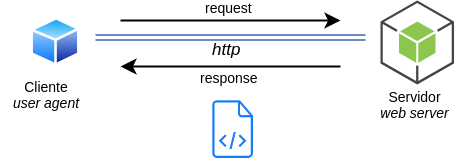
\includegraphics[width=0.9\textwidth]{img/chapter03/ui-web-arquitectura.png}
	\caption[Diagrama de una arquitectura cliente - servidor]{Diagrama de una arquitectura cliente - servidor. \textit{Fuente: ~\cite{uqbar-wiki-web}}}
	\label{fig:cliente-servidor}  % Etiqueta para la figura
\end{figure}qu


\begin{itemize}	
	\item \textbf{Arquitectura del lado del cliente:} El script del lado del cliente se encarga de gestionar la funcionalidad de la interfaz de usuario, que incluye elementos como botones y menús desplegables. Cuando el usuario final accede a la aplicación web mediante un enlace, el navegador carga el script del lado del cliente y renderiza tanto los elementos visuales como el texto necesario para la interacción con el usuario. Por ejemplo, el usuario puede visualizar contenidos, reproducir videos o completar la información de un formulario de contacto. Acciones como hacer clic en el botón de enviar se envían al servidor como solicitudes del cliente.
	
	\item \textbf{Arquitectura del lado del servidor:} El script del lado del servidor se encarga del procesamiento de la información. Este servidor gestiona las solicitudes realizadas por el cliente y devuelve una respuesta. Estas solicitudes pueden incluir acciones como la obtención de datos adicionales, la edición de datos o el almacenamiento de nuevos datos. Por ejemplo, si el usuario hace clic en un botón de “Leer más”, el servidor le envía contenido adicional. Si hace clic en “Enviar”, el servidor guarda los datos del usuario en una base de datos. En ciertos casos, el servidor completa la solicitud generando y enviando una página HTML completa al cliente, lo cual se denomina renderizado del lado del servidor.
\end{itemize}


\subsection{Frontend}


\subsubsection{HTML}
HTML son las siglas en inglés de lenguaje de etiquetas de hipertexto (HyperText Markup Language) es el lenguaje estándar fundamental para estructurar y presentar contenido en la web, siendo la base sobre la cual se construyen todas las páginas web. Su función principal es organizar el contenido de manera semántica, lo que significa que emplea etiquetas específicas para definir la estructura de los distintos elementos, como encabezados, párrafos, listas, imágenes y enlaces, permitiendo que los navegadores interpreten y muestren adecuadamente el contenido al usuario. Esta estructuración semántica facilita la accesibilidad, ya que herramientas de asistencia, como los lectores de pantalla, pueden entender y transmitir mejor la información a personas con discapacidades visuales o cognitivas, y además optimiza el SEO (Search Engine Optimization), ayudando a los motores de búsqueda a indexar y clasificar el contenido de manera más precisa y efectiva. ~\cite{HTMLMDN}

\subsubsection{CSS}
CSS son las siglas en inglés de hojas de estilo en cascada (Cascading Style Sheets) es básicamente un lenguaje que maneja el diseño y presentación de una aplicación web, es decir, cómo lucen cuando un usuario las visita. Funciona junto con el lenguaje HTML que se encarga del contenido básico de los sitios. Se les denomina hojas de estilo “en cascada” porque se puede tener varias y una de ellas con las propiedades heredadas (o en cascada) de otras.
En general, una plantilla básica resulta suficiente para el funcionamiento de una aplicación web. Sin embargo, si se desea dar una apariencia llamativa para el usuario, se necesita implementar CSS yq eu ayudará a maximizar el impacto del contenido del sitio ~\cite{CSSMDN}.  

\subsection{Backend}

\subsubsection{JavaScript}
JavaScript es un lenguaje de programación que permite brindar interactividad a las aplicaciones web. Desde actualizar fuentes de redes sociales a mostrar animaciones y mapas interactivos, las funciones de JavaScript pueden mejorar la experiencia del usuario de un sitio web. Como lenguaje de scripting del lado del servidor, se trata de una de las principales tecnologías de la World Wide Web. Por ejemplo, al navegar por Internet, en cualquier momento en el que vea un carrusel de imágenes, un menú desplegable “click-to-show” (clic para mostrar), o cambien de manera dinámica los elementos de color en una página web, estará viendo los efectos de JavaScript ~\cite{JavascriptMDN}.



\subsection{NodeJS}
Node.js es un entorno de ejecución de un solo hilo, de código abierto y multiplataforma diseñado para desarrollar aplicaciones de red y del lado del servidor rápidas y escalables de JavaScript (de ahí su terminación en .js haciendo alusión al lenguaje JavaScript). Está escrito en C/C++ y Javascript y emplea una arquitectura de E/S basada en eventos y sin bloqueos, lo que la vuelve eficaz y apropiada para aplicaciones en tiempo real ~\cite{NodeJSKinsta}. 

\begin{figure}[H]
	\centering
	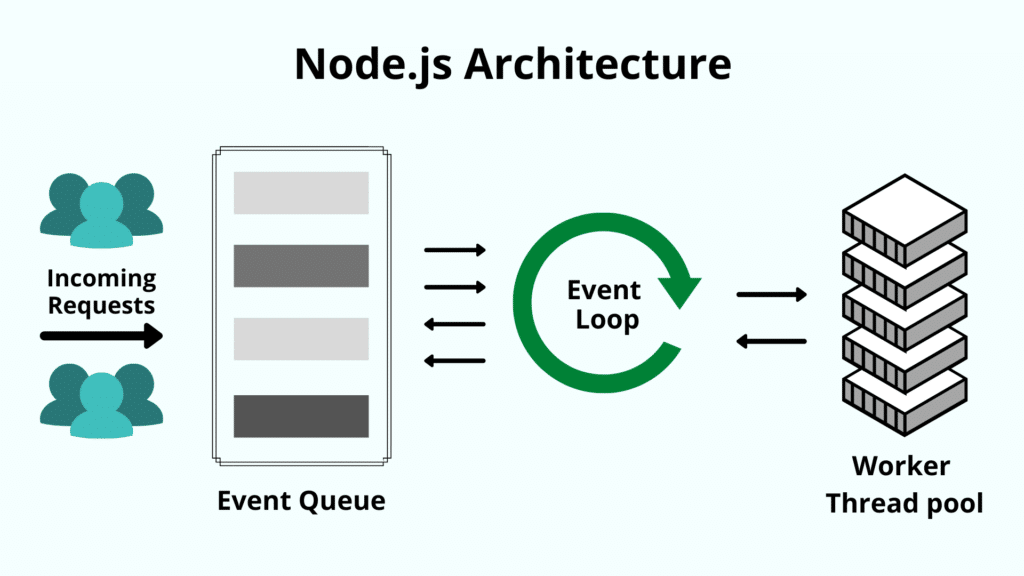
\includegraphics[width=0.8\textwidth]{img/chapter03/node-architecture.png}
	\caption[Cómo procesa node.js las peticiones entrantes utilizando el bucle de eventos]{Cómo procesa node.js las peticiones entrantes utilizando el bucle de eventos. \textit{Fuente: ~\cite{NodeJSKinsta}}}
	\label{fig:nodejs_arqui}  % Etiqueta para la figura
\end{figure}
Node.js utiliza una arquitectura de “Single Threaded Event Loop” \ref{fig:nodejs_arqui} que maneja múltiples solicitudes mediante un único bucle de eventos y un pool de hilos limitado para operaciones de E/S bloqueantes. A diferencia del modelo multihilo de lenguajes como Java, donde cada solicitud se asigna a un hilo individual del pool, Node.js coloca las solicitudes entrantes en una cola y las procesa de manera no bloqueante, asignando hilos del pool de trabajadores solo cuando es necesario. Esta arquitectura reduce el consumo de recursos y memoria, permitiendo una ejecución más rápida de tareas ligeras y haciendo que Node.js sea ideal para aplicaciones en tiempo real. Sin embargo, para tareas que requieren un procesamiento intensivo de datos, los lenguajes multihilo como Java son más adecuados ~\cite{NodeJSKinsta}.

 
%\subsubsection{Introducción a NodeJS}
%Explicación básica sobre NodeJS.
%\subsubsection{Ventajas del uso de NodeJS para aplicaciones web}
%Descripción de por qué se eligió NodeJS para la parte del servidor.
%\subsubsection{Integración de NodeJS con Maxima}
%Detalle de cómo se usa NodeJS para comunicarse con Maxima y realizar cálculos matemáticos.

\subsection{Maxima}
Maxima es un Sistema de Álgebra Computacional (CAS, por sus siglas en inglés: Computer Algebra System) diseñado en Lisp, de código abierto diseñado para realizar manipulaciones simbólicas y numéricas de expresiones matemáticas. Originalmente desarrollado a partir de una versión de Macsyma del MIT en 1982, Maxima ha evolucionado gracias a la contribución de una comunidad de desarrolladores y usuarios que continúan mejorándolo y ampliando sus capacidades ~\cite{MaximaSourgeforce}.  \newline
Se destaca por ser muy rápido y ligero, lo que permite realizar manipulaciones simbólicas y numéricas de manera eficiente, incluyendo simplificación, derivadas, integrales y resolución de ecuaciones algebraicas y diferenciales. Además, maneja operaciones avanzadas con matrices y vectores, genera gráficos bidimensionales y tridimensionales, y ofrece un lenguaje de programación propio para automatizar cálculos y crear scripts personalizados ~\cite{MaximaSourgeforce}. 
%\subsubsection{Qué es Maxima y por qué se usa para cálculos simbólicos}
%Explicación sobre el software Maxima y su importancia en los cálculos de Series de Fourier. 
%\subsubsection{Implementación de Maxima en el servidor}
%Cómo se utiliza Maxima en el servidor junto con NodeJS para realizar cálculos matemáticos de forma eficiente.

\subsection{Angular}
Angular es un Framework de JavaScript de código abierto escrito en TypeScript. Su objetivo principal es desarrollar aplicaciones de una sola página. Google se encarga del mantenimiento y constantes actualizaciones de mejoras para este framework.
En el ámbito del desarrollo de software, un framework se define como una estructura de soporte tanto conceptual como tecnológica, compuesta generalmente por artefactos o módulos de software específicos. Estos componentes sirven como base para la organización y creación de aplicaciones.
En otras palabras, un framework actúa como una plantilla o esquema fundamentado en tecnología que simplifica significativamente el trabajo. De este modo, se minimizan los posibles errores de programación.
Así, un framework es un conjunto de herramientas y módulos reutilizables para distintos proyectos, lo que facilita el desarrollo en diversos aspectos, mejorando el tiempo de ejecución, el esfuerzo requerido y la organización general del proceso.

\subsubsection{TypeScript}
TypeScript es un superset de JavaScript que añade tipado estático y características avanzadas al lenguaje de programación. Desarrollado por Microsoft, TypeScript se compila a JavaScript, lo que permite utilizar sus funcionalidades en cualquier entorno que soporte JavaScript. Al incorporar tipos estáticos, TypeScript facilita la detección temprana de errores durante el desarrollo, mejora la legibilidad del código y facilita el mantenimiento de proyectos a gran escala. Además, ofrece soporte para programación orientada a objetos y otras mejoras que potencian la productividad y la robustez de las aplicaciones web. Gracias a estas ventajas, TypeScript se ha convertido en una herramienta popular en el desarrollo de aplicaciones modernas, complementando y extendiendo las capacidades de JavaScript ~\cite{TypescriptDOCS}.


\subsubsection{Tailwind CSS}
Tailwind CSS es un framework de CSS  que permite a construir interfaces de usuario personalizadas de manera rápida y eficiente. A diferencia de los frameworks tradicionales que proporcionan componentes predefinidos, Tailwind ofrece clases de utilidad que pueden combinarse directamente en el HTML sin necesidad de escribir CSS personalizado. Esto facilita la creación de diseños responsivos y altamente personalizables, promoviendo la consistencia y reduciendo la cantidad de código CSS necesario. Además, Tailwind incluye características como el modo oscuro, diseños flexibles y un sistema de personalización extensivo que permite adaptar el framework a las necesidades específicas de cada proyecto~\cite{TailwindCSS}.

\subsection{API}
Una API, por sus siglas en ingles de interfaz de programación de aplicaciones (application programming interface), es un conjunto de definiciones y protocolos que se utiliza para desarrollar e integrar los sistemas de software de las aplicaciones. Al compartir únicamente la información necesaria y ocultar detalles internos, las API mejoran la seguridad del sistema ~\cite{APIDazzet}. 
\begin{figure}[H]
	\centering
	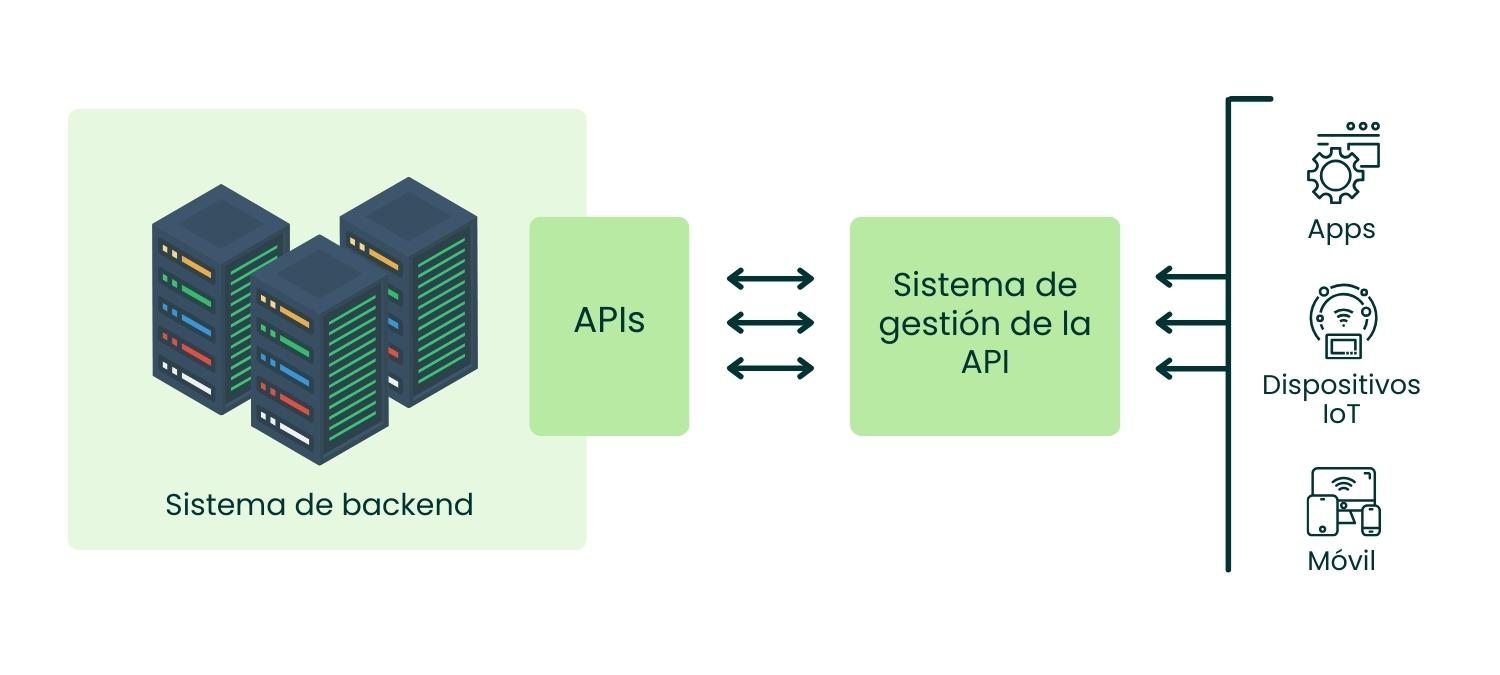
\includegraphics[width=0.8\textwidth]{img/chapter03/API-architecture.jpg}
	\caption[Arquitectura general de una API.]{Arquitectura general de una API.\textit{Fuente: ~\cite{APIDazzet}}}
	\label{fig:api_arqui}  % Etiqueta para la figura
\end{figure}
Suele considerarse como el contrato entre el usuario y el  proveedor de información, en el cual se establece el contenido que se necesita por parte del consumidor (la llamada) y el que requiere el productor (la respuesta). Se puede considerar la API como el mediador entre los usuarios o clientes y los recursos o servicios web que quieren obtener. Con ellas, las empresas pueden compartir recursos e información mientras conservan la seguridad, el control y la autenticación, lo cual les permite definir los accesos de cada usuario~\cite{APIDazzet}. 

\subsubsection{Protocolo HTTP}
El HTTP, que viene de las siglas en inglés de Protocolo de Transferencia de Hiper Texto (HyperText Transfer Protocol) es el protocolo esencial para la transmisión de información en la World Wide Web, facilitando la comunicación entre servidores, clientes y proxies mediante un lenguaje común. Establecido en 1999 por el World Wide Web Consortium y la Internet Engineering Task Force, define las reglas de sintaxis y semántica para las peticiones y respuestas, operando principalmente a través de los puertos 80 y 8080. Al ser un protocolo sin estado, no guarda registro de interacciones anteriores, pero utiliza cookies para almacenar información de visitas previas en el cliente. Su funcionamiento se basa en un esquema de petición-respuesta, permitiendo una comunicación eficiente y flexible entre el usuario (como navegadores o rastreadores web) y los servidores web ~\cite{HTTPEditorialEtece}.

\subsubsection{REST}
REST significa Representational State Transfer, este no es un protocolo ni un estándar, sino un conjunto de restricciones vinculadas a la arquitectura. REST define un conjunto de funciones como GET, PUT, DELETE, etc. que los clientes pueden usar para acceder a los datos del servidor. Los clientes y servidores intercambian datos utilizando el protocolo HTTP.

La característica principal de las API REST es la falta de estado (statelessness). Esto significa que los servidores no guardan los datos del cliente entre las solicitudes. Las solicitudes del cliente al servidor son similares a las URL que escribes en tu navegador para visitar un sitio web. La respuesta del servidor es solo datos en formato plano, sin la representación gráfica típica de una página web~\cite{APIDazzet}.

\subsection{Interfaz gráfica de usuario}
Las Interfaces Gráficas de Usuario (GUI) son omnipresentes en nuestra vida cotidiana, ya sea al utilizar una computadora o un celular entre otros dispositivos. La eficacia de una GUI es crucial para determinar si un producto será competitivo o no. Un producto puede fracasar si el usuario no logra completar una acción, como una transacción económica, si no comprende la secuencia de pasos requeridos, si no encuentra fácilmente cómo realizar una acción necesaria, como hacer una compra, o si no encuentra atractivo el diseño de la aplicación. ~\cite{interfazAlbornoz}
\subsubsection{Principios de Usabilidad}
Los principios de usabilidad web son la base de cualquier página web para que sea “user friendly”. O lo que es lo mismo, es un tipo de diseño centrado en el usuario para conseguir mejorar la experiencia del mismo. La usabilidad se refiere a la facilidad con la que los usuarios interactúan con una herramienta con el fin de lograr un propósito específico. Así pues, la usabilidad web indica hasta qué punto un sitio web resulta sencillo de utilizar. Esto significa que para que una apliación web ~\cite{usabilidadJakob}. \newline
Los principios de usabilidad, son diez fundamentos que facilitan el diseño de productos más aceptados por los usuarios al enfocarse en sus necesidades y comportamientos~\cite{usabilidadJakob}:
\begin{enumerate}
	\item \textbf{Visibilidad del estado del sistema.} El usuario siempre debe de estar informado de lo que está pasando en en la aplicación web y ofrecerle una respuesta en el menor tiempo posible. Ejemplos de esto son las barras de carga o notificaciones sobre el navegador.
	
	\item \textbf{Relación entre el sistema y el mundo real.} El sistema tiene que “hablar” el lenguaje del usuario usando palabras, frases inclusive símbolos con los que el esté familiarizado y que pueda reconocer con facilidad. Para esto la información debe mostrarse en un orden lógico y usando las palabras y símbolos correctos, sin darle oportunidad al usuario de equivocarse.
	\item \textbf{Control y libertad del usuario.} Los usuarios pueden equivocarse al realizar una acción dentro de la apliación, así que este debe tener la oportunidad de corregir su error y no sentirse frustrado por ello. Claro ejemplo de esto es un botón de deshacer.
	
	\item \textbf{Consistencia y estándares.} Las aplicaciones deben de seguir los estándares y convenios establecidos para iconos o colores, por ejemplo un icono con lineas verticales indica un menú, o el color verde y rojo se asocian con aceptar y cancelar, respectivamente.
	
	\item \textbf{Prevención de errores.} La apliación debe de prevenir cualquier posible error que el usuario pueda cometer, y encaso de que este cometa uno, debe de disponer de diversas herramientas para corregirlo, limitar caracteres o entradas no validas por el sistema es un ejemplo de esto.
	
	\item \textbf{Reconocer antes que recordar.} La apliación debe ayudar al usuario a no tener que memorizar acciones u objetos para que pueda usarla fácilmente, usar botones asignados y personalizados para acciones especificas es un ejemplo de esto.
	 
	\item \textbf{Flexibilidad y eficiencia de uso.} La apliación debe de de estar preparada para recibir a todo tipo de usuarios, si alguien inexperto en el sitio o en el tema del mismo se pueden brindar ayudas como ventanas con mensajes o tutoriales. 
	
	\item \textbf{Diseño estético y minimalista.} La apliación no debe de tener información innecesaria que distraiga al usuario y perturbe su experiencia al usarla.
	
	\item \textbf{Ayudar a los usuarios a reconocer, diagnosticar y corregir los errores.} En caso de que se produzca un error o excepción dentro de la aplicación, los mensajes de error deben ser compresibles para el usuario, como pasar de un ERROR 404 a un mensaje mas entendible como ERROR DEL SERVIDOR.
	
	\item \textbf{Ayuda y documentación.} Es preciso que la apliación cuente con un manual de funcionamiento, esto ayuda al usuario a que le sea mas fácil usar la apliación. Este manual debe ser facil de localizar, definir los pasos claramente y no de manera extensa.
\end{enumerate}

El cumplir con estos principios de usabilidad ayudan a que el sitio cuente con un trafico más recurrente, es decir, aumentamos las posibilidades de que un usuario, después de utilizar la apliación, la vuelva a usar en un futuro, así como que más personas la usen, demás de que se disminuye el porcentaje de rebote, que no es otra cosa que conseguir que el tiempo de estancia del usuario en la aplicación sea más alto y que explore mas partes del sitio.


\subsection{Seguridad en Aplicaciones Web}
La seguridad en aplicaciones web es fundamental para proteger la integridad, confidencialidad y disponibilidad de los datos manejados, así como para garantizar la confianza de los usuarios. Algunas medidas que se implementan en una aplicación web para implementar dicha seguridad son las siguientes.

\subsubsection{Protocolo HTTPS}
El protocolo de transferencia de hipertexto seguro, por sus siglas en inglés, (HyperText Transfer Protocol Secure) es una versión segura del protocolo HTTP que utiliza el SSL\slash TLS para cifrado y autenticación. HTTPS está especificado por RFC 2818~\cite{RFC2818} y utiliza el puerto 443 o el 8443 de forma predeterminada en lugar del puerto 80/8080 de HTTP ~\cite{HTTPS-SSL}. \newline
El protocolo HTTPS hace posible que los usuarios del sitio web transmitan datos confidenciales como números de tarjetas de crédito, información bancaria y credenciales de inicio de sesión de forma segura a través de Internet. Por esta razón, HTTPS es especialmente importante para asegurar actividades en línea como compras, banca y trabajo remoto. Sin embargo, HTTPS se está convirtiendo rápidamente en el protocolo estándar para cualquier sitio web, ya sea que este intercambie o no datos confidenciales con los usuarios ~\cite{HTTPS-SSL}.\newline
HTTPS se diferencia de HTTP al agregar cifrado, autenticación e integridad al protocolo original. Mediante SSL/TLS, HTTPS cifra los datos para protegerlos de interceptaciones y ataques de intermediarios, utilizando criptografía de clave pública para establecer una conexión segura entre el servidor y el navegador. Además, HTTPS autentica la identidad del servidor mediante certificados digitales emitidos por autoridades de certificación confiables, garantizando que los documentos provienen de una fuente legítima. También asegura la integridad de los datos mediante firmas digitales que verifican que el contenido no ha sido alterado durante la transmisión. Estas mejoras hacen que HTTPS sea un protocolo mucho más seguro para navegar y realizar transacciones en la web en comparación con HTTP ~\cite{HTTPS-SSL}.

\subsubsection{Certificado SSL/TLS}
El certificado SSL (Secure Sockets Layer) es una pieza clave para establecer una conexión segura entre el servidor y el cliente. Este establece un enlace cifrado entre un servidor y un cliente. Esto permite que información confidencial, como los datos de la tarjeta de crédito, se transmita de forma segura a través de Internet.El certificado contiene una clave pública que autentica la identidad del sitio web y permite la transferencia de datos cifrados mediante criptografía asimétrica o de clave pública. La clave privada correspondiente se mantiene en secreto en el servidor ~\cite{SSL-TLS}.

\subsection{Graficos y visualización de datos}
\subsubsection{Canvas}
El elemento \texttt{<canvas>} en HTML es una herramienta que permite dibujar gráficos, crear animaciones y renderizar imágenes en tiempo real a través de scripting. El elemento \texttt{<canvas>} es sólo un contenedor de gráficos. Es necesario usar JavaScript para crear los gráficos. Canvas cuenta con varios métodos para dibujar trazados, cuadros, círculos, texto así como agregar imágenes. Canvas también es compatible con todos los principales navegadores ~\cite{CanvasHTMLW3S}.  s
%
%
%\section{Recommendations and future work}
%\begin{table}[hbtp]
%	\centering
%	\begin{tabular}{@{}*{2}{p{0.5\textwidth}}@{}}
%		\toprule
%		\textbf{Correct} &  \textbf{Incorrect}
%		\\
%		\midrule
%		\enquote{This is an \enquote{inner quote} inside an outer quote}
%		&
%		"This is an 'inner quote' inside an outer quote"
%		\\
%		\bottomrule
%	\end{tabular}
%	\caption[Quotation marks]
%	{Proper quotation mark usage.
%		The \texttt{\textbackslash enquote} command chooses the correct
%		quotation marks for the specified language.}
%\end{table}
%\lipsum[1]
	\chapter{Análisis del sistema}\label{ch:Análisis y diseño del sistema}
En este capítulo se evaluaron los datos del marco teórico para seleccionar los componentes más adecuados para el proyecto. También se realizó un análisis detallado de los requerimientos y riesgos asociados al desarrollo del sistema, asegurando un diseño eficiente y viable para su implementación.

\section{Metodología de Desarrollo}
La metodología a usar	La metodología propuesta para el desarrollo del proyecto es Prototipos Evolutivos, en la cual se emplearán dos iteraciones mínimas. Esta metodología es adecuada para proyectos en los que la comprensión completa de los requisitos puede surgir gradualmente y en donde es importante recibir retroalimentación continua ~\cite{MetodologíasDeDesarrollo2015}. Al utilizar prototipos, se permite una aproximación más ágil al desarrollo, ya que se pueden generar soluciones tempranas que serán ajustadas en función de los comentarios de los usuarios y evaluaciones constantes.

\begin{figure}[H]
	\centering
	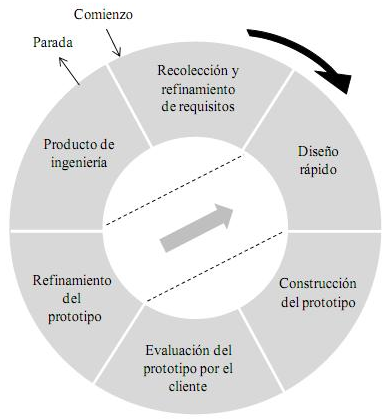
\includegraphics[width=0.5\textwidth]{img/chapter04/prototipo.png}
	\caption[Etapas de la metodología por prototipos.]{tapas de la metodología por prototipos. \textit{Fuente: ~\cite{MetodologíasDeDesarrollo2015}}}
	\label{fig:prototpios-metodología}  % Etiqueta para la figura
\end{figure}

El uso de prototipos permite abordar los requerimientos del sistema de manera iterativa. Cada prototipo no es desechado sino que se mejora progresivamente hasta obtener una versión completa del sistema. Esto asegura que el producto final no solo cumpla con los requisitos establecidos inicialmente, sino también con las expectativas del cliente o usuario. \newline 
La retroalimentación temprana que se recibe desde las primeras etapas del proyecto es invaluable para identificar mejoras y posibles problemas antes de que se conviertan en obstáculos mayores. Esto permite un ahorro significativo de tiempo y recursos, ya que se pueden realizar correcciones antes de que los problemas se propaguen en el ciclo de desarrollo. Algunas de las principales ventajas de usar esta metodología son: \newline 
\begin{itemize}
	\item Permite obtener retroalimentación temprana y frecuente del cliente, lo que ayuda a ajustar los requerimientos de manera rápida.
	\item Facilita la detección temprana de errores o problemas de diseño, lo que reduce costos de desarrollo en fases posteriores.
	\item Mejora la comprensión de los requisitos por parte del equipo de desarrollo y el cliente, reduciendo malentendidos.
	\item Aumenta la satisfacción del cliente al ver un producto tangible en las primeras fases del desarrollo.
	\item Fomenta la iteración y mejora continua del producto, asegurando que se ajuste mejor a las necesidades reales del cliente.
\end{itemize}


\section{Análisis de Requerimientos}
El análisis de requerimientos tiene la finalidad de establecer las bases del proyecto, ya que permiten conocer si realmente se está entendiendo la problemática principal que se está tratando para garantizar que la solución propuesta es ideal para dar una solución fiable. 
Con esto en mente, partimos de los resultados de la encuesta y la investigación realizada en el estado del arte \ref{ch:Estado del Arte}, se han considerado los requerimientos que se detallan a continuación.
\subsection{Requerimientos Funcionales}
Los requerimientos funcionales describen lo que el sistema debe hacer, es decir, las funcionalidades o tareas específicas que debe realizar para cumplir su propósito. A continuación, se muestran en las siguientes tablas los requerimientos funcionales para el desarrollo del sistema cuyo proposito es calcular y graficar series de Fourier.

% Requerimiento 1
\begin{longtable}{|m{3.5cm}|m{9.5cm}|}
	\hline
	\rowcolor{black!75} \color{white}\textbf{Requerimiento} & \color{white}\textbf{Entrada para la función $f$} \\
	\hline
	\endfirsthead
	\multicolumn{2}{c}{{\tablename\ \thetable{} -- continuación}} \\
	\hline
	\rowcolor{black!75} \color{white}\textbf{Requerimiento} & \color{white}\textbf{Entrada para la función $f$} \\
	\hline
	\endhead
	\hline \multicolumn{2}{r}{{Continúa en la siguiente página}} \\
	\endfoot
	\hline
	\endlastfoot
	
	\textbf{Identificador} & RF1 \\
	\hline
	\textbf{Prioridad de desarrollo} & Alta \\
	\hline
	\textbf{Entrada} & Función \( f \) ingresada por el usuario, ya sea en términos de $x$ o de $t$, en formato de notación matemática, como una sola función o como una función a trozos incluyendo los intervalos de \(t\) o $x$. \\
	\hline
	\textbf{Salida} & Captura y representación de la función ingresada en notación matemática en la interfaz. \\
	\hline
	\textbf{Descripción} & El sistema permitirá al usuario ingresar una función \( f \), en un campo de entrada fácil de entender. Proporcionar botones de añadir (\scalebox{0.8}{\faIcon{plus-circle}}) y quitar (\scalebox{0.8}{\faIcon{minus-circle}}) para agregar o eliminar trozos de la función sin necesidad de preguntar explícitamente si es una función a trozos. \\
	\hline
	\textbf{Precondición} & El usuario debe estar en la interfaz de entrada de función. \\
	\hline
	\textbf{Postcondición} & La función ingresada se mostrará en notación matemática y estará lista para validación y procesamiento. \\
	\hline
\end{longtable}
\caption{Requerimiento funcional No. 1} \label{tabla:RF1}
\vspace{0.5cm}

% Requerimiento 2
\begin{longtable}{|m{3.5cm}|m{9.5cm}|}
	\hline
	\rowcolor{black!75} \color{white}\textbf{Requerimiento} & \color{white}\textbf{Teclado en pantalla para entrada de funciones} \\
	\hline
	\endfirsthead
	\multicolumn{2}{c}{{\tablename\ \thetable{} -- continuación}} \\
	\hline
	\rowcolor{black!75} \color{white}\textbf{Requerimiento} & \color{white}\textbf{Teclado en pantalla para entrada de funciones} \\
	\hline
	\endhead
	\hline \multicolumn{2}{r}{{Continúa en la siguiente página}} \\
	\endfoot
	\hline
	\endlastfoot
	
	\textbf{Identificador} & RF2 \\
	\hline
	\textbf{Prioridad de desarrollo} & Media \\
	\hline
	\textbf{Entrada} & Interacción del usuario con el teclado en pantalla para ingresar funciones y símbolos matemáticos como $sin()$, $cos()$, $sinh()$, $cosh()$, $exp()$, exponentes y fracciones. \\
	\hline
	\textbf{Salida} & Función correctamente ingresada en notación matemática en la interfaz de usuario, utilizando los símbolos seleccionados del teclado en pantalla. \\
	\hline
	\textbf{Descripción} & La interfaz debe mostrar un teclado en pantalla que incluya funciones matemáticas y símbolos comunes, tales como funciones trigonométricas ($sin()$, $cos()$), hiperbólicas ($cos()$, $sinh()$), exponenciales ($exp()$), operaciones de potencia y fracciones. Esto permitirá al usuario ingresar funciones de manera precisa y eficiente. \\
	\hline
	\textbf{Precondición} & El usuario debe tener acceso a la interfaz de entrada de funciones con el teclado en pantalla activado. \\
	\hline
	\textbf{Postcondición} & La función ingresada aparece en el campo de entrada en notación matemática, lista para su procesamiento. \\
	\hline
\end{longtable}
\captionof{table}{Requerimiento funcional No. 2} \label{tabla:RF2}
\vspace{0.5cm}

% Requerimiento 3
\begin{longtable}{|m{3.5cm}|m{9.5cm}|}
	\hline
	\rowcolor{black!75} \color{white}\textbf{Requerimiento} & \color{white}\textbf{Selección del tipo de serie de Fourier} \\
	\hline
	\endfirsthead
	\multicolumn{2}{c}{{\tablename\ \thetable{} -- continuación}} \\
	\hline
	\rowcolor{black!75} \color{white}\textbf{Requerimiento} & \color{white}\textbf{Selección del tipo de serie de Fourier} \\
	\hline
	\endhead
	\hline \multicolumn{2}{r}{{Continúa en la siguiente página}} \\
	\endfoot
	\hline
	\endlastfoot
	
	\textbf{Identificador} & RF3 \\
	\hline
	\textbf{Prioridad de desarrollo} & Media \\
	\hline
	\textbf{Entrada} & El usuario selecciona el tipo de serie a utilizar entre opciones de serie trigonométrica o serie exponencial compleja. Si selecciona la serie trigonométrica, puede optar por extensiones periódicas de rango completo o de medio rango (extensión par usando serie de cosenos o extensión impar usando serie de senos). \\
	\hline
	\textbf{Salida} & El tipo de serie y extensión seleccionados quedan registrados y configurados en la interfaz, listos para el cálculo de la serie correspondiente. \\
	\hline
	\textbf{Descripción} & El sistema permite al usuario seleccionar entre opciones de series de Fourier: serie trigonométrica o serie exponencial compleja. Para la serie trigonométrica, el usuario puede elegir entre una extensión periódica de rango completo (opción por defecto) o una extensión de medio rango (par o impar), con la condición de que la función comience en \( t = 0 \) para las extensiones de medio rango. Si para estas no se selecciona una extensión impar o par, automáticamente se tomará la extensión periódica que incluye senos y cosenos. \\
	\hline
	\textbf{Precondición} & El usuario debe estar en la interfaz de selección de series de Fourier y tener una función cargada para análisis de serie. \\
	\hline
	\textbf{Postcondición} & El tipo de serie y la extensión seleccionada quedan configurados y visibles en la interfaz para su validación y procesamiento. \\
	\hline
\end{longtable}
\caption{Requerimiento funcional No. 3} \label{tabla:RF3}
\vspace{0.5cm}

% Requerimiento 4
\begin{longtable}{|m{3.5cm}|m{9.5cm}|}
	\hline
	\rowcolor{black!75} \color{white}\textbf{Requerimiento} & \color{white}\textbf{Validación de funciones compatibles} \\
	\hline
	\endfirsthead
	\multicolumn{2}{c}{{\tablename\ \thetable{} -- continuación}} \\
	\hline
	\rowcolor{black!75} \color{white}\textbf{Requerimiento} & \color{white}\textbf{Validación de funciones compatibles} \\
	\hline
	\endhead
	\hline \multicolumn{2}{r}{{Continúa en la siguiente página}} \\
	\endfoot
	\hline
	\endlastfoot
	
	\textbf{Identificador} & RF4 \\
	\hline
	\textbf{Prioridad de desarrollo} & Alta \\
	\hline
	\textbf{Entrada} & Función ingresada por el usuario en el campo de entrada de funciones. \\
	\hline
	\textbf{Salida} & Mensaje de notificación en la interfaz si la función ingresada es inválida para el cálculo de la Serie de Fourier. \\
	\hline
	\textbf{Descripción} & El sistema debe contar con un catálogo de funciones no válidas para el cálculo de Series de Fourier, (como \( \ln(t) \), $csc(t)$). Si el usuario ingresa una función inválida, el sistema debe informarle y evitar el proceso de cálculo, asegurando que solo funciones compatibles continúen al procesamiento. \\
	\hline
	\textbf{Precondición} & El usuario ha ingresado una función para la validación previa al cálculo de la Serie de Fourier. \\
	\hline
	\textbf{Postcondición} & La función es verificada y, en caso de ser inválida, el sistema notifica al usuario y bloquea el cálculo de la Serie de Fourier para dicha función. \\
	\hline
\end{longtable}
\caption{Requerimiento funcional No. 4} \label{tabla:RF4}
\vspace{0.5cm}


% Requerimiento 5
\begin{longtable}{|m{3.5cm}|m{9.5cm}|}
	\hline
	\rowcolor{black!75} \color{white}\textbf{Requerimiento} & \color{white}\textbf{Parseo de entrada de funciones para procesamiento.} \\
	\hline
	\endfirsthead
	\multicolumn{2}{c}{{\tablename\ \thetable{} -- continuación}} \\
	\hline
	\rowcolor{black!75} \color{white}\textbf{Requerimiento} & \color{white}\textbf{Parseo de entrada de funciones para procesamiento} \\
	\hline
	\endhead
	\hline \multicolumn{2}{r}{{Continúa en la siguiente página}} \\
	\endfoot
	\hline
	\endlastfoot
	
	\textbf{Identificador} & RF5 \\
	\hline
	\textbf{Prioridad de desarrollo} & Alta \\
	\hline
	\textbf{Entrada} & Expresión matemática ingresada por el usuario en formato de notación matemática (\LaTeX). \\
	\hline
	\textbf{Salida} & Expresión convertida a un formato compatible para procesamiento matemático en el backend, enviada mediante una solicitud en formato JSON. \\
	\hline
	\textbf{Descripción} & El sistema debe interpretar y convertir las entradas matemáticas en notación \LaTeX~ a un formato compatible con el motor de cálculo. Los datos convertidos se envían al backend a través de una solicitud para su procesamiento. \\
	\hline
	\textbf{Precondición} & El usuario ha ingresado una expresión matemática en la interfaz. \\
	\hline
	\textbf{Postcondición} & La expresión se encuentra en el backend en un formato adecuado para su procesamiento y evaluación matemática. \\
	\hline
\end{longtable}
\caption{Requerimiento funcional No. 5} \label{tabla:RF5}
\vspace{0.5cm}

% Requerimiento 6
\begin{longtable}{|m{3.5cm}|m{9.5cm}|}
	\hline
	\rowcolor{black!75} \color{white}\textbf{Requerimiento} & \color{white}\textbf{Cálculo de coeficientes y expansión de la Serie de Fourier} \\
	\hline
	\endfirsthead
	\multicolumn{2}{c}{{\tablename\ \thetable{} -- continuación}} \\
	\hline
	\rowcolor{black!75} \color{white}\textbf{Requerimiento} & \color{white}\textbf{Cálculo de coeficientes y expansión de la Serie de Fourier} \\
	\hline
	\endhead
	\hline \multicolumn{2}{r}{{Continúa en la siguiente página}} \\
	\endfoot
	\hline
	\endlastfoot
	
	\textbf{Identificador} & RF6 \\
	\hline
	\textbf{Prioridad de desarrollo} & Alta \\
	\hline
	\textbf{Entrada} & Función ingresada por el usuario y configuraciones para el cálculo de la Serie de Fourier, como el número de términos deseado en la expansión. \\
	\hline
	\textbf{Salida} & Serie de Fourier generada, con los coeficientes calculados \( a_0 \), \( a_n \), \( b_n \) o \( c_n \), y expansión de la serie hasta el número especificado de términos. \\
	\hline
	\textbf{Descripción} & El sistema utiliza un motor de cálculo simbólico en el backend para resolver los integrales necesarios, calcular los coeficientes de Fourier \( a_0 \), \( a_n \), \( b_n \) o \( c_n \), y generar la expansión de la Serie de Fourier hasta 50 términos. \\
	\hline
	\textbf{Precondición} & El usuario ha ingresado una función válida y configurado los parámetros para el cálculo de la Serie de Fourier. \\
	\hline
	\textbf{Postcondición} & La Serie de Fourier calculada y sus coeficientes se encuentran disponibles en la interfaz para visualización y análisis. \\
	\hline
\end{longtable}
\caption{Requerimiento funcional No. 6} \label{tabla:RF6}
\vspace{0.5cm}

% Requerimiento 7
\begin{longtable}{|m{3.5cm}|m{9.5cm}|}
	\hline
	\rowcolor{black!75} \color{white}\textbf{Requerimiento} & \color{white}\textbf{Recuperación de resultados para visualización} \\
	\hline
	\endfirsthead
	\multicolumn{2}{c}{{\tablename\ \thetable{} -- continuación}} \\
	\hline
	\rowcolor{black!75} \color{white}\textbf{Requerimiento} & \color{white}\textbf{Recuperación de resultados para visualización} \\
	\hline
	\endhead
	\hline \multicolumn{2}{r}{{Continúa en la siguiente página}} \\
	\endfoot
	\hline
	\endlastfoot
	
	\textbf{Identificador} & RF7 \\
	\hline
	\textbf{Prioridad de desarrollo} & Media \\
	\hline
	\textbf{Entrada} & Solicitud de recuperación de resultados generados por el cálculo de la Serie de Fourier, en formato JSON. \\
	\hline
	\textbf{Salida} & Resultados del cálculo, convertidos para visualización gráfica y en formato \LaTeX~ para mostrar expresiones matemáticas en la interfaz. \\
	\hline
	\textbf{Descripción} & El sistema enviará los resultados del cálculo al frontend a través de una solicitud en formato JSON. La interfaz de usuario debe interpretar estos resultados y convertirlos a un formato adecuado para graficación y a formato \LaTeX~ para mostrar las expresiones matemáticas en notación visual. \\
	\hline
	\textbf{Precondición} & Los resultados de los cálculos de la Serie de Fourier están listos para su recuperación y visualización en el frontend. \\
	\hline
	\textbf{Postcondición} & Los resultados se muestran en la interfaz de usuario en formato gráfico y en notación matemática (\LaTeX) para una interpretación visual y análisis claros. \\
	\hline
\end{longtable}
\caption{Requerimiento funcional No. 7} \label{tabla:RF7}
\vspace{0.5cm}

% Requerimiento 8
\begin{longtable}{|m{3.5cm}|m{9.5cm}|}
	\hline
	\rowcolor{black!75} \color{white}\textbf{Requerimiento} & \color{white}\textbf{Gráfica interactiva de la función y su aproximación} \\
	\hline
	\endfirsthead
	\multicolumn{2}{c}{{\tablename\ \thetable{} -- continuación}} \\
	\hline
	\rowcolor{black!75} \color{white}\textbf{Requerimiento} & \color{white}\textbf{Gráfica interactiva de la función y su aproximación} \\
	\hline
	\endhead
	\hline \multicolumn{2}{r}{{Continúa en la siguiente página}} \\
	\endfoot
	\hline
	\endlastfoot
	
	\textbf{Identificador} & RF8 \\
	\hline
	\textbf{Prioridad de desarrollo} & Alta \\
	\hline
	\textbf{Entrada} & La función original \( f \) y su aproximación de Serie de Fourier, así como el número de términos especificado por el usuario. \\
	\hline
	\textbf{Salida} & Gráfica interactiva en la interfaz que muestra tanto la función original como su aproximación mediante Serie de Fourier. \\
	\hline
	\textbf{Descripción} & El sistema debe graficar la función original \( f \) y su aproximación mediante la Serie de Fourier en una interfaz gráfica interactiva. El usuario podrá ajustar el número de términos de la serie mediante un control deslizante, y contará con herramientas para hacer zoom, panear e interactuar en tiempo real con la gráfica. La representación gráfica debe ser eficiente y de alto rendimiento para asegurar una experiencia de usuario fluida. \\
	\hline
	\textbf{Precondición} & El usuario ha ingresado la función y solicitado la visualización gráfica de su aproximación mediante Serie de Fourier. \\
	\hline
	\textbf{Postcondición} & La gráfica interactiva de la función y su aproximación de Fourier se encuentra visible y responde a las interacciones del usuario. \\
	\hline
\end{longtable}
\caption{Requerimiento funcional No. 8} \label{tabla:RF8}
\vspace{0.5cm}

% Requerimiento 9
\begin{longtable}{|m{3.5cm}|m{9.5cm}|}
	\hline
	\rowcolor{black!75} \color{white}\textbf{Requerimiento} & \color{white}\textbf{Visualización de coeficientes y expansión de la Serie de Fourier} \\
	\hline
	\endfirsthead
	\multicolumn{2}{c}{{\tablename\ \thetable{} -- continuación}} \\
	\hline
	\rowcolor{black!75} \color{white}\textbf{Requerimiento} & \color{white}\textbf{Visualización de coeficientes y expansión de la Serie de Fourier} \\
	\hline
	\endhead
	\hline \multicolumn{2}{r}{{Continúa en la siguiente página}} \\
	\endfoot
	\hline
	\endlastfoot
	
	\textbf{Identificador} & RF9 \\
	\hline
	\textbf{Prioridad de desarrollo} & Media \\
	\hline
	\textbf{Entrada} & Coeficientes calculados \( a_0 \), \( a_n \), \( b_n \), \( c_n \), y la expresión completa de la Serie de Fourier para la función \( f(t) \). \\
	\hline
	\textbf{Salida} & Visualización clara y legible de los coeficientes calculados, la función original \( f(t) \), y la expansión de la Serie de Fourier. \\
	\hline
	\textbf{Descripción} & El sistema debe mostrar los coeficientes \( a_0 \), \( a_n \), \( b_n \) y \( c_n \), junto con la función original \( f \) y su expansión en Series de Fourier $f = \sum$. Las expresiones matemáticas deben presentarse de manera clara y legible, permitiendo al usuario comprender y revisar los cálculos y resultados de forma efectiva. \\
	\hline
	\textbf{Precondición} & Los coeficientes de la Serie de Fourier y la expansión han sido calculados y están listos para su visualización. \\
	\hline
	\textbf{Postcondición} & Las expresiones matemáticas se muestran de manera clara en la interfaz, facilitando la interpretación y revisión de los resultados por parte del usuario. \\
	\hline
\end{longtable}
\caption{Requerimiento funcional No. 9} \label{tabla:RF9}
\vspace{0.5cm}



\subsection{Requerimientos No Funcionales}
Los requerimientos funcionales definen cómo debe funcionar el sistema, además de características y restricciones que debe cumplir la aplicación, además de su funcionalidad básica.

%Tabla de no funcionales
\begin{longtable}{|m{5cm}|m{8.5cm}|}
	\hline
	\rowcolor{black!75}
	\head {Nombre} & \head {Descripción} \\ \hline
	\endfirsthead
	\multicolumn{2}{c}{{\tablename\ \thetable{} -- continuación}} \\
	\rowcolor{black!75}
	\head {Nombre} & \head {Descripción}\\ \hline
	\endhead
	\hline \multicolumn{2}{r}{{Continúa en la siguiente página}} \\
	\endfoot
	\hline
	\endlastfoot
	
	\textbf{Rendimiento} & El sistema debe ser capaz de calcular las Series de Fourier en un tiempo razonable  y devolver los resultados al usuario, asegurando fluidez en la interacción con la aplicación. La visualización de los gráficos debe ser fluida al agregar o quitar términos de la serie. \\ 
	\hline
	
	\textbf{Modularidad} & Cada microservicio debe ser autónomo, encargado de una tarea específica (por ejemplo, cálculo de series de Fourier) y desacoplado del cliente y otros microservicios, permitiendo su reemplazo o actualización sin afectar al sistema completo. \\
	\hline
		
	\textbf{Escalabilidad} & El sistema debe poder integrar nuevos microservicios en el futuro (por ejemplo, cálculo de transformadas de Fourier o análisis simbólico avanzado) sin necesidad de modificar la arquitectura base. \\ 
	\hline
	
	\textbf{Compatibilidad}  & La aplicación debe ser compatible con los principales navegadores modernos (Chrome, Firefox, Edge). A pesar de que no se definió y no es recomendable, el diseño debe ser responsivo para ajustarse a diferentes tamaños de pantalla, incluidos dispositivos móviles y tabletas. \\ \hline
	
	\textbf{Usabilidad} & La interfaz debe ser intuitiva y fácil de usar, con botones y controles claramente identificados. Los mensajes de error y advertencia deben ser comprensibles, evitando el uso de jerga técnica complicada. La notación matemática debe ser clara, precisa y visualmente agradable. \\
	\hline
	
%	\textbf{Modularidad y Extensibilidad del Código} & El frontend debe estar diseñado para facilitar la migración a frameworks como Angular en el futuro. El código debe ser modular y seguir buenas prácticas de desarrollo para facilitar la adición de nuevas características. Aunque el sistema no requiere una base de datos en su versión actual, el backend debe ser fácilmente extensible para permitir el almacenamiento de sesiones o configuraciones del usuario en el futuro. \\
%	\hline
	
	\textbf{Mantenibilidad}  & El código del sistema debe estar estructurado siguiendo buenas prácticas de desarrollo, con documentación técnica que facilite su mantenimiento y futuras mejoras. \\ \hline
	
	\textbf{Interactividad} & Las gráficas deben ser dinámicas, permitiendo zoom, desplazamiento y control del número de coeficientes de Fourier mediante un slider interactivo, con actualizaciones instantáneas. \\ \hline
	
	\textbf{Fiabilidad} & La aplicación debe manejar adecuadamente errores de entrada de funciones no válidas, mostrando mensajes claros y precisos al usuario. \\ \hline
	
	\textbf{Reusabilidad} &  El código debe estar bien documentado para que futuros desarrolladores puedan entender la lógica y estructura de la aplicación fácilmente. \\
	\hline
	
	\textbf{Seguridad} & Todas las comunicaciones entre el frontend y el backend deben estar cifradas (HTTPS). \\
	\hline
%	\textbf{Tiempo de Respuesta del Sistema} & El tiempo de respuesta del servidor para calcular coeficientes de Fourier no debe exceder los 5 segundos en condiciones normales. La gráfica debe actualizarse en menos de 500 ms para proporcionar una experiencia interactiva y sin latencia. \\
%	\hline
%	\textbf{Consumo de Recursos} & La aplicación debe ser eficiente en el uso de memoria y CPU, especialmente al realizar cálculos de series grandes. El uso de canvas debe estar optimizado para no causar retrasos en la interfaz. \\
%	\hline
%	\textbf{Compatibilidad con Carga Asíncrona} & La comunicación entre el frontend y el backend debe ser asíncrona para no bloquear la interfaz de usuario. Las llamadas a Maxima deben ser gestionadas de manera eficiente para evitar cuellos de botella. \\
%	\hline
	%\rowcolor{white} \caption{Tabla de requerimientos no funcionales} \label{tabla:RNF} \\
\end{longtable}
\caption{Tabla de requerimientos no funcionales} \label{tabla:RNF}
\vspace{0.5cm}



\section{Análisis de Riesgos}
En la gestión de proyectos, los riesgos representan cualquier evento o condición incierta que, si ocurre, puede afectar negativamente los objetivos del proyecto. Identificar y gestionar estos riesgos es crucial para minimizar su impacto y asegurar el éxito del proyecto. 
\subsection{Matriz de riesgos}
La matriz de riesgos es una herramienta clave en la gestión de proyectos, ya que permite evaluar y visualizar la gravedad y probabilidad de los riesgos que pueden afectar su éxito. Clasifica los riesgos según sus consecuencias (de "bajo" a "grave") y su frecuencia de ocurrencia (de "raro" a "casi seguro"). Al organizar estos factores en una matriz de cinco por cinco, es más fácil identificar los riesgos más críticos y priorizar las acciones correctivas. Los colores de la matriz van del verde (bajo riesgo) al rojo (alto riesgo), lo que proporciona una representación visual clara de la urgencia y el impacto de cada riesgo identificado \ref{tabla:matriz_riesgos}.

\begin{table}[H]
	\centering
	\begin{tabular}{|>{\centering\arraybackslash}m{2.5cm}|c|c|c|c|c|}
		\hline
		\rowcolor{black!75} \color{white} {\textbf{Consecuencias}} & \multicolumn{5}{c|}{ \color{white} \textbf{Probabilidad}} \\ \cline{2-6}
		\cellcolor{white} & \textbf{Casi seguro} & \textbf{Probable} & \textbf{Posible} & \textbf{Improbable} & \textbf{Raro} \\ \hline
		\textbf{Grave} & \cellcolor{red!80}Extremo & \cellcolor{red!80}Extremo & \cellcolor{red!80}Extremo & \cellcolor{orange!80}Alto & \cellcolor{yellow!60}Medio \\ \hline
		\textbf{Mayor} & \cellcolor{red!80}Extremo & \cellcolor{red!80}Extremo & \cellcolor{orange!80}Alto & \cellcolor{yellow!60}Medio & \cellcolor{yellow!60}Medio \\ \hline
		\textbf{Moderado} & \cellcolor{red!80}Extremo & \cellcolor{orange!80}Alto & \cellcolor{yellow!60}Medio & \cellcolor{yellow!60}Medio & \cellcolor{green!60}Bajo \\ \hline
		\textbf{Menor} & \cellcolor{orange!80}Alto & \cellcolor{yellow!60}Medio & \cellcolor{yellow!60}Medio & \cellcolor{green!60}Bajo & \cellcolor{green!60}Bajo \\ \hline
		\textbf{Bajo} & \cellcolor{yellow!60}Medio & \cellcolor{yellow!60}Medio & \cellcolor{green!60}Bajo & \cellcolor{green!60}Bajo & \cellcolor{green!60}Bajo \\ \hline
	\end{tabular}
	\caption[Matriz de clasificación de riesgos.]{Matriz de clasificación de riesgos. \textit{Fuente: Elaboración propia}}
	\label{tabla:matriz_riesgos}
\end{table}


\subsection{Identificación y jerarquización de riesgos}
Para poder comenzar con el análisis de riesgos pertinente, comenzamos identificación los riesgos que pueden ocurrir y, por lo tanto, afectar la correcta ejecución del proyecto, además de su jerarquización en base a su semáforo.

\begin{longtable}{|m{1.5cm}|m{4.5cm}|c|c|c|}
	\hline
	\rowcolor{black!75} \color{white} \textbf{ID Riesgo} & \color{white} \textbf{Descripción} & \color{white} \textbf{Probabilidad} & \color{white} \textbf{Impacto} & \color{white} \textbf{Semáforo} \\ 
	\hline
	\endfirsthead
	\multicolumn{5}{c}{{\tablename\ \thetable{} -- continuación}} \\
	\hline
	\rowcolor{black!75} \color{white} \textbf{ID Riesgo} & \color{white} \textbf{Descripción} & \color{white} \textbf{Probabilidad} & \color{white} \textbf{Impacto} & \color{white} \textbf{Semáforo} \\ 
	\hline
	\endhead
	\hline \multicolumn{5}{r}{{Continúa en la siguiente página}} \\
	\endfoot
	\hline
	\endlastfoot
	
	\textbf{R1} & Incapacidad temporal para continuar el proyecto debido a una enfermedad u otra causa que afecte la salud o disponibilidad. & Posible & Grave & \cellcolor{red!80} \\ 
	\hline
	\textbf{R2} & No cumplir con los objetivos del proyecto & Posible & Mayor & \cellcolor{red!80} \\ 
	\hline
	\textbf{R3} & Sobrecarga de proyectos académicos & Probable & Mayor & \cellcolor{red!80} \\ 
	\hline
	\textbf{R4} & Mala gestión del tiempo y actividades a lo largo del desarrollo del proyecto. & Posible & Mayor & \cellcolor{orange!80} \\ 
	\hline
	\textbf{R5} & Mala elección de tecnologías para el desarrollo del proyecto & Posible & Mayor & \cellcolor{orange!80} \\ 
	\hline
	\textbf{R6} & Falta de claridad o mal planteamiento de los requerimientos & Posible & Mayor & \cellcolor{orange!80} \\ 
	\hline
	\textbf{R7} & Atraso en la Entrega de Prototipos. & Posible & Mayor & \cellcolor{orange!80} \\ 
	\hline
	\textbf{R8} & Falta de conocimientos para realizar actividades relacionadas al proyecto. & Posible & Menor & \cellcolor{yellow!60} \\ 
	\hline
	\textbf{R9} & Aumento de la complejidad del proyecto. & Posible & Moderado & \cellcolor{yellow!60} \\ 
	\hline
\end{longtable}
\caption{Tabla de identificación de riesgos jerarquizada.} \label{tabla:riesgos}
\vspace{0.5cm}

Una vez se tienen identificados y jerarquizados todos los riesgos, se procede a hacer un análisis individual de cada uno.

\begin{longtable}{|m{2.5cm}|m{11cm}|}
	\hline
	\rowcolor{black!75} \multicolumn{2}{|c|}{\color{white}\textbf{Hoja de información de riesgo}} \\ 
	\hline
	\endfirsthead
	\multicolumn{2}{c}{{\tablename\ \thetable{} -- continuación}} \\
	\hline
	\rowcolor{black!75} \multicolumn{2}{|c|}{\color{white}\textbf{Hoja de información de riesgo}} \\ 
	\hline
	\endhead
	\hline \multicolumn{2}{r}{{Continúa en la siguiente página}} \\
	\endfoot
	\hline
	\endlastfoot
	
	\textbf{Riesgo ID:} & R1 \\ \hline
	\textbf{Fecha:} & 10/11/2024 \\ \hline
	\textbf{Probabilidad:} & Posible \\ \hline
	\textbf{Impacto:} & Grave \\ \hline
	\textbf{Descripción:} & Incapacidad temporal para continuar el proyecto debido a enfermedad u otra causa que afecte mi salud o disponibilidad, como único miembro del equipo. \\ \hline
	\textbf{Tipo de Riesgo:} & Rendimiento del equipo (individual). \\ \hline
	\textbf{Contexto:} & 
	\begin{itemize}
		\item \textbf{Sub-Condición 1:} Si me enfermo o enfrento una incapacidad, todo el trabajo del proyecto se detiene, ya que no hay otros miembros para continuar las actividades.
		\item \textbf{Sub-Condición 2:} La duración de la incapacidad es incierta, lo cual podría impactar significativamente el progreso del proyecto.
	\end{itemize} \\ \hline
	\textbf{Mitigación / Monitoreo:} &
	\begin{itemize}
		\item \textbf{Aceptar:} Reconocer el riesgo de interrupción en caso de incapacidad y comunicar el estado de avance a las partes interesadas regularmente.
		\item \textbf{Minimizar impacto:} Llevar un registro detallado y documentado del proyecto para que cualquier avance pueda ser retomado sin dificultades en caso de una pausa temporal.
	\end{itemize} \\ \hline
	\textbf{Plan de contingencia} & Documentar todas las actividades y avances detalladamente, manteniendo versiones de respaldo en la nube para asegurar que el proyecto pueda retomarse rápidamente tras cualquier interrupción. Informar a las partes interesadas sobre el progreso y posibles pausas debido a mi disponibilidad. \\ \hline
	\textbf{Estado Actual:} & En evaluación \\ \hline
\end{longtable}
\caption{Hoja de información de riesgo - R1} \label{tabla:R1}
\vspace{0.5cm}

\begin{longtable}{|m{2.5cm}|m{11cm}|}
	\hline
	\rowcolor{black!75} \multicolumn{2}{|c|}{\color{white}\textbf{Hoja de información de riesgo}} \\ 
	\hline
	\endfirsthead
	\multicolumn{2}{c}{{\tablename\ \thetable{} -- continuación}} \\
	\hline
	\rowcolor{black!75} \multicolumn{2}{|c|}{\color{white}\textbf{Hoja de información de riesgo}} \\ 
	\hline
	\endhead
	\hline \multicolumn{2}{r}{{Continúa en la siguiente página}} \\
	\endfoot
	\hline
	\endlastfoot
	
	\textbf{Riesgo ID:} & R2 \\ \hline
	\textbf{Fecha:} & 10/11/2024 \\ \hline
	\textbf{Probabilidad:} & Posible \\ \hline
	\textbf{Impacto:} & Mayor \\ \hline
	\textbf{Descripción:} & No cumplir con los objetivos del proyecto debido a retrasos o falta de recursos. \\ \hline
	\textbf{Tipo de Riesgo:} & Cumplimiento de objetivos. \\ \hline
	\textbf{Contexto:} & 
	\begin{itemize}
		\item \textbf{Sub-Condición 1:} Los plazos del proyecto son ajustados y cualquier retraso podría afectar el logro de los objetivos establecidos.
		\item \textbf{Sub-Condición 2:} La falta de una adecuada organización podría impedir la finalización de algunas actividades clave.
	\end{itemize} \\ \hline
	\textbf{Mitigación / Monitoreo:} &
	\begin{itemize}
		\item \textbf{Aceptar:} Aceptar el riesgo pero monitorear constantemente el avance del proyecto para detectar retrasos a tiempo.
		\item \textbf{Planificar metas intermedias:} Establecer metas de corto plazo para asegurar el progreso constante y mantener el enfoque en los objetivos principales.
	\end{itemize} \\ \hline
	\textbf{Plan de contingencia} & Revisar y ajustar el plan de trabajo regularmente para priorizar las tareas críticas. Identificar actividades que puedan ser simplificadas o pospuestas si el tiempo o los recursos se vuelven limitados. \\ \hline
	\textbf{Estado Actual:} & En fase de planificación \\ \hline
\end{longtable}
\caption{Hoja de información de riesgo - R2} \label{tabla:R2}
\vspace{0.5cm}

\begin{longtable}{|m{3cm}|m{10.5cm}|}
	\hline
	\rowcolor{black!75} \multicolumn{2}{|c|}{\color{white}\textbf{Hoja de información de riesgo}} \\ 
	\hline
	\endfirsthead
	\multicolumn{2}{c}{{\tablename\ \thetable{} -- continuación}} \\
	\hline
	\rowcolor{black!75} \multicolumn{2}{|c|}{\color{white}\textbf{Hoja de información de riesgo}} \\ 
	\hline
	\endhead
	\hline \multicolumn{2}{r}{{Continúa en la siguiente página}} \\
	\endfoot
	\hline
	\endlastfoot
	
	\textbf{Riesgo ID:} & R3 \\ \hline
	\textbf{Fecha:} & 02/03/24 \\ \hline
	\textbf{Probabilidad:} & Probable \\ \hline
	\textbf{Impacto:} & Mayor \\ \hline
	\textbf{Descripción:} & Sobrecarga de proyectos académicos que pueda limitar el tiempo dedicado al proyecto actual. \\ \hline
	\textbf{Tipo de Riesgo:} & Gestión de tiempo y recursos. \\ \hline
	\textbf{Contexto:} & 
	\begin{itemize}
		\item \textbf{Sub-Condición 1:} La carga académica en otras asignaturas o actividades podría restar tiempo al desarrollo del proyecto.
		\item \textbf{Sub-Condición 2:} Las fechas de entrega de otros proyectos coinciden con los periodos importantes de este proyecto, aumentando el riesgo de retrasos.
	\end{itemize} \\ \hline
	\textbf{Mitigación / Monitoreo:} &
	\begin{itemize}
		\item \textbf{Planificación anticipada:} Organizar un calendario de trabajo que contemple todas las responsabilidades y anticiparse a los períodos de alta carga académica.
		\item \textbf{Distribución de tareas:} Dividir el proyecto en tareas más pequeñas y alcanzables para avanzar gradualmente, incluso en semanas de alta demanda.
	\end{itemize} \\ \hline
	\textbf{Plan de contingencia} & Identificar tareas del proyecto que puedan realizarse en paralelo con otras responsabilidades académicas, aprovechando momentos libres o períodos de menor carga. De ser posible, simplificar ciertos entregables para adaptarlos a la disponibilidad de tiempo. \\ \hline
	\textbf{Estado Actual:} & En fase de planificación \\ \hline
\end{longtable}
\caption{Hoja de información de riesgo - R3} \label{tabla:R3}
\vspace{0.5cm}

\begin{longtable}{|m{3cm}|m{10.5cm}|}
	\hline
	\rowcolor{black!75} \multicolumn{2}{|c|}{\color{white}\textbf{Hoja de información de riesgo}} \\ 
	\hline
	\endfirsthead
	\multicolumn{2}{c}{{\tablename\ \thetable{} -- continuación}} \\
	\hline
	\rowcolor{black!75} \multicolumn{2}{|c|}{\color{white}\textbf{Hoja de información de riesgo}} \\ 
	\hline
	\endhead
	\hline \multicolumn{2}{r}{{Continúa en la siguiente página}} \\
	\endfoot
	\hline
	\endlastfoot
	
	\textbf{Riesgo ID:} & R4 \\ \hline
	\textbf{Fecha:} & 02/03/24 \\ \hline
	\textbf{Probabilidad:} & Posible \\ \hline
	\textbf{Impacto:} & Mayor \\ \hline
	\textbf{Descripción:} & Mala gestión del tiempo y actividades a lo largo del desarrollo del proyecto. \\ \hline
	\textbf{Tipo de Riesgo:} & Organización y planificación. \\ \hline
	\textbf{Contexto:} & 
	\begin{itemize}
		\item \textbf{Sub-Condición 1:} La falta de planificación detallada podría llevar a demoras en la ejecución de tareas críticas.
		\item \textbf{Sub-Condición 2:} La pérdida de enfoque en las prioridades del proyecto podría afectar la calidad y cumplimiento de los objetivos.
	\end{itemize} \\ \hline
	\textbf{Mitigación / Monitoreo:} &
	\begin{itemize}
		\item \textbf{Establecer prioridades claras:} Definir las tareas más importantes y enfocarse en completarlas primero.
		\item \textbf{Monitoreo semanal:} Revisar semanalmente el progreso y ajustar las actividades según los avances logrados.
	\end{itemize} \\ \hline
	\textbf{Plan de contingencia} & En caso de identificar retrasos, reasignar tiempos y simplificar tareas menos prioritarias para asegurar que los entregables principales se completen dentro de los plazos definidos. \\ \hline
	\textbf{Estado Actual:} & En implementación de estrategia de monitoreo \\ \hline
\end{longtable}
\caption{Hoja de información de riesgo - R4} \label{tabla:R4}
\vspace{0.5cm}

\begin{longtable}{|m{3cm}|m{10.5cm}|}
	\hline
	\rowcolor{black!75} \multicolumn{2}{|c|}{\color{white}\textbf{Hoja de información de riesgo}} \\ 
	\hline
	\endfirsthead
	\multicolumn{2}{c}{{\tablename\ \thetable{} -- continuación}} \\
	\hline
	\rowcolor{black!75} \multicolumn{2}{|c|}{\color{white}\textbf{Hoja de información de riesgo}} \\ 
	\hline
	\endhead
	\hline \multicolumn{2}{r}{{Continúa en la siguiente página}} \\
	\endfoot
	\hline
	\endlastfoot
	
	\textbf{Riesgo ID:} & R5 \\ \hline
	\textbf{Fecha:} & 02/03/24 \\ \hline
	\textbf{Probabilidad:} & Posible \\ \hline
	\textbf{Impacto:} & Mayor \\ \hline
	\textbf{Descripción:} & Mala elección de tecnologías para el desarrollo del proyecto, lo que podría afectar su funcionalidad o escalabilidad. \\ \hline
	\textbf{Tipo de Riesgo:} & Selección de tecnologías. \\ \hline
	\textbf{Contexto:} & 
	\begin{itemize}
		\item \textbf{Sub-Condición 1:} La elección de una tecnología inadecuada podría generar dificultades en el desarrollo o falta de soporte.
		\item \textbf{Sub-Condición 2:} Cambiar de tecnología a mitad del proyecto podría ocasionar retrasos y pérdida de avances.
	\end{itemize} \\ \hline
	\textbf{Mitigación / Monitoreo:} &
	\begin{itemize}
		\item \textbf{Investigación previa:} Evaluar diferentes tecnologías antes de iniciar el proyecto y seleccionar la que mejor se adapte a los requerimientos.
		\item \textbf{Pruebas iniciales:} Realizar pruebas tempranas para verificar la compatibilidad y funcionalidad de las tecnologías seleccionadas.
	\end{itemize} \\ \hline
	\textbf{Plan de contingencia} & En caso de identificar problemas críticos con la tecnología elegida, evaluar la viabilidad de migrar a una alternativa o de implementar soluciones temporales que permitan continuar con el desarrollo hasta que se resuelva el inconveniente. \\ \hline
	\textbf{Estado Actual:} & En proceso de evaluación tecnológica \\ \hline
\end{longtable}
\caption{Hoja de información de riesgo - R5} \label{tabla:R5}
\vspace{0.5cm}

\begin{longtable}{|m{3cm}|m{10.5cm}|}
	\hline
	\rowcolor{black!75} \multicolumn{2}{|c|}{\color{white}\textbf{Hoja de información de riesgo}} \\ 
	\hline
	\endfirsthead
	\multicolumn{2}{c}{{\tablename\ \thetable{} -- continuación}} \\
	\hline
	\rowcolor{black!75} \multicolumn{2}{|c|}{\color{white}\textbf{Hoja de información de riesgo}} \\ 
	\hline
	\endhead
	\hline \multicolumn{2}{r}{{Continúa en la siguiente página}} \\
	\endfoot
	\hline
	\endlastfoot
	
	\textbf{Riesgo ID:} & R6 \\ \hline
	\textbf{Fecha:} & 02/03/24 \\ \hline
	\textbf{Probabilidad:} & Posible \\ \hline
	\textbf{Impacto:} & Mayor \\ \hline
	\textbf{Descripción:} & Falta de claridad o mal planteamiento de los requerimientos, lo que podría afectar el desarrollo adecuado del proyecto. \\ \hline
	\textbf{Tipo de Riesgo:} & Definición de requerimientos. \\ \hline
	\textbf{Contexto:} & 
	\begin{itemize}
		\item \textbf{Sub-Condición 1:} La ambigüedad en los requerimientos podría generar retrabajo o desvíos en el desarrollo.
		\item \textbf{Sub-Condición 2:} Cambios constantes en los requerimientos afectan la estabilidad del proyecto.
	\end{itemize} \\ \hline
	\textbf{Mitigación / Monitoreo:} &
	\begin{itemize}
		\item \textbf{Revisión exhaustiva:} Revisar los requerimientos con las partes interesadas para asegurar comprensión y claridad antes de comenzar el desarrollo.
		\item \textbf{Documentación detallada:} Mantener una documentación clara y detallada de cada requerimiento, incluyendo su justificación y alcance.
	\end{itemize} \\ \hline
	\textbf{Plan de contingencia} & En caso de identificar ambigüedades o cambios en los requerimientos, realizar una reunión de revisión para redefinir los objetivos y ajustar el enfoque del proyecto, minimizando el impacto en los avances previos. \\ \hline
	\textbf{Estado Actual:} & En revisión de requerimientos \\ \hline
\end{longtable}
\caption{Hoja de información de riesgo - R6} \label{tabla:R6}
\vspace{0.5cm}

\begin{longtable}{|m{3cm}|m{10.5cm}|}
	\hline
	\rowcolor{black!75} \multicolumn{2}{|c|}{\color{white}\textbf{Hoja de información de riesgo}} \\ 
	\hline
	\endfirsthead
	\multicolumn{2}{c}{{\tablename\ \thetable{} -- continuación}} \\
	\hline
	\rowcolor{black!75} \multicolumn{2}{|c|}{\color{white}\textbf{Hoja de información de riesgo}} \\ 
	\hline
	\endhead
	\hline \multicolumn{2}{r}{{Continúa en la siguiente página}} \\
	\endfoot
	\hline
	\endlastfoot
	
	\textbf{Riesgo ID:} & R7 \\ \hline
	\textbf{Fecha:} & 02/03/24 \\ \hline
	\textbf{Probabilidad:} & Posible \\ \hline
	\textbf{Impacto:} & Mayor \\ \hline
	\textbf{Descripción:} & Atraso en la entrega de prototipos que pueda afectar la evaluación del proyecto. \\ \hline
	\textbf{Tipo de Riesgo:} & Gestión de entregas. \\ \hline
	\textbf{Contexto:} & 
	\begin{itemize}
		\item \textbf{Sub-Condición 1:} La falta de tiempo para completar los prototipos puede retrasar su entrega para revisión y comentarios.
		\item \textbf{Sub-Condición 2:} Los prototipos son esenciales para evaluar el avance y realizar ajustes en etapas tempranas.
	\end{itemize} \\ \hline
	\textbf{Mitigación / Monitoreo:} &
	\begin{itemize}
		\item \textbf{Definición de entregas parciales:} Establecer entregables parciales que permitan verificar el avance y corregir posibles desvíos.
		\item \textbf{Monitoreo constante:} Evaluar semanalmente el progreso en los prototipos para asegurar que los plazos se cumplen.
	\end{itemize} \\ \hline
	\textbf{Plan de contingencia} & Si se anticipa un retraso en la entrega de prototipos, priorizar las funcionalidades clave para desarrollar una versión preliminar. Esto permite realizar pruebas básicas y obtener retroalimentación, mientras se completan las secciones faltantes. \\ \hline
	\textbf{Estado Actual:} & En fase de desarrollo de prototipos \\ \hline
\end{longtable}
\caption{Hoja de información de riesgo - R7} \label{tabla:R7}
\vspace{0.5cm}

\begin{longtable}{|m{3cm}|m{10.5cm}|}
	\hline
	\rowcolor{black!75} \multicolumn{2}{|c|}{\color{white}\textbf{Hoja de información de riesgo}} \\ 
	\hline
	\endfirsthead
	\multicolumn{2}{c}{{\tablename\ \thetable{} -- continuación}} \\
	\hline
	\rowcolor{black!75} \multicolumn{2}{|c|}{\color{white}\textbf{Hoja de información de riesgo}} \\ 
	\hline
	\endhead
	\hline \multicolumn{2}{r}{{Continúa en la siguiente página}} \\
	\endfoot
	\hline
	\endlastfoot
	
	\textbf{Riesgo ID:} & R8 \\ \hline
	\textbf{Fecha:} & 02/03/24 \\ \hline
	\textbf{Probabilidad:} & Posible \\ \hline
	\textbf{Impacto:} & Menor \\ \hline
	\textbf{Descripción:} & Falta de conocimientos para realizar actividades específicas del proyecto, lo cual podría afectar la calidad o retrasar el desarrollo. \\ \hline
	\textbf{Tipo de Riesgo:} & Competencias técnicas. \\ \hline
	\textbf{Contexto:} & 
	\begin{itemize}
		\item \textbf{Sub-Condición 1:} La falta de experiencia en ciertas tecnologías o metodologías podría complicar la ejecución de ciertas tareas.
		\item \textbf{Sub-Condición 2:} Aprender nuevas habilidades durante el proyecto podría demorar su avance.
	\end{itemize} \\ \hline
	\textbf{Mitigación / Monitoreo:} &
	\begin{itemize}
		\item \textbf{Capacitación anticipada:} Identificar áreas de mejora y capacitarse en estas áreas antes de iniciar tareas específicas.
		\item \textbf{Consultas puntuales:} Buscar apoyo de expertos o recursos en línea para resolver dudas específicas rápidamente.
	\end{itemize} \\ \hline
	\textbf{Plan de contingencia} & En caso de enfrentar dificultades técnicas, priorizar el autoaprendizaje mediante recursos de aprendizaje en línea. Además, evaluar la posibilidad de simplificar ciertas funcionalidades para evitar demoras. \\ \hline
	\textbf{Estado Actual:} & Identificación de áreas de mejora técnica \\ \hline
\end{longtable}
\caption{Hoja de información de riesgo - R8} \label{tabla:R8}
\vspace{0.5cm}

\begin{longtable}{|m{3cm}|m{10.5cm}|}
	\hline
	\rowcolor{black!75} \multicolumn{2}{|c|}{\color{white}\textbf{Hoja de información de riesgo}} \\ 
	\hline
	\endfirsthead
	\multicolumn{2}{c}{{\tablename\ \thetable{} -- continuación}} \\
	\hline
	\rowcolor{black!75} \multicolumn{2}{|c|}{\color{white}\textbf{Hoja de información de riesgo}} \\ 
	\hline
	\endhead
	\hline \multicolumn{2}{r}{{Continúa en la siguiente página}} \\
	\endfoot
	\hline
	\endlastfoot
	
	\textbf{Riesgo ID:} & R9 \\ \hline
	\textbf{Fecha:} & 02/03/24 \\ \hline
	\textbf{Probabilidad:} & Posible \\ \hline
	\textbf{Impacto:} & Moderado \\ \hline
	\textbf{Descripción:} & Aumento de la complejidad del proyecto, lo cual podría requerir más tiempo o recursos de lo inicialmente planificado. \\ \hline
	\textbf{Tipo de Riesgo:} & Complejidad del proyecto. \\ \hline
	\textbf{Contexto:} & 
	\begin{itemize}
		\item \textbf{Sub-Condición 1:} La ampliación del alcance o de los requisitos puede hacer que el proyecto sea más complejo de lo previsto.
		\item \textbf{Sub-Condición 2:} La complejidad adicional podría requerir ajustes en el diseño y la implementación.
	\end{itemize} \\ \hline
	\textbf{Mitigación / Monitoreo:} &
	\begin{itemize}
		\item \textbf{Control de alcance:} Revisar regularmente el alcance para evitar la adición de requisitos que aumenten la complejidad.
		\item \textbf{Evaluación de impacto:} Analizar los posibles efectos de cualquier cambio en el diseño antes de su implementación.
	\end{itemize} \\ \hline
	\textbf{Plan de contingencia} & Si la complejidad del proyecto aumenta, evaluar y priorizar las funcionalidades esenciales. Considerar implementar las funciones adicionales en fases posteriores si es necesario para cumplir con los objetivos iniciales en el tiempo previsto. \\ \hline
	\textbf{Estado Actual:} & En monitoreo de alcance y requisitos \\ \hline
\end{longtable}
\caption{Hoja de información de riesgo - R9} \label{tabla:R9}
\vspace{0.5cm}

\section{Estudio de factibilidad}
El estudio de factibilidad sirbe para evaluar si el proyecto puede llevarse a cabo de manera exitosa considerando aspectos operativos, tecnológicos y económicos en el tiempo establecido que son 12 meses. Este análisis asegura que los recursos disponibles sean suficientes y que el proyecto sea viable en todos los sentidos.

\subsection{Factibilidad operativa}

Analiza si el proyecto cumple con las necesidades de los usuarios finales y si las operaciones requeridas pueden ser ejecutadas de manera eficiente dentro del entorno previsto.

% Tabla con configuración específica
\begingroup
\setlength{\tabcolsep}{3pt} % Espacio entre columnas
\renewcommand{\arraystretch}{1.2} % Espaciado entre filas

\begin{longtable}{|>{\centering\arraybackslash}p{2cm}|>{\centering\arraybackslash}p{1cm}|>{\centering\arraybackslash}p{1.5cm}|>{\centering\arraybackslash}p{2cm}|>{\centering\arraybackslash}p{1.5cm}|>{\centering\arraybackslash}p{1.5cm}|>{\centering\arraybackslash}p{1cm}|>{\centering\arraybackslash}p{2cm}|}
	\hline
	\rowcolor{black!75} \color{white} \textbf{Mes} & \color{white} \textbf{Días} & \color{white} \textbf{Fin de semana} & \color{white} \textbf{Días no laborales} & \color{white} \textbf{Días hábiles} & \color{white} \textbf{Horas de trabajo por día (media)} &\color{white} \textbf{Horas totales} & \color{white} \textbf{Días laborales (8 horas al día)} \\ 
	\hline
	\endfirsthead
	
	\multicolumn{8}{c}{{\tablename\ \thetable{} -- continuación}} \\
	\hline
	\rowcolor{black!75} \textbf{Mes} & \textbf{Días} & \textbf{Fin de semana} & \textbf{Días no laborales} & \textbf{Días hábiles} & \textbf{Horas de trabajo por día (promedio)} & \textbf{Horas totales} & \textbf{Días laborales (8 horas al día)} \\ 
	\hline
	\endhead
	
	\hline \multicolumn{8}{r}{{Continúa en la siguiente página}} \\ 
	\endfoot
	
	\hline
	\endlastfoot
	
	Agosto 2024 & 31 & 10 & 16 & 5  & 4 & 		20  & 2.5 \\ \hline
	Septiembre 2024 & 30 & 9  & 1  & 20 & 4 & 	80  & 10    \\ \hline
	Octubre 2024 & 31 & 8  & 1  & 22 & 4 & 		88  & 11  \\ \hline
	Noviembre 2024 & 30 & 9  & 2  & 19 & 4 & 	76  & 9.5 \\ \hline
	Diciembre 2024 & 31 & 9  & 7  & 15 & 4 & 	60  & 7.5 \\ \hline
	Enero 2025 & 31 & 8  & 3  & 20 & 4 & 		80  & 10    \\ \hline
	Febrero 2025 & 28 & 8  & 1  & 19 & 4 & 		76  & 9.5 \\ \hline
	Marzo 2025 & 31 & 10 & 1  & 20 & 4 & 		80  & 10    \\ \hline
	Abril 2025 & 30 & 8  & 7  & 15 & 4 & 		60  & 7.5 \\ \hline
	Mayo 2025 & 31 & 9  & 3  & 19 & 4 & 		76  & 9.5 \\ \hline
	Junio 2025 & 30 & 4  & 0  & 26 & 4 & 		104  & 13  \\ \hline
	\textbf{Total de días laborales} &  &  &  &  &  &  & \textbf{100} \\ \hline
	
\end{longtable}
\caption{Tiempo de ejecución para el proyecto} \label{tabla:tiempo_proyecto}
\vspace{0.5cm}
\endgroup
La tabla muestra la distribución del tiempo disponible para el desarrollo del proyecto, considerando los días totales de cada mes, fines de semana, días no laborales, y días hábiles con sus respectivas horas promedio de trabajo. Se estima un total de 100 días laborales efectivos (considerando jornadas de 8 horas), lo cual proporciona una visión clara del tiempo real disponible para cumplir con las tareas del proyecto.

\begin{table}[H]
	\centering
	\begin{tabular}{|c|>{\centering\arraybackslash}m{2.5cm}|>{\centering\arraybackslash}m{3cm}|c|c|}
		\hline
		\rowcolor{black!75} \color{white} \textbf{Cantidad} & \color{white} \textbf{Rol} & \color{white} \textbf{Descripción} & \color{white} \textbf{Sueldo x Mes} & \color{white} \textbf{Subtotal} \\ 
		\hline
		1 & Full Stack Developer & Desarrollo de frontend y backend, integración de APIs y diseño de bases de datos & \$18,000 & \$18,000 \\ 
		\hline
		\multicolumn{4}{r|}{\textbf{Subtotal del proyecto}} & \textbf{\$20,000} \\ 
		\hline
		\multicolumn{4}{r|}{\textbf{Ajuste por día}} & \textbf{\$666} \\ 
		\hline
		\multicolumn{4}{r|}{\textbf{Total}} & \textbf{\$66,666} \\ 
		\hline
	\end{tabular}
	\caption{Factibilidad tecnológica de software.}
	\label{tab:costos_roles}
\end{table}



El valor del salario es un promedio obtenido de ofertas laborales para dicho puesto en las páginas CompuTrabajo, Talentmx, y LinkedIn a la fecha del 10 de noviembre de 2024. Estos salarios pueden cambiar de acuerdo con las fechas consultadas y al mercado versátil global.

\subsection{Factibilidad tecnológica}

Evalúa la disponibilidad y adecuación de las tecnologías necesarias para desarrollar y ejecutar el proyecto, asegurando que los recursos tecnológicos sean compatibles con los requisitos del sistema.

\begingroup
\setlength{\tabcolsep}{4pt} % Espacio entre columnas
\renewcommand{\arraystretch}{1.2} % Espaciado entre filas

\begin{longtable}{|c|c|>{\centering\arraybackslash}m{5cm}|c|c|}
	\hline
	\rowcolor{black!75} \color{white}\textbf{Cantidad} & \color{white}\textbf{Tecnología} & \color{white}\textbf{Descripción} & \color{white}\textbf{Costo} & \color{white}\textbf{Subtotal} \\ 
	\hline
	\endfirsthead
	
	\multicolumn{5}{c}{{\tablename\ \thetable{} -- continuación}} \\
	\hline
	\rowcolor{black!75} \color{white}\textbf{Cantidad} & \color{white}\textbf{Componente} & \color{white}\textbf{Descripción} & \color{white}\textbf{Costo} & \color{white}\textbf{Subtotal} \\ 
	\hline
	\endhead
	
	\hline \multicolumn{5}{r}{{Continúa en la siguiente página}} \\ 
	\endfoot
	
	\hline
	\endlastfoot
	
	1 & Microsoft Azure & Suscripción a Azure para alojamiento del proyecto durante 6 meses (\$500/mes) para alojar la aplicación y garantizar su disponibilidad. & MXN\$500 & MXN\$3000 \\ 
	\hline
	\textbf{Total} & \multicolumn{3}{r|}{\textbf{MXN\$3,000}} & \textbf{MXN\$3,000} \\ 
	\hline
\end{longtable}
\caption{Factibilidad tecnológica de software.}
\label{tab:factibiliad_software}
\endgroup


\begingroup
\setlength{\tabcolsep}{8pt} % Espacio entre columnas
\renewcommand{\arraystretch}{1.2} % Espaciado entre filas

\begin{longtable}{|c|c|}
	\hline
	\rowcolor{black!75} \color{white}\textbf{Servicio} & \color{white}\textbf{Costo} \\ 
	\hline
	\endfirsthead
	
	\multicolumn{2}{c}{{\tablename\ \thetable{} -- continuación}} \\
	\hline
	\rowcolor{black!75} \color{white}\textbf{Servicio} & \color{white}\textbf{Costo} \\ 
	\hline
	\endhead
	
	\hline \multicolumn{2}{r}{{Continúa en la siguiente página}} \\ 
	\endfoot
	
	\hline
	\endlastfoot
	
	Luz & \$2,700 MXN \\ 
	\hline
	Agua & \$1,200 MXN \\ 
	\hline
	Internet & \$2,400 MXN \\ 
	\hline
	Transporte & \$1,500 MXN \\ 
	\hline
	Alimentos & \$6,600 MXN \\ 
	\hline
	\textbf{Total} & \textbf{\$14,400 MXN} \\ 
	\hline
\end{longtable}
\caption{Factibilidad tecnológica en otros gastos.}
\label{tab:factibiliad_otros}
\endgroup

Para obtener el total de la factibilidad tecnológica se debe sumar el total de la tabla \ref{tab:factibiliad_software} con la tabla \ref{tab:factibiliad_otros}, lo que nos da:

\begin{align}
	\textit{Total de factibilidad tecnológica} &= \textit{(software)} + \textit{(otros)} \notag \\
	\textit{Total de factibilidad tecnológica} &= \textit{MXN\$2,400} + \textit{MXN\$14,400} \notag
\end{align}

Por lo tanto:
\begin{equation}
	\textit{Total de factibilidad tecnológica} = \textit{MXN\$17,400}
\end{equation}
\subsection{Factibilidad económica}

Para obtener la factibilidad económica, es decir, el total del proyecto es necesario sumar la factibilidad operativa junto con la tecnológica.

\begin{align}
	\textit{Total de factibilidad económica} &= \textit{(Factibilidad operativa)} + \textit{(Factibilidad tecnológica)} \notag \\
	\textit{Total de factibilidad económica} &= \textit{MXN\$66,666} + \textit{MXN\$17,400} \notag
\end{align}

Por lo tanto:
\begin{equation}
	\textit{Total de factibilidad económica} = \textit{MXN\$84,066}
\end{equation}


	\chapter{Implementación (Primer Prototipo)}\label{ch:Implementación}
En este capítulo vamos a juntar todo lo primero
	\appendix
	\chapter{Cálculos}\label{app1:Estado-del-arte-coeff}

Dada la función \( f(x) = x \), vamos a calcular los coeficientes correspondientes a su serie de Fourier en el intervalo \([- \pi, \pi]\).

\section{Forma Trigonométrica}\label{app1:trig-coeff}

La serie trigonométrica de Fourier para una función \( f(x) \) está dada por la siguiente expresión:

\[
f(x) = \frac{a_0}{2} + \sum_{n=1}^{\infty} \left( a_n \cos(n \omega_0 x) + b_n \sin(n \omega_0 x) \right)
\]

Donde los coeficientes \( a_0 \), \( a_n \) y \( b_n \) se definen como:

\[
a_0 = \frac{2}{T} \int_{-T/2}^{T/2} f(x) \, dx
\]

\[
a_n = \frac{2}{T} \int_{-T/2}^{T/2} f(x) \cos(n \omega_0 x) \, dx
\]

\[
b_n = \frac{2}{T} \int_{-T/2}^{T/2} f(x) \sin(n \omega_0 x) \, dx
\]

Donde \( \omega_0 = \frac{2\pi}{T} \), y en este caso, \( T = 2\pi \), por lo que \( \omega_0 = 1 \).

Calculamos cada uno de los coeficientes para \( f(x) = x \):

- El coeficiente \( a_0 \) es:

\[
a_0 = \frac{2}{2\pi} \int_{-\pi}^{\pi} x \, dx = \frac{1}{\pi} \left[ \frac{x^2}{2} \right]_{-\pi}^{\pi} = \frac{1}{\pi} \left( \frac{\pi^2}{2} - \frac{(-\pi)^2}{2} \right) = 0
\]

Por lo tanto, \( a_0 = 0 \).

- El coeficiente \( a_n \) es:

Dado que \( x \cos(n x) \) es una función impar, ya que \( x \) es impar y \( \cos(n x) \) es par, su integral en un intervalo simétrico es cero:

\[
a_n = \frac{1}{\pi} \int_{-\pi}^{\pi} x \cos(n x) \, dx = 0
\]

- El coeficiente \( b_n \) es:

Dado que \( x \sin(n x) \) es una función par (producto de dos funciones impares), podemos calcular:

\[
b_n = \frac{1}{\pi} \int_{-\pi}^{\pi} x \sin(n x) \, dx = \frac{2}{\pi} \int_{0}^{\pi} x \sin(n x) \, dx
\]

Aplicamos integración por partes, tomando \( u = x \) y \( dv = \sin(n x) \, dx \), lo que nos da \( du = dx \) y \( v = -\frac{1}{n} \cos(n x) \). Entonces:

\[
\int_{0}^{\pi} x \sin(n x) \, dx = -\frac{x}{n} \cos(n x) \bigg|_{0}^{\pi} + \frac{1}{n} \int_{0}^{\pi} \cos(n x) \, dx
\]

Evaluamos el primer término:

\[
-\frac{\pi}{n} \cos(n \pi) + 0 = -\frac{\pi}{n} (-1)^n
\]

La integral restante es:

\[
\frac{1}{n} \int_{0}^{\pi} \cos(n x) \, dx = \frac{1}{n} \left[ \frac{\sin(n x)}{n} \right]_0^{\pi} = \frac{1}{n^2} (0 - 0) = 0
\]

Por lo tanto, el coeficiente \( b_n \) es:

\[
b_n = \frac{2}{\pi} \left( -\frac{\pi}{n} (-1)^n \right) = \frac{2 (-1)^{n+1}}{n}
\]

Entonces, la serie trigonométrica de Fourier para \( f(x) = x \) es:

\[
f(x) = 2 \sum_{n=1}^{\infty} \frac{(-1)^{n+1}}{n} \sin(n x)
\]

\section{Forma Exponencial Compleja}\label{app1:complex-coeff}

La serie exponencial compleja de Fourier está dada por la siguiente expresión:

\[
f(x) = \sum_{n=-\infty}^{\infty} c_n e^{i n \omega_0 x}
\]

Donde los coeficientes \( c_n \) se definen como:

\[
c_n = \frac{1}{T} \int_{-T/2}^{T/2} f(x) e^{-i n \omega_0 x} \, dx
\]

Calculamos el coeficiente \( c_n \) para \( n \neq 0 \):

\[
c_n = \frac{1}{2\pi} \int_{-\pi}^{\pi} x e^{-i n x} \, dx
\]

Aplicamos integración por partes con \( u = x \) y \( dv = e^{-i n x} \, dx \), obteniendo \( du = dx \) y \( v = \frac{e^{-i n x}}{-i n} \). Entonces:

\[
c_n = \frac{1}{2\pi} \left( \left[ x \frac{e^{-i n x}}{-i n} \right]_{-\pi}^{\pi} - \int_{-\pi}^{\pi} \frac{e^{-i n x}}{-i n} dx \right)
\]

El primer término es:

\[
\left[ x \frac{e^{-i n x}}{-i n} \right]_{-\pi}^{\pi} = \frac{\pi e^{-i n \pi} - (-\pi) e^{i n \pi}}{-i n} = \frac{2 \pi (-1)^n}{-i n}
\]

El segundo término es cero, ya que:

\[
\int_{-\pi}^{\pi} e^{-i n x} dx = 0
\]

Por lo tanto:

\[
c_n = \frac{1}{2\pi} \left( \frac{2 \pi (-1)^n}{-i n} \right) = \frac{i (-1)^n}{n}
\]

Para \( n = 0 \):

\[
c_0 = \frac{1}{2\pi} \int_{-\pi}^{\pi} x \, dx = 0
\]

Así que la serie exponencial compleja de Fourier para \( f(x) = x \) es:

\[
f(x) = \sum_{\substack{n=-\infty \\ n \neq 0}}^{\infty} \frac{i (-1)^n}{n} e^{i n x}
\]


Ambas representaciones son equivalentes y proporcionan la expansión de Fourier correcta para la función dada.



	\chapter{Proof of theorem}\label{app:Proof of theorem}
\lipsum[1]
\begin{figure}[thbp]
    \centering
    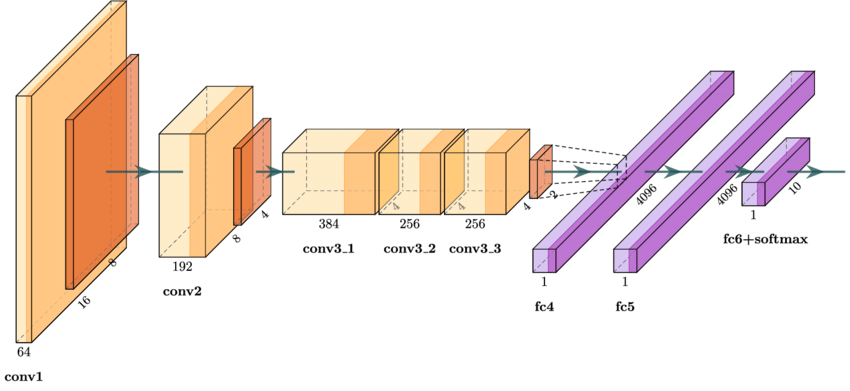
\includegraphics[width=\textwidth]{img/appendixA/alexnet.png}
    \caption{AlexNet architecture.}\label{fig:alexnet}
\end{figure}
\lipsum[1]
\begin{align}
     \vec{\nabla} \cdot \vec{E} \quad &=\quad\frac{\rho}{\epsilon_0} &&\text{Gauss's Law} \\      
    \vec{\nabla} \cdot \vec{B} \quad &=\quad 0 &&\text{Gauss's Law for Magnetism}\\
    \vec{\nabla} \times \vec{E} \quad &=\hspace{10pt}-\frac{\partial{\vec{B}}}{\partial{t}} &&\text{Faraday's Law of Induction} \\ 
    \vec{\nabla} \times \vec{B} \quad &=\quad \mu_0\left( \epsilon_0\frac{\partial{\vec{E}}}{\partial{t}}+\vec{J}\right) &&\text{Ampere's Circuital Law}
\end{align}

We can find more information in~\cite{li2018deep}.


	
	\backmatter
	\bookmarksetup{startatroot}
	\printbibliography[heading=bibintoc]
\end{document}
